\documentclass[./report.tex]{subfiles}
\usepackage[utf8]{inputenc} % Підтримка UTF-8
\usepackage[ukrainian]{babel} % Підтримка української мови
\usepackage[ukrainian=nohyphenation]{hyphsubst} 
\usepackage{booktabs}
\usepackage[T2A]{fontenc} % Кодова таблиця для кирилиці
\usepackage{amsmath, amsfonts} % Для математики, якщо потрібно
\usepackage[a4paper, left=3cm, right=1.5cm, top=2cm, bottom=2cm]{geometry}
\usepackage{fancyhdr}        % Пакет для налаштування колонтитулів
\usepackage{hyperref}        % Для створення посилань
\usepackage{listings}          % Пакет для вставки коду
\usepackage{graphicx}
\usepackage{csvsimple}
\usepackage{parskip}
\usepackage{csquotes}
\usepackage{pgfplotstable}
\usepackage{xcolor}      % For custom colors

\pagestyle{fancy}            % Встановлюємо fancy стиль для колонтитулів
\fancyhf{}                   % Очищуємо всі колонтитули
% Встановлюємо посилання на зміст у лівий верхній кут
\fancyhead[L]{\hyperlink{mytarget}{Зміст}}  % Посилання на зміст
% Встановлюємо нумерацію сторінок у правий верхній кут
\fancyhead[R]{\thepage}
% Прибираємо колонтитули з першої сторінки
\thispagestyle{plain}
% Прибираємо колонтитули для першої сторінки
\fancypagestyle{plain}{
    \fancyhf{}  % Очищуємо колонтитули
    \renewcommand{\headrulewidth}{0pt}  % Вимикаємо лінію колонтитулів
}
\hypersetup{
    colorlinks=true,        % Enable colored links
    linkcolor=red!50!black,      % Color for internal links
    citecolor=red!50!black,      % Color for citations
    filecolor=red!50!black,      % Color for file links
    urlcolor=red!50!black        % Color for external URLs
}

\graphicspath{{../../../}}

\setlength{\emergencystretch}{3cm}

\usepackage{subfiles}

\begin{document}

\section{EDA}

\begin{enumerate}
  \item Чи впливає швидкість вітру (windspeed) на концентрацію частинок PM2.5 і PM10
    
  \quad \textit{Був використаний trimmed набір даних}

  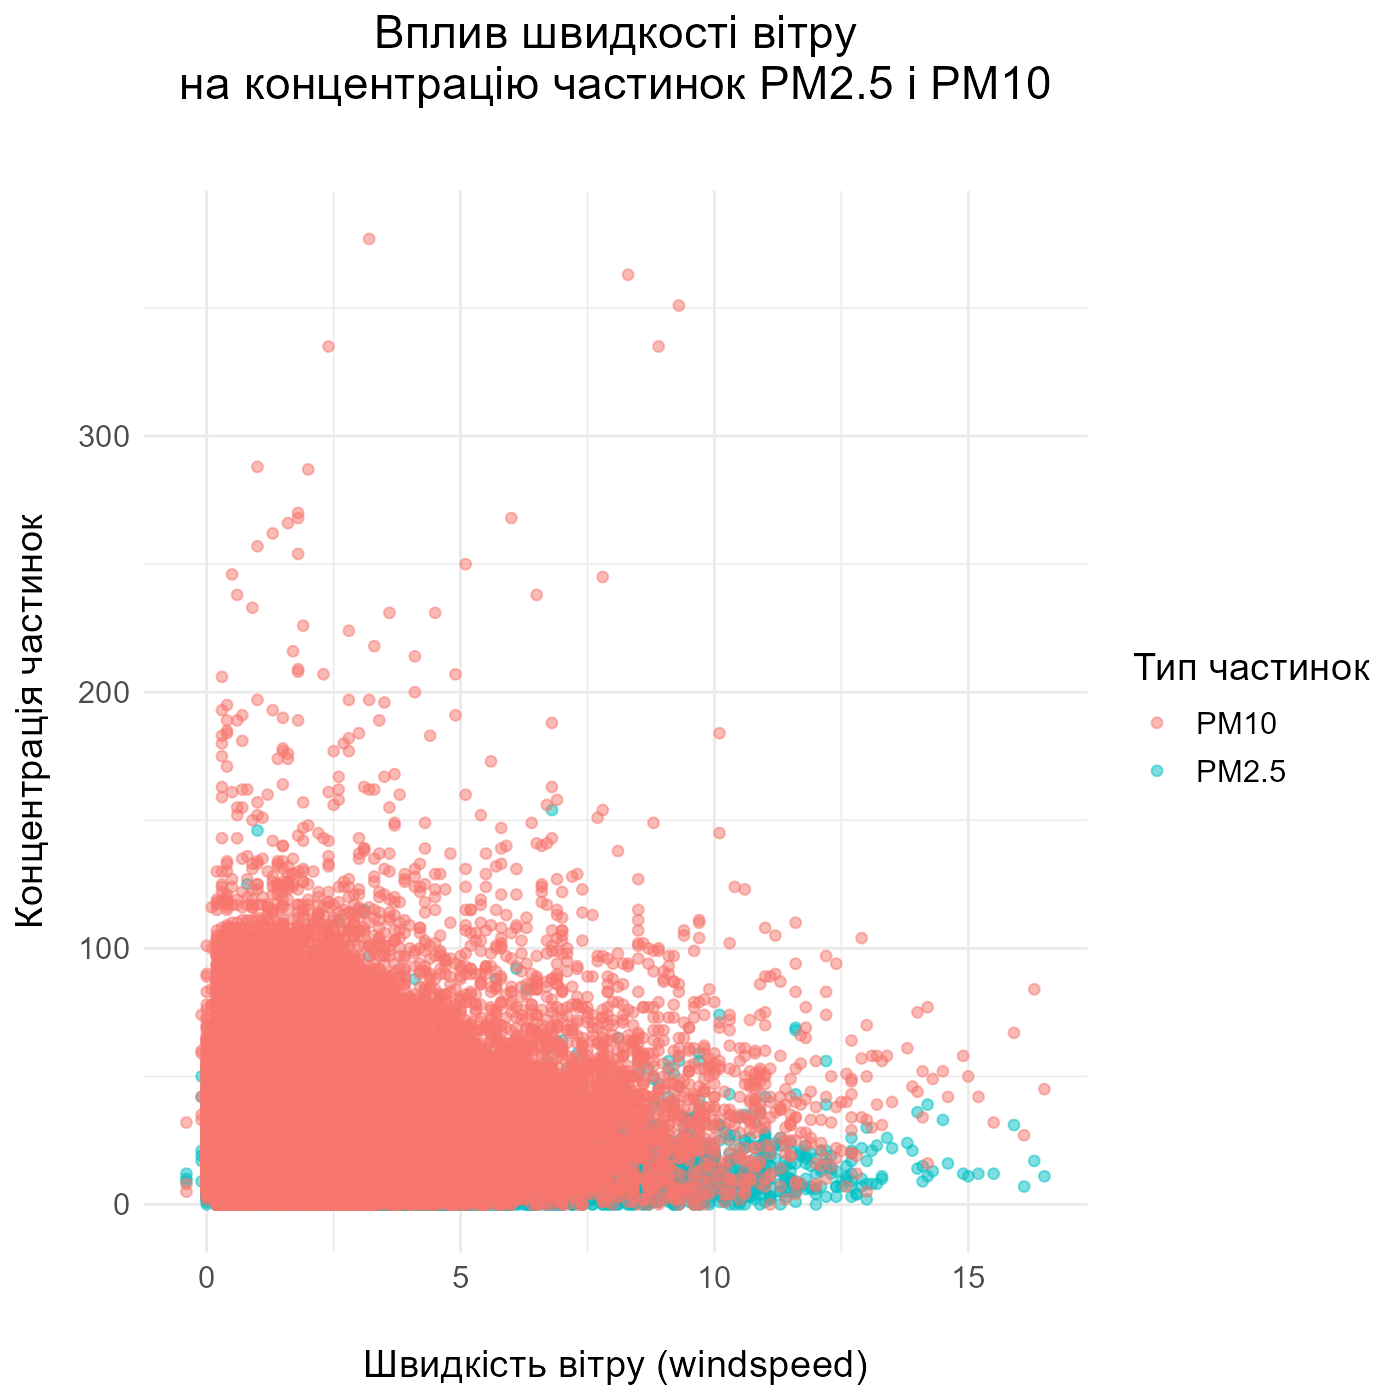
\includegraphics[width=6in]{plots/question1/wind_speed_vs_pm.png}

  Гістограма розподілу для PM.5:
    
  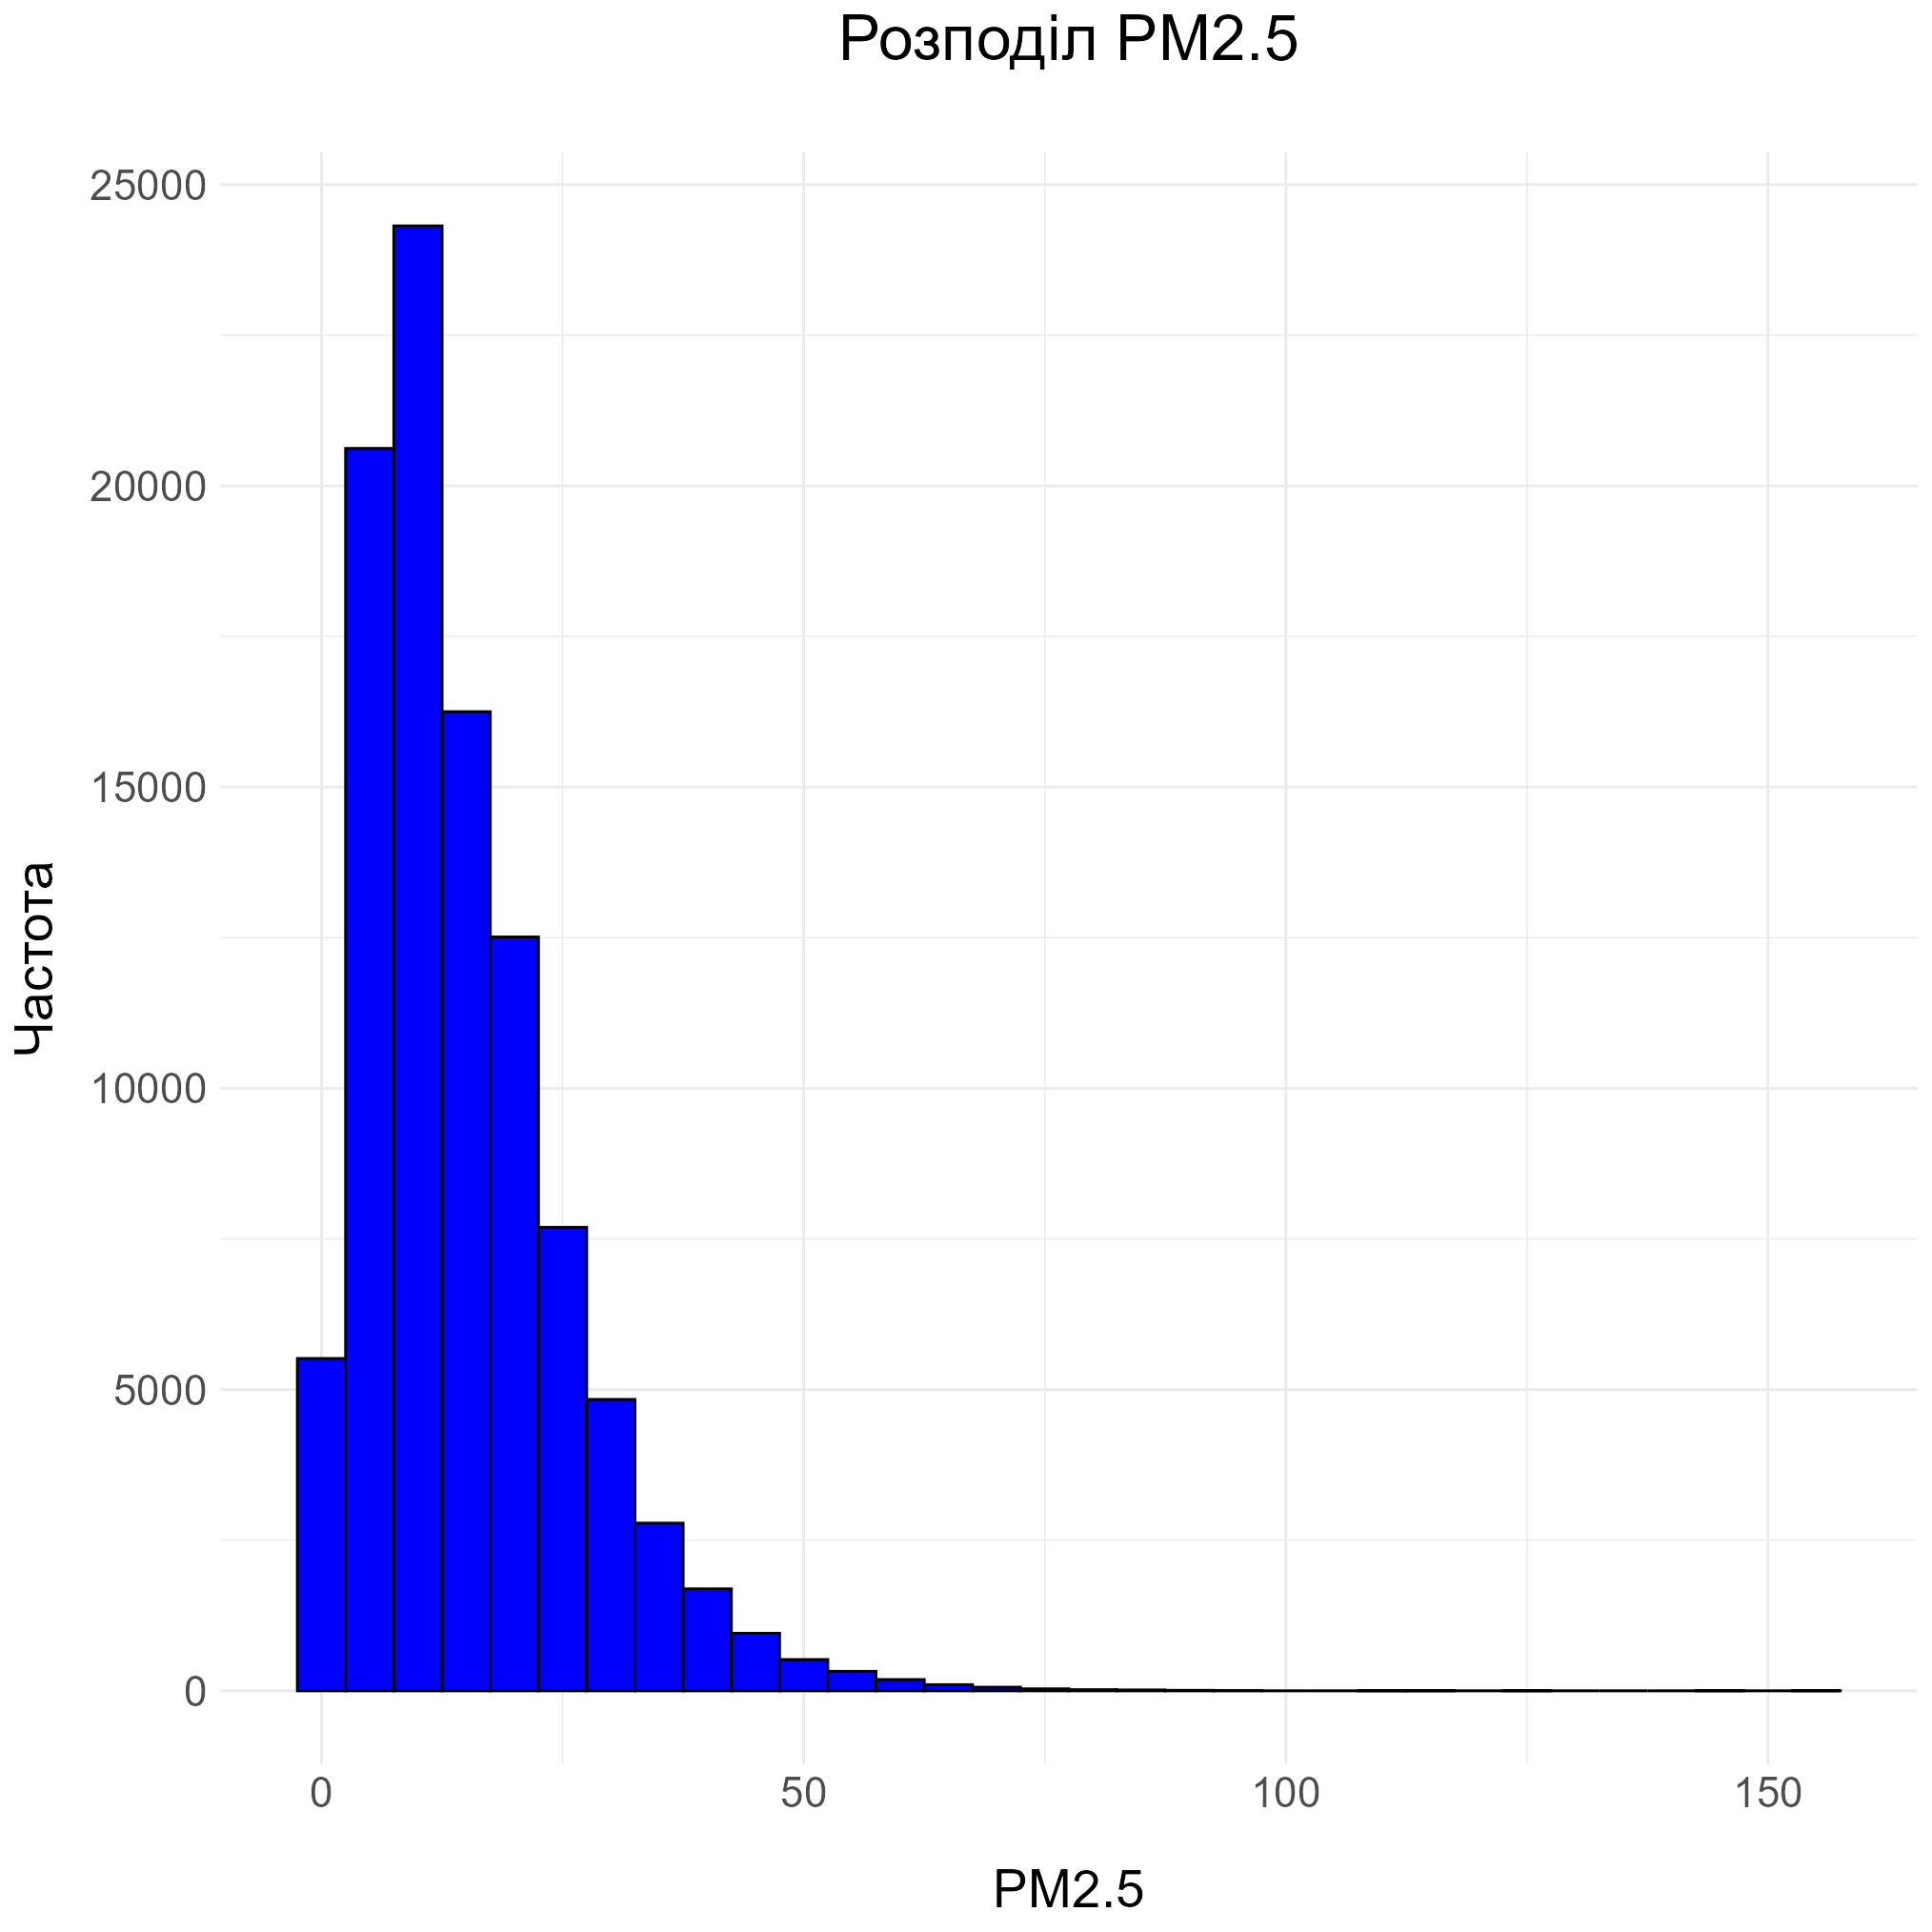
\includegraphics[width=6in]{plots/question1/pm2_5_gist.png}

  Кореляційна матриця:

  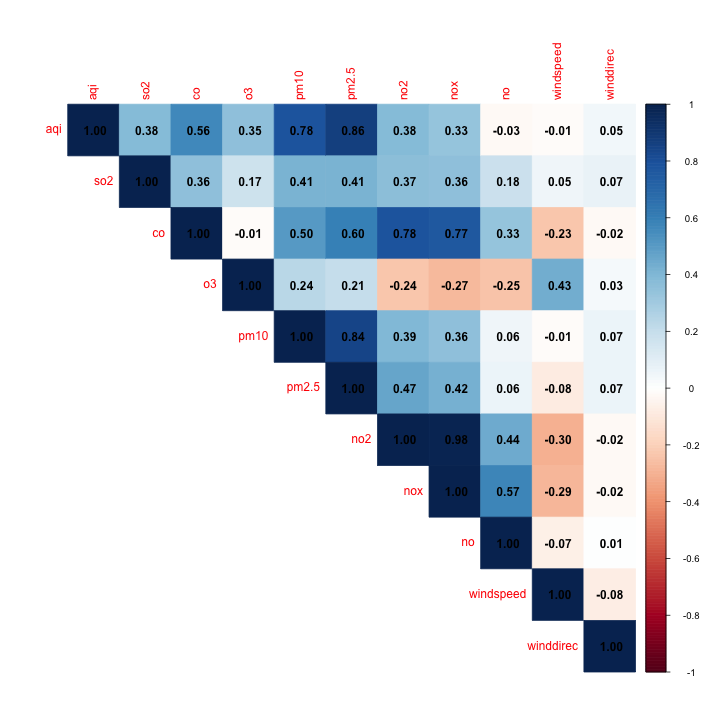
\includegraphics[width=6in]{plots/question1/corr_matrix_plot.png}

  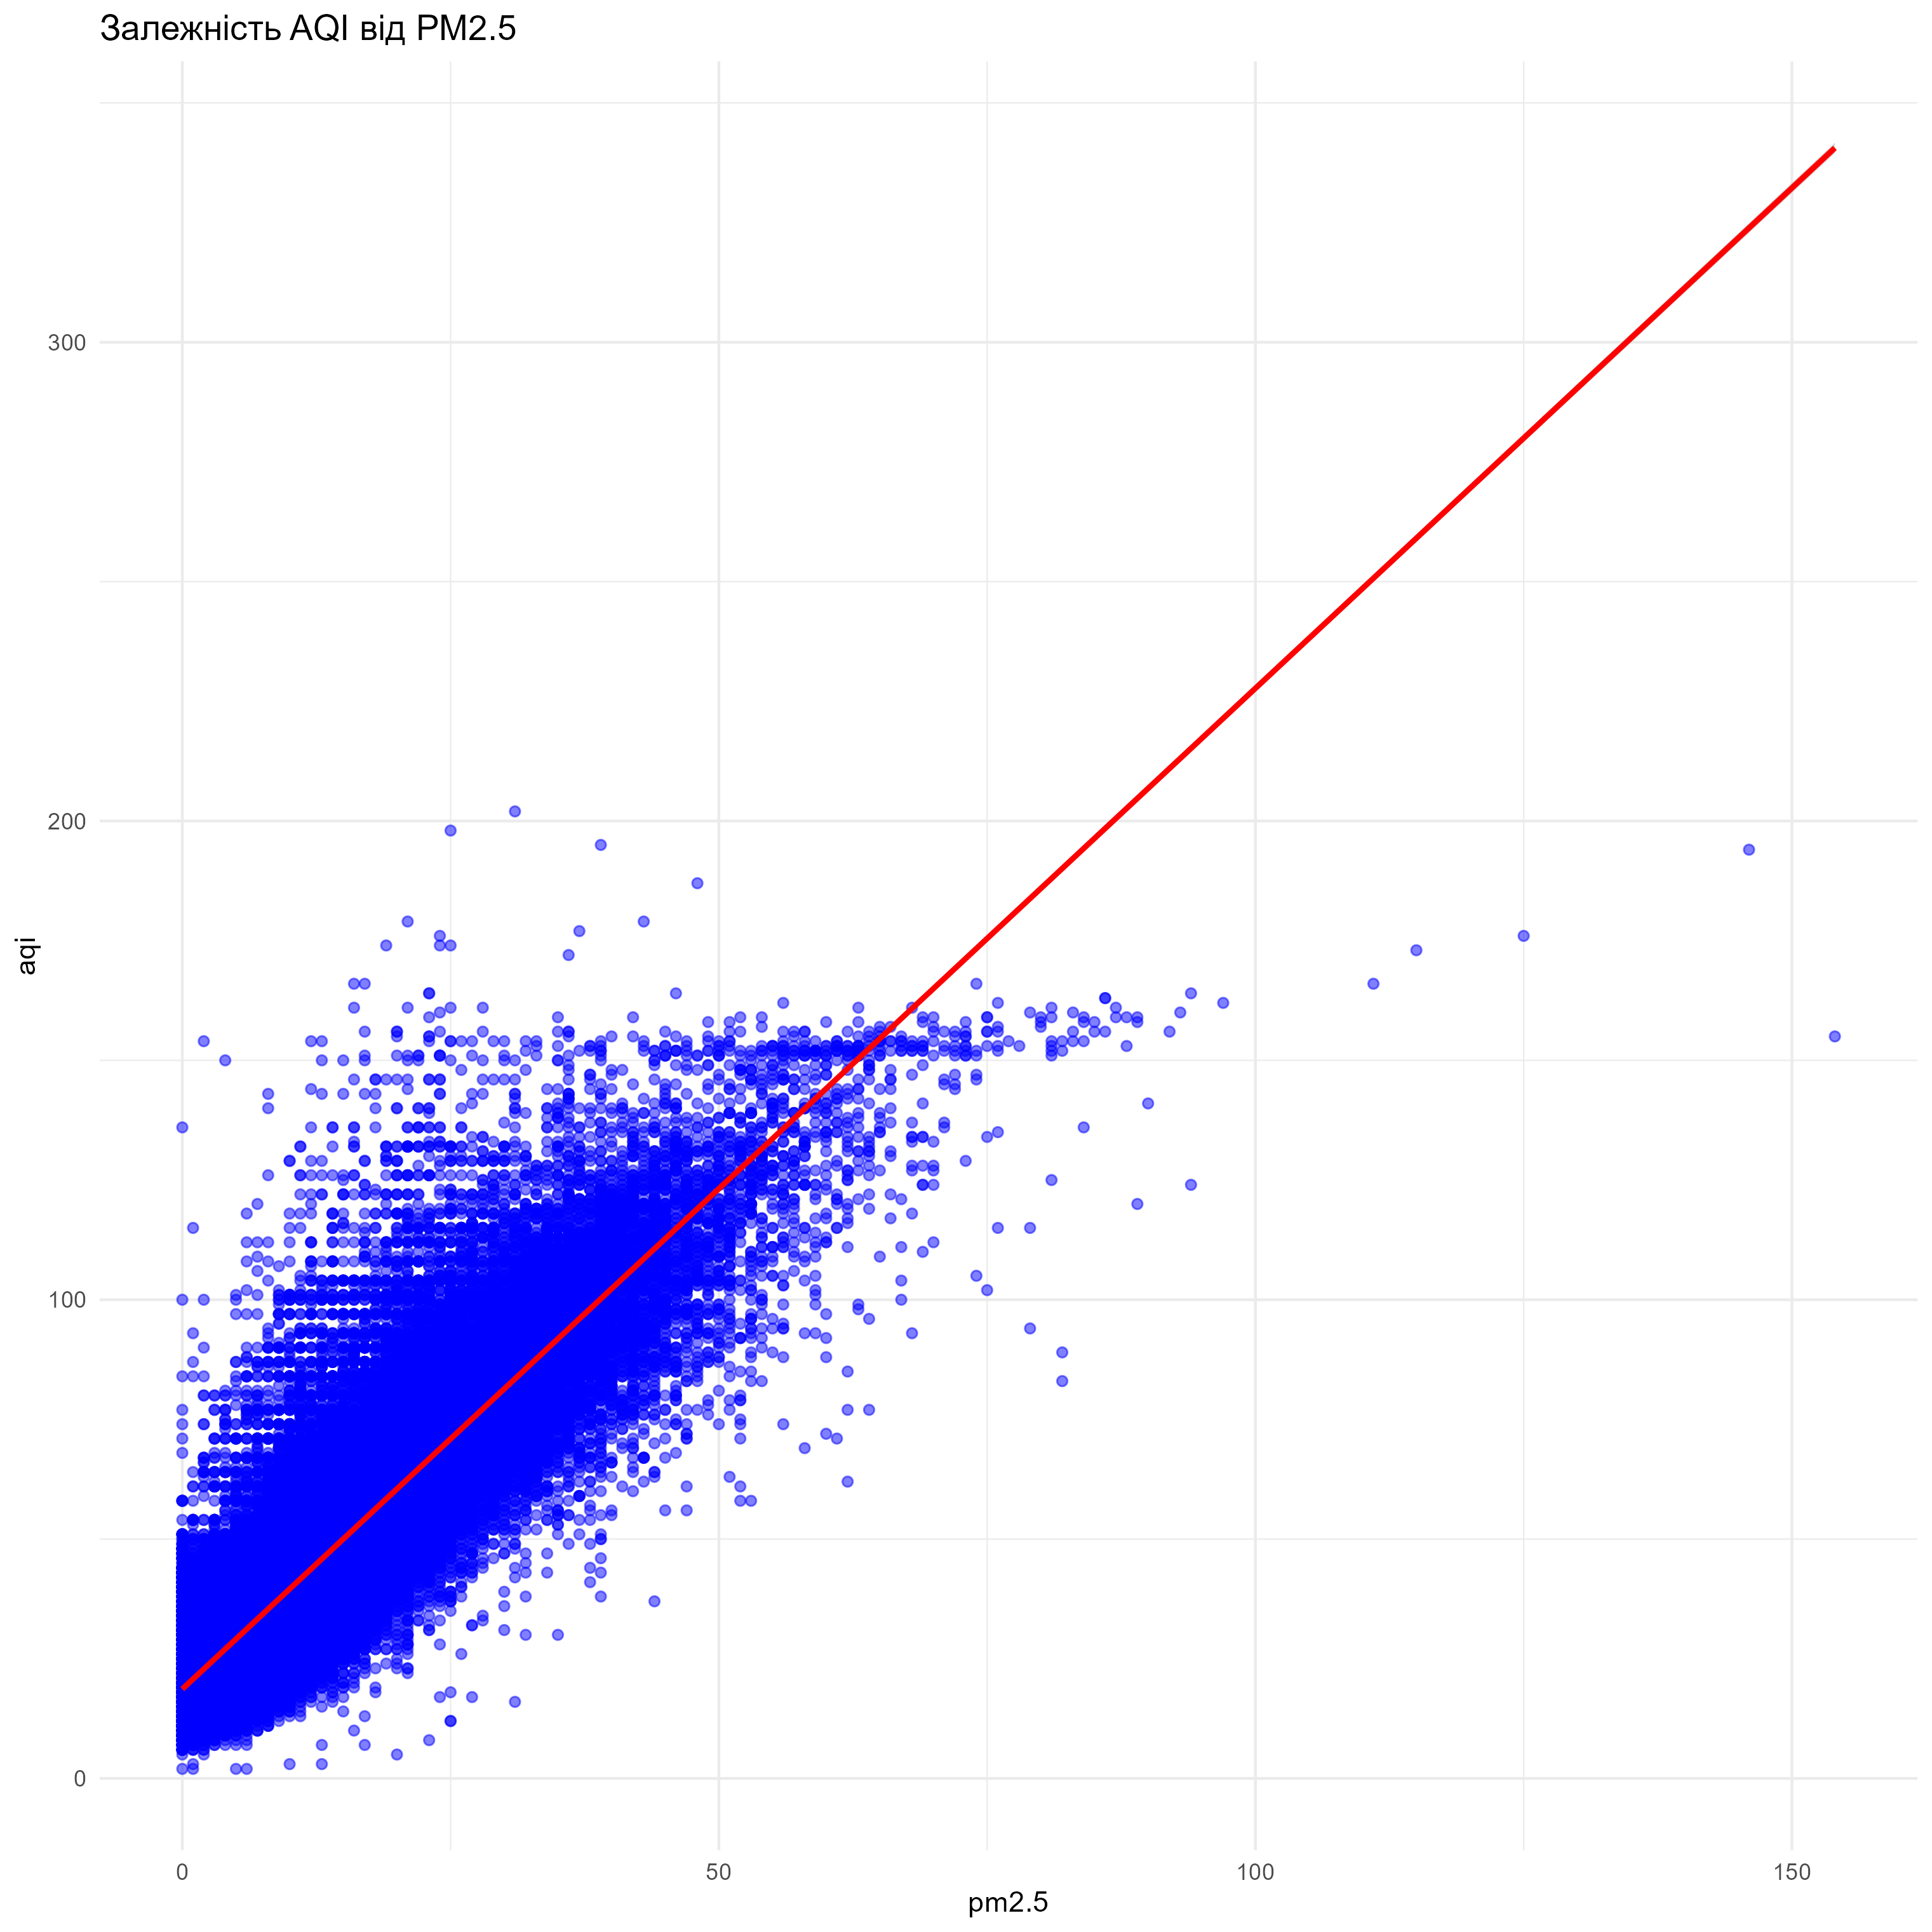
\includegraphics[width=6in]{plots/question1/aqi_pm2_5_diagram.png}

  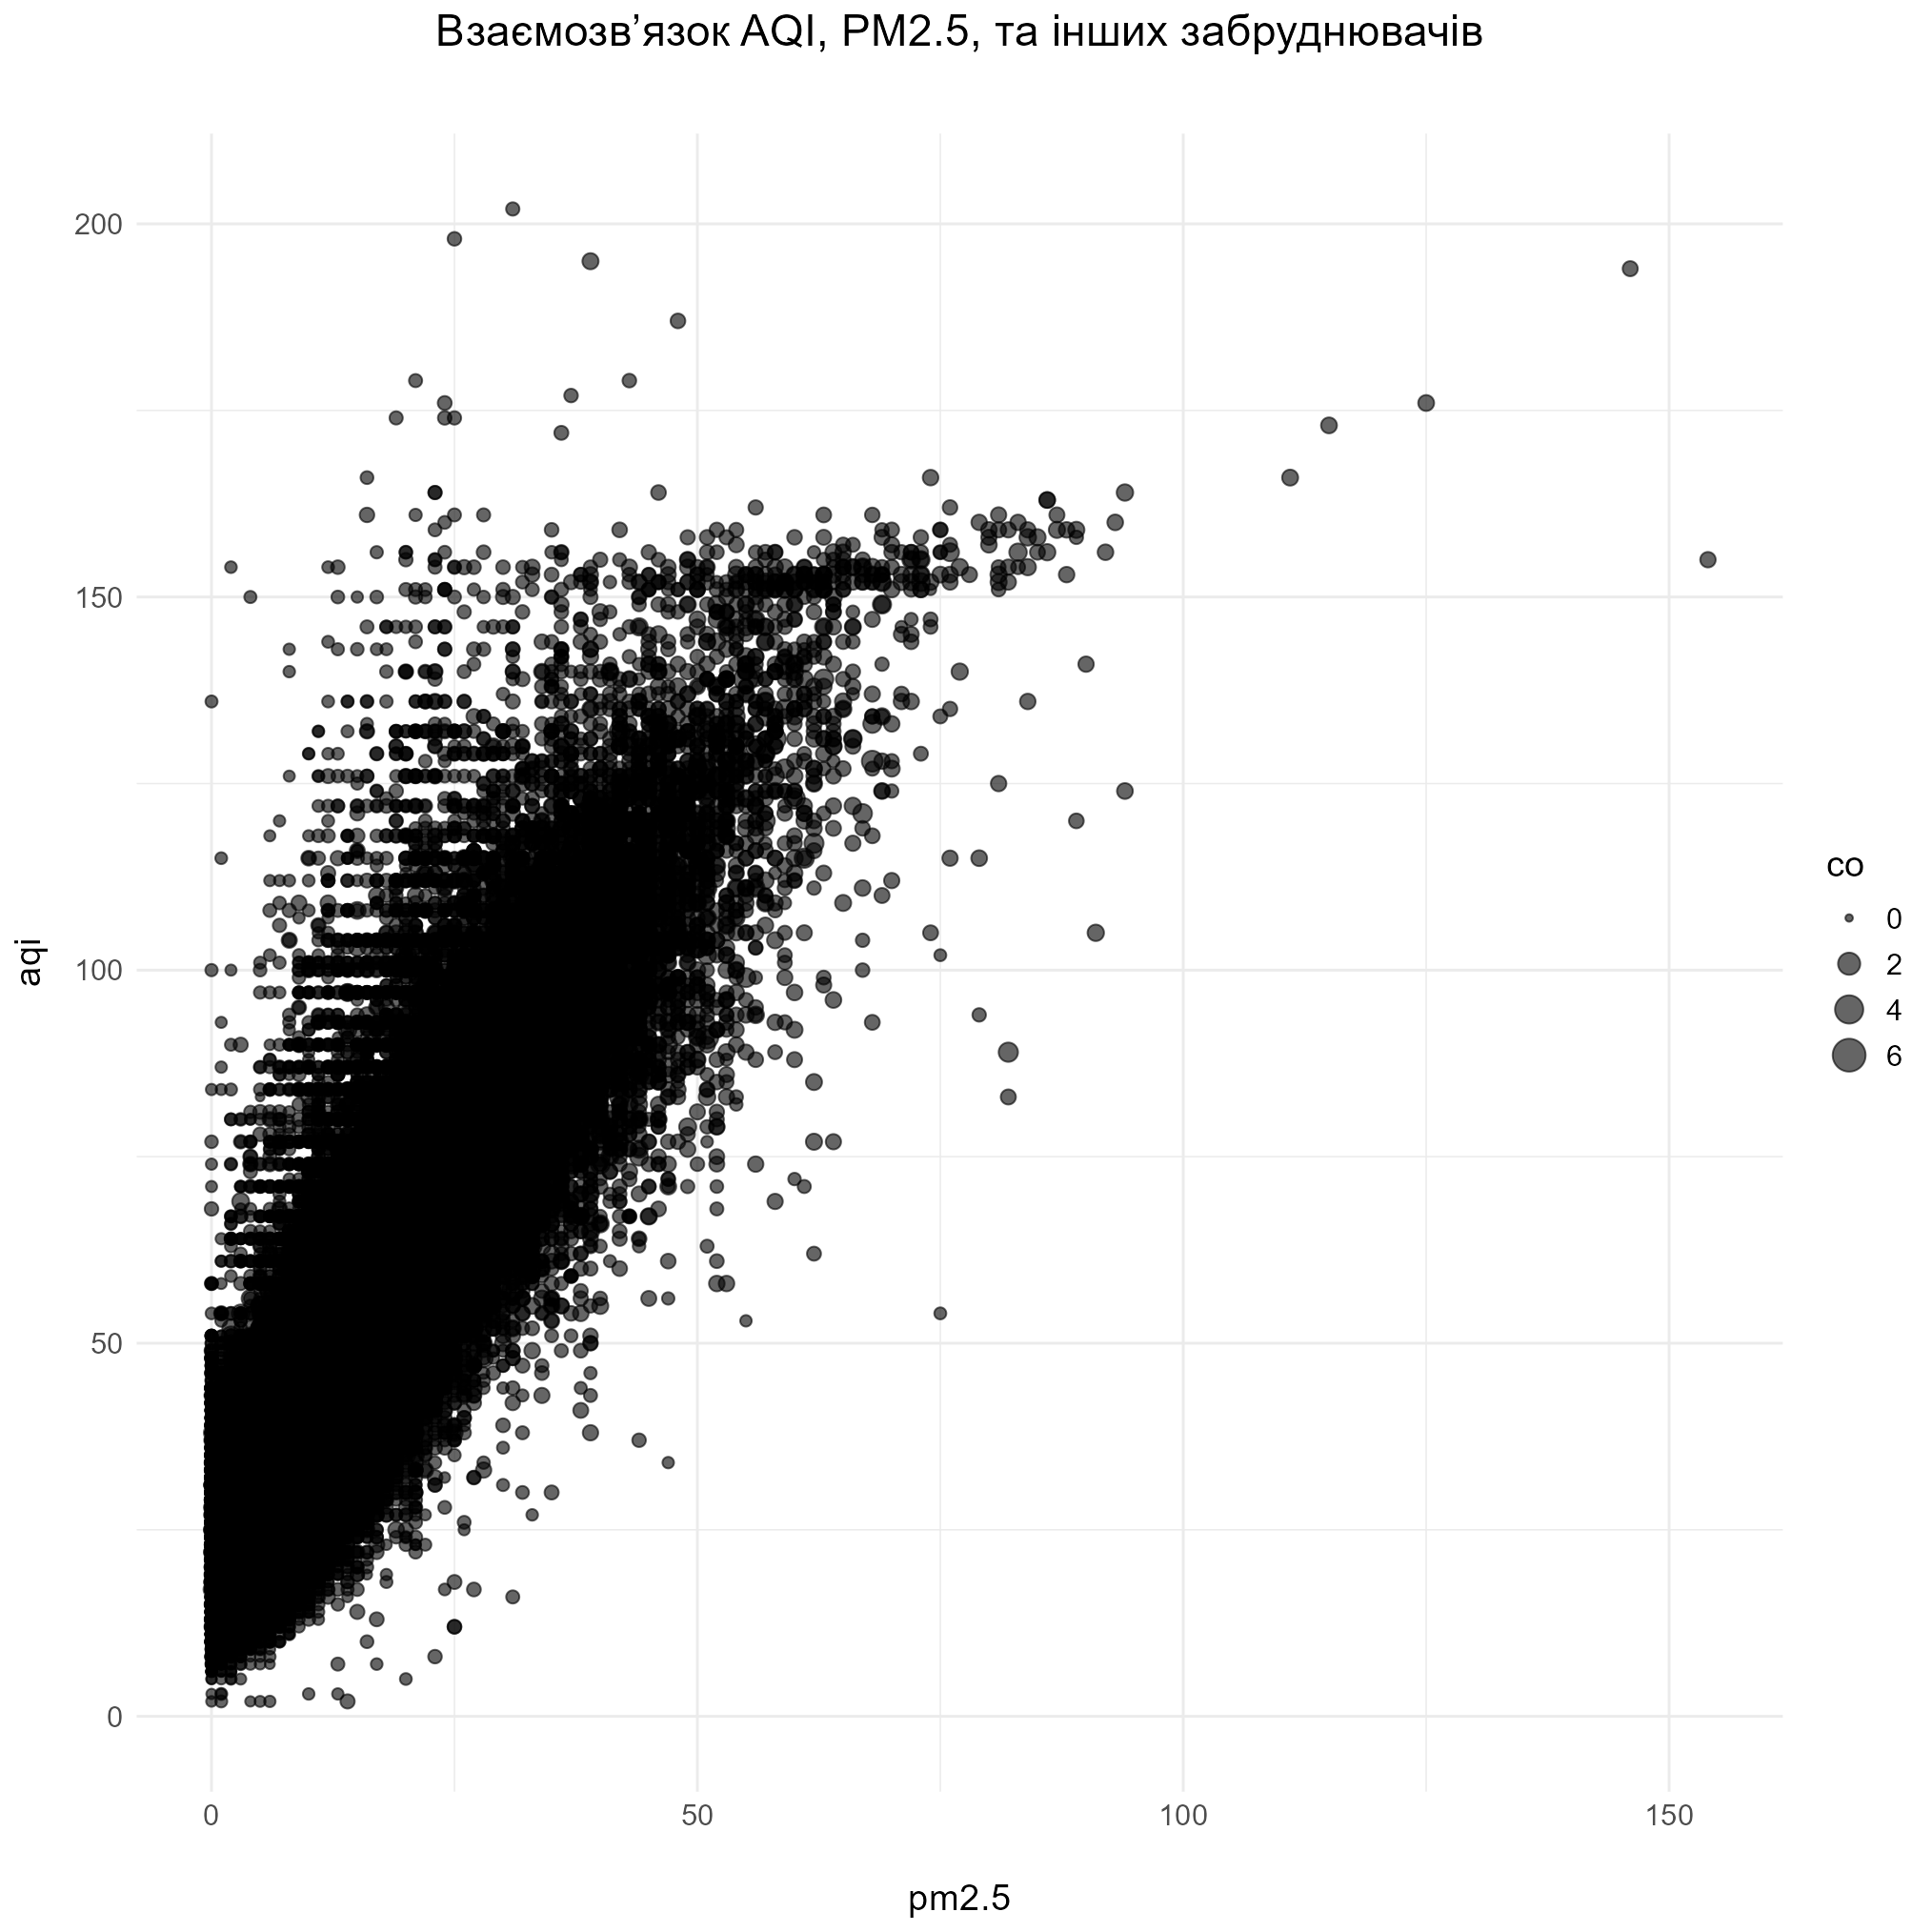
\includegraphics[width=6in]{plots/question1/aqi_pm_polutants.png}

  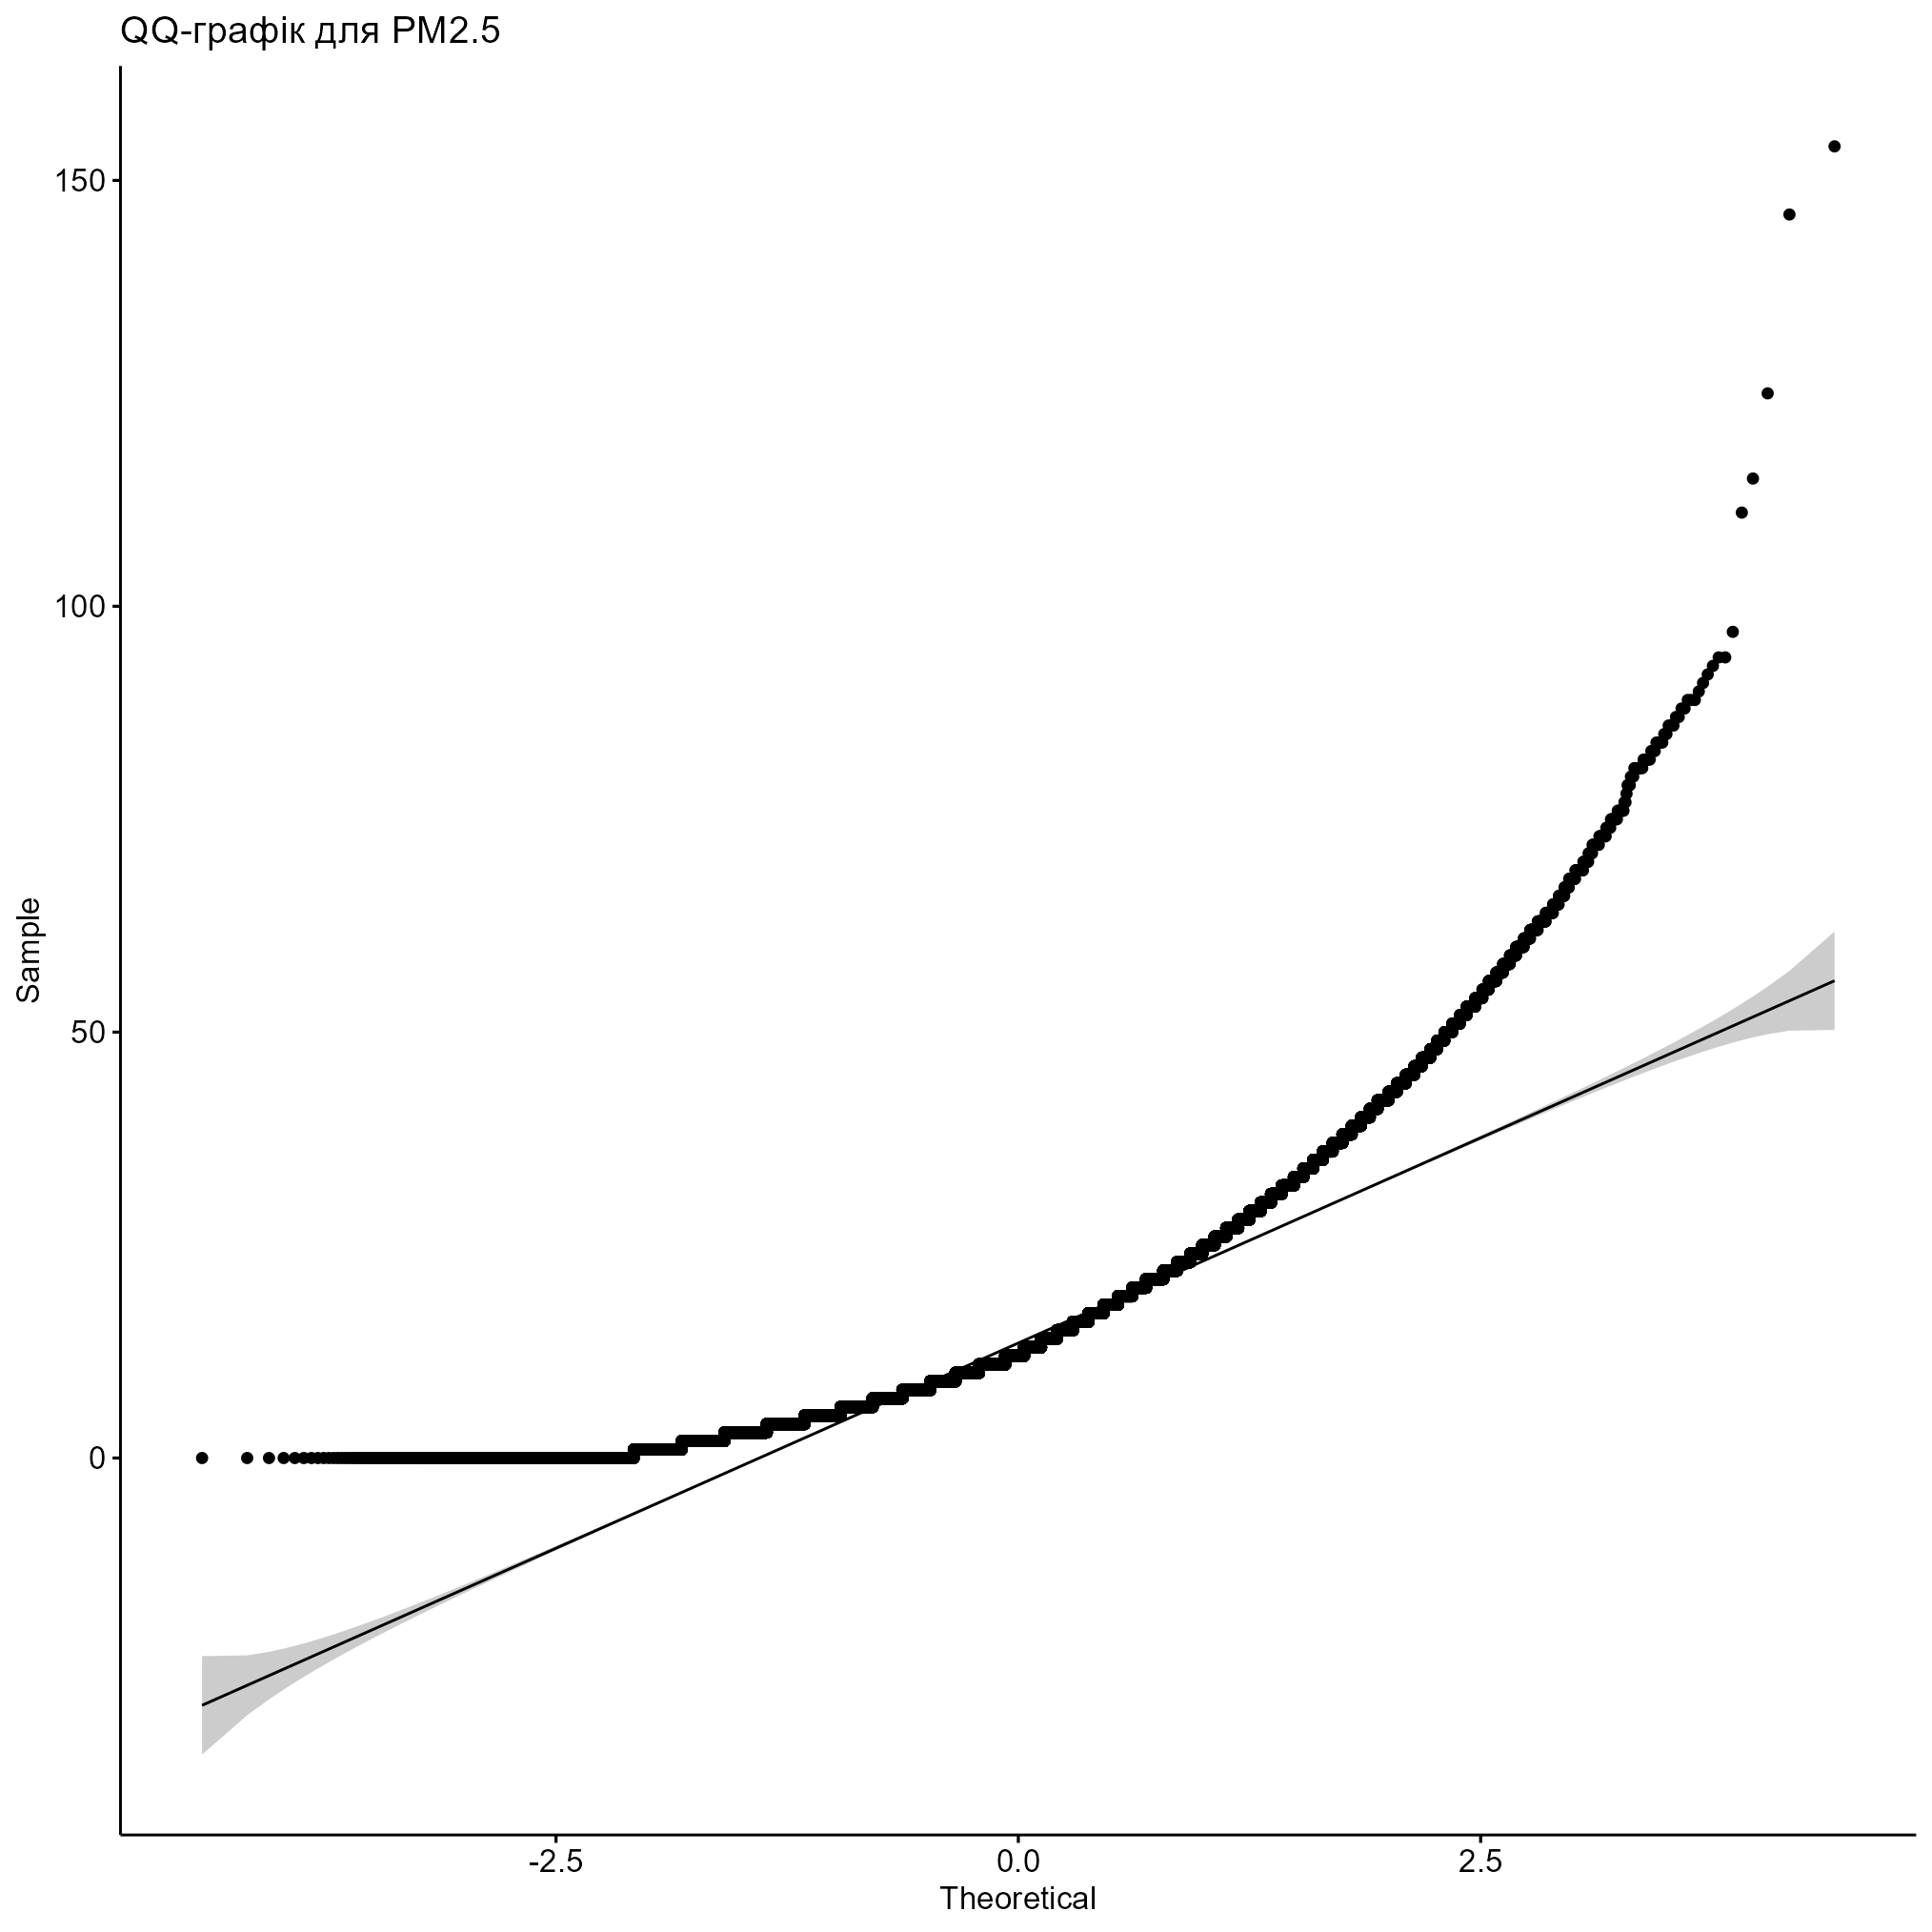
\includegraphics[width=6in]{plots/question1/qq_pm2_5.png}

  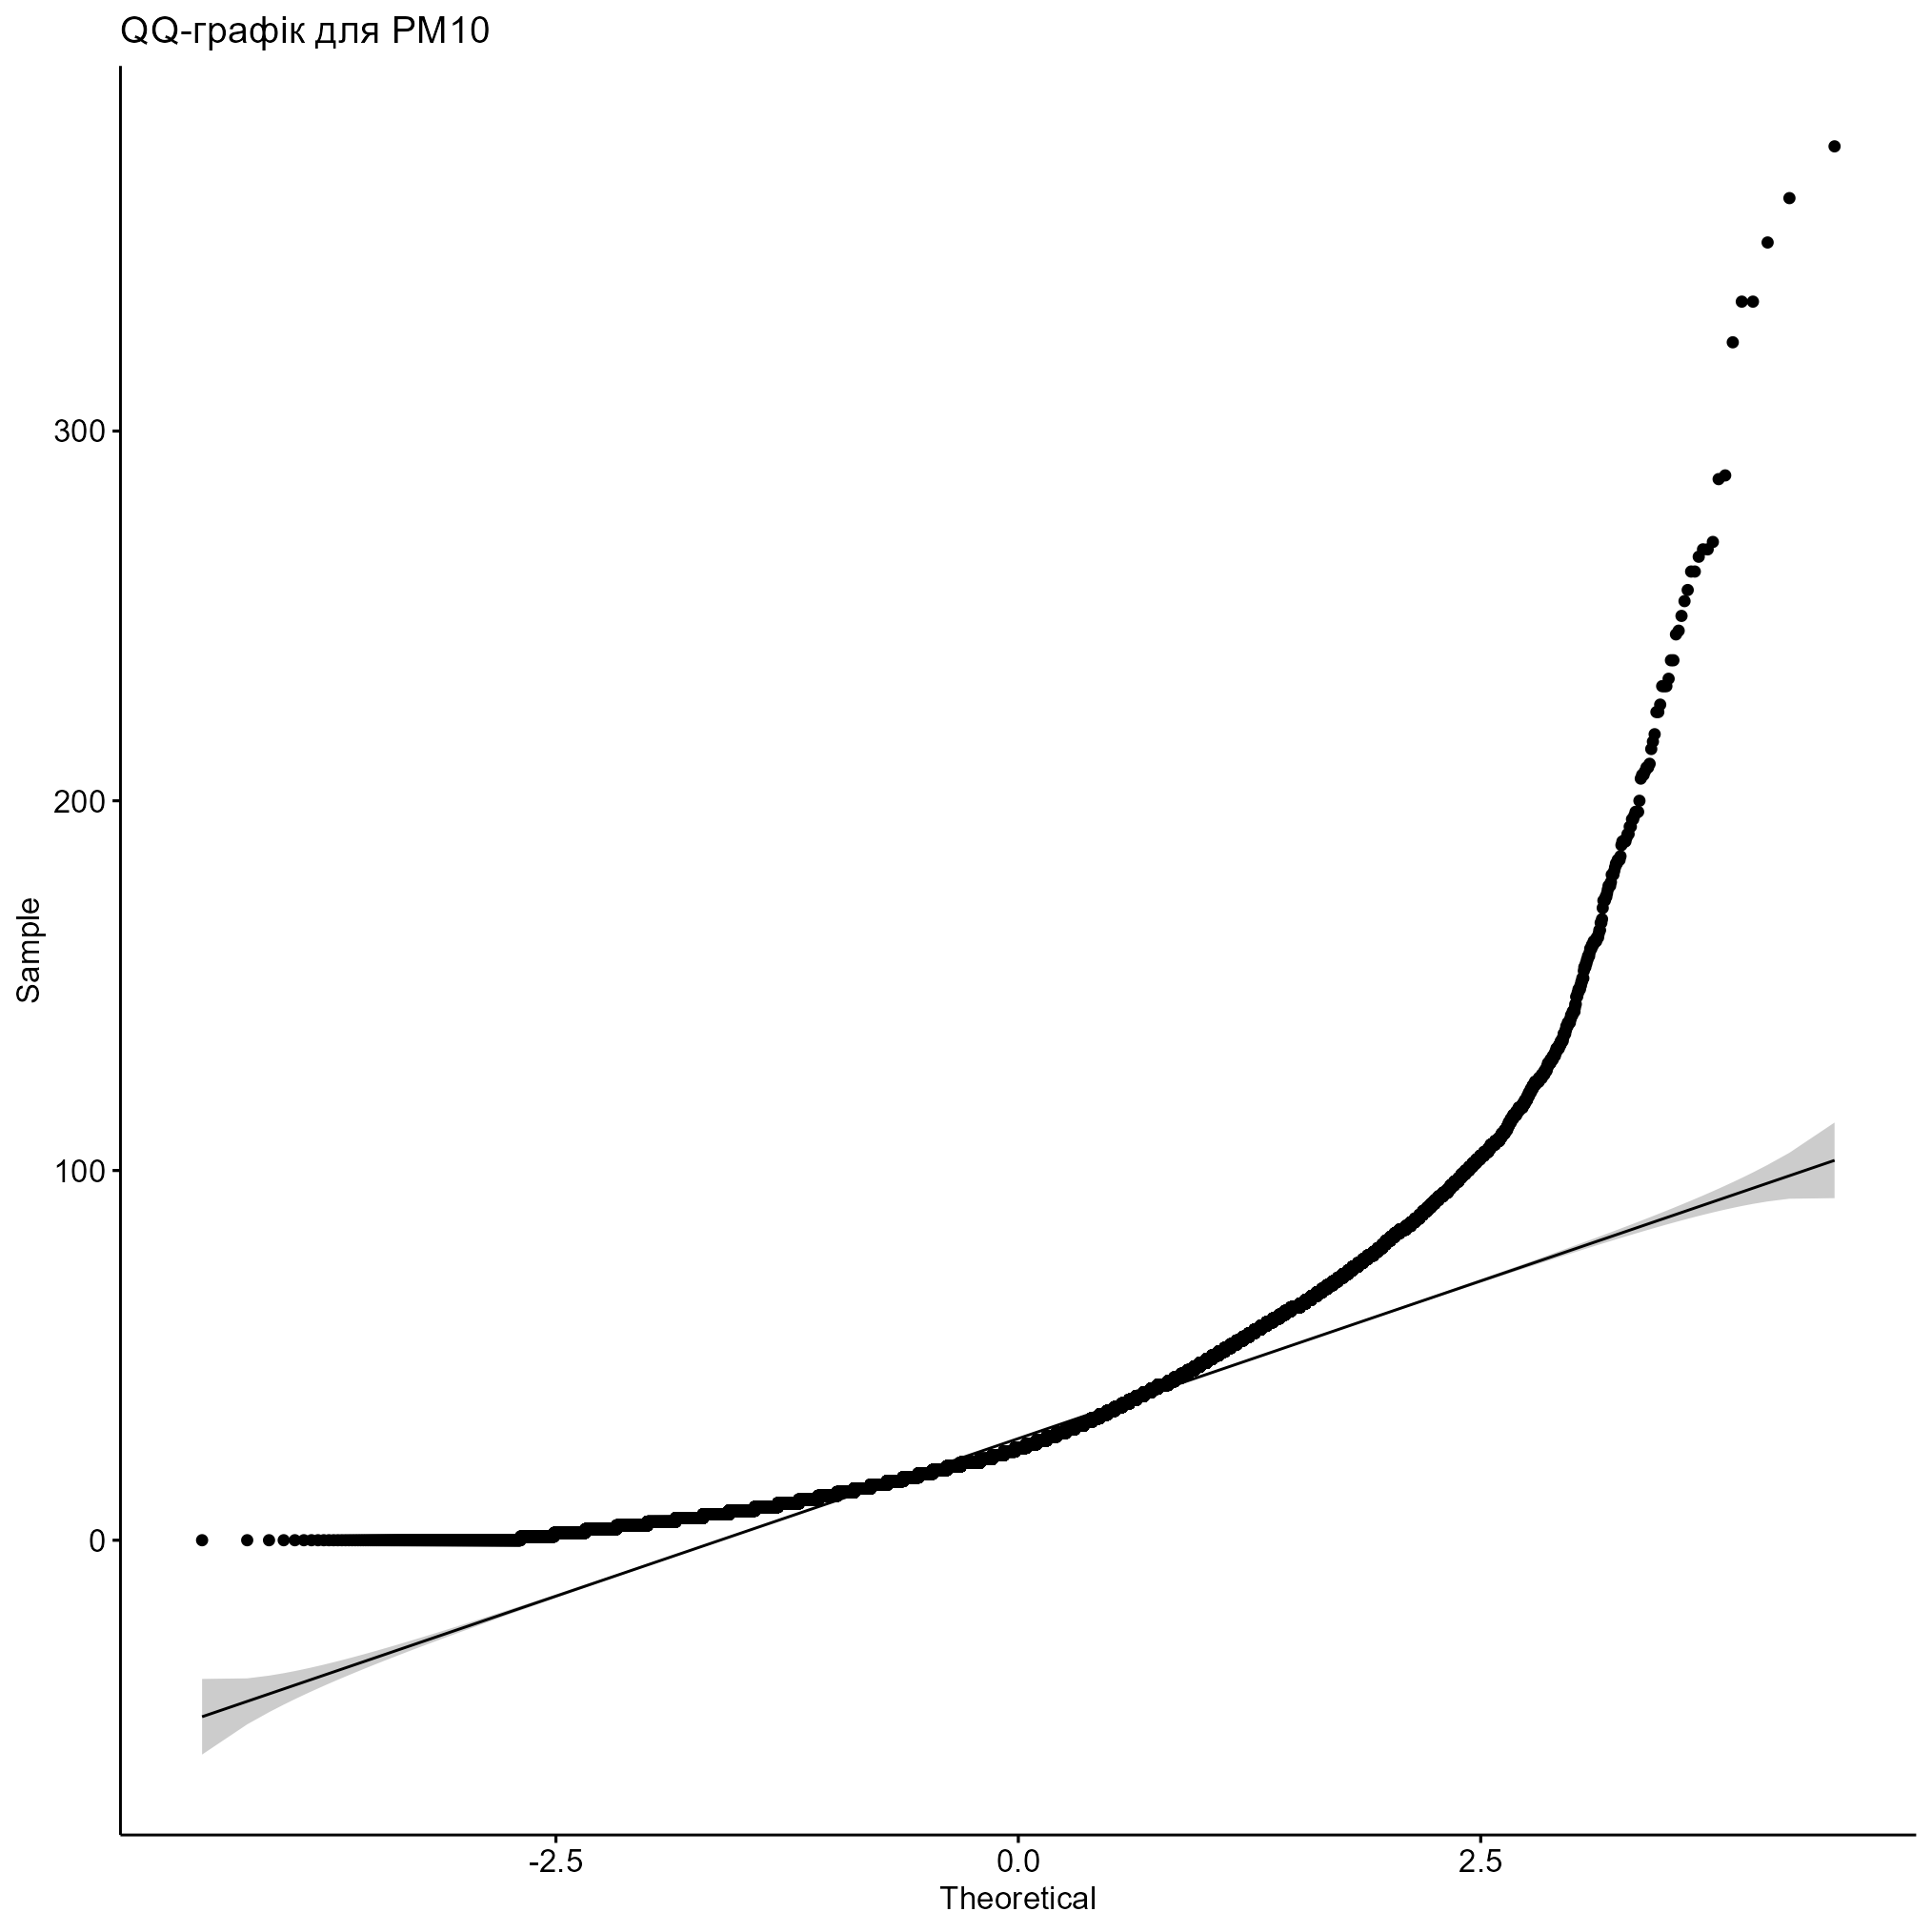
\includegraphics[width=6in]{plots/question1/qq_pm10.png}

  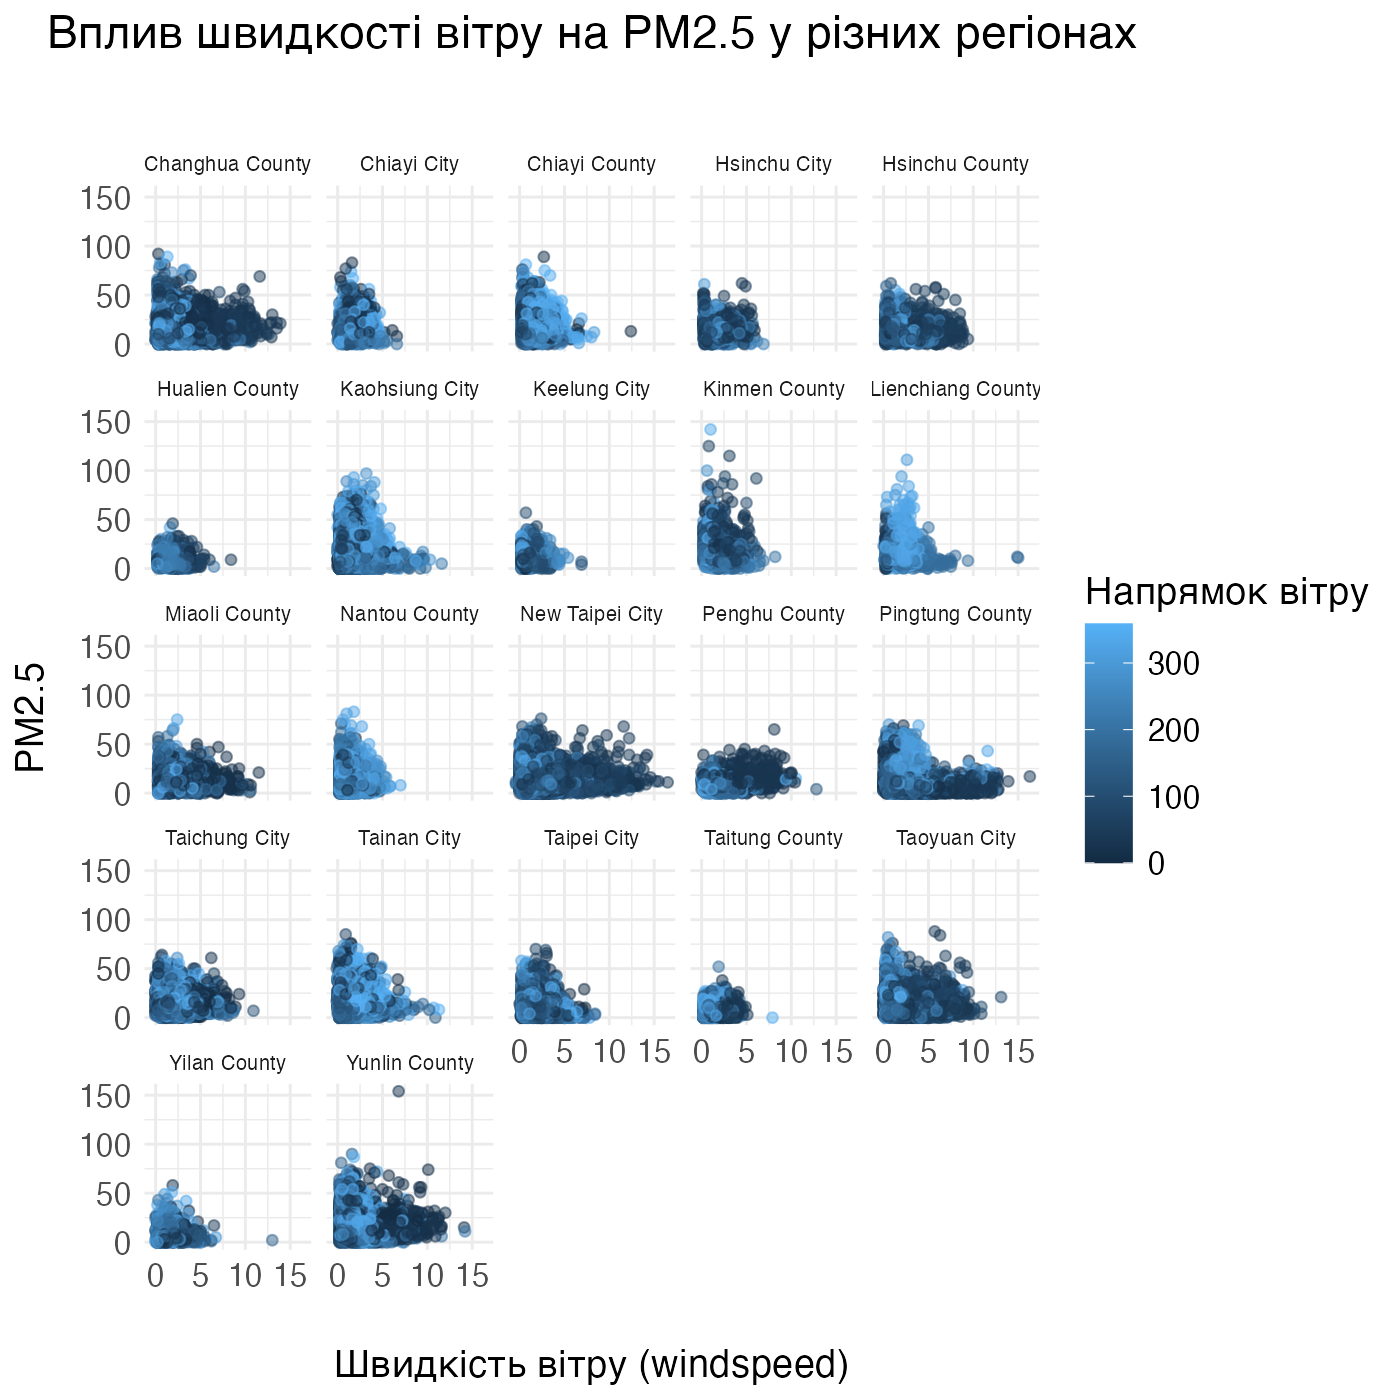
\includegraphics[width = 6in]{plots/question1/scatter_pm2_5_region.png}

  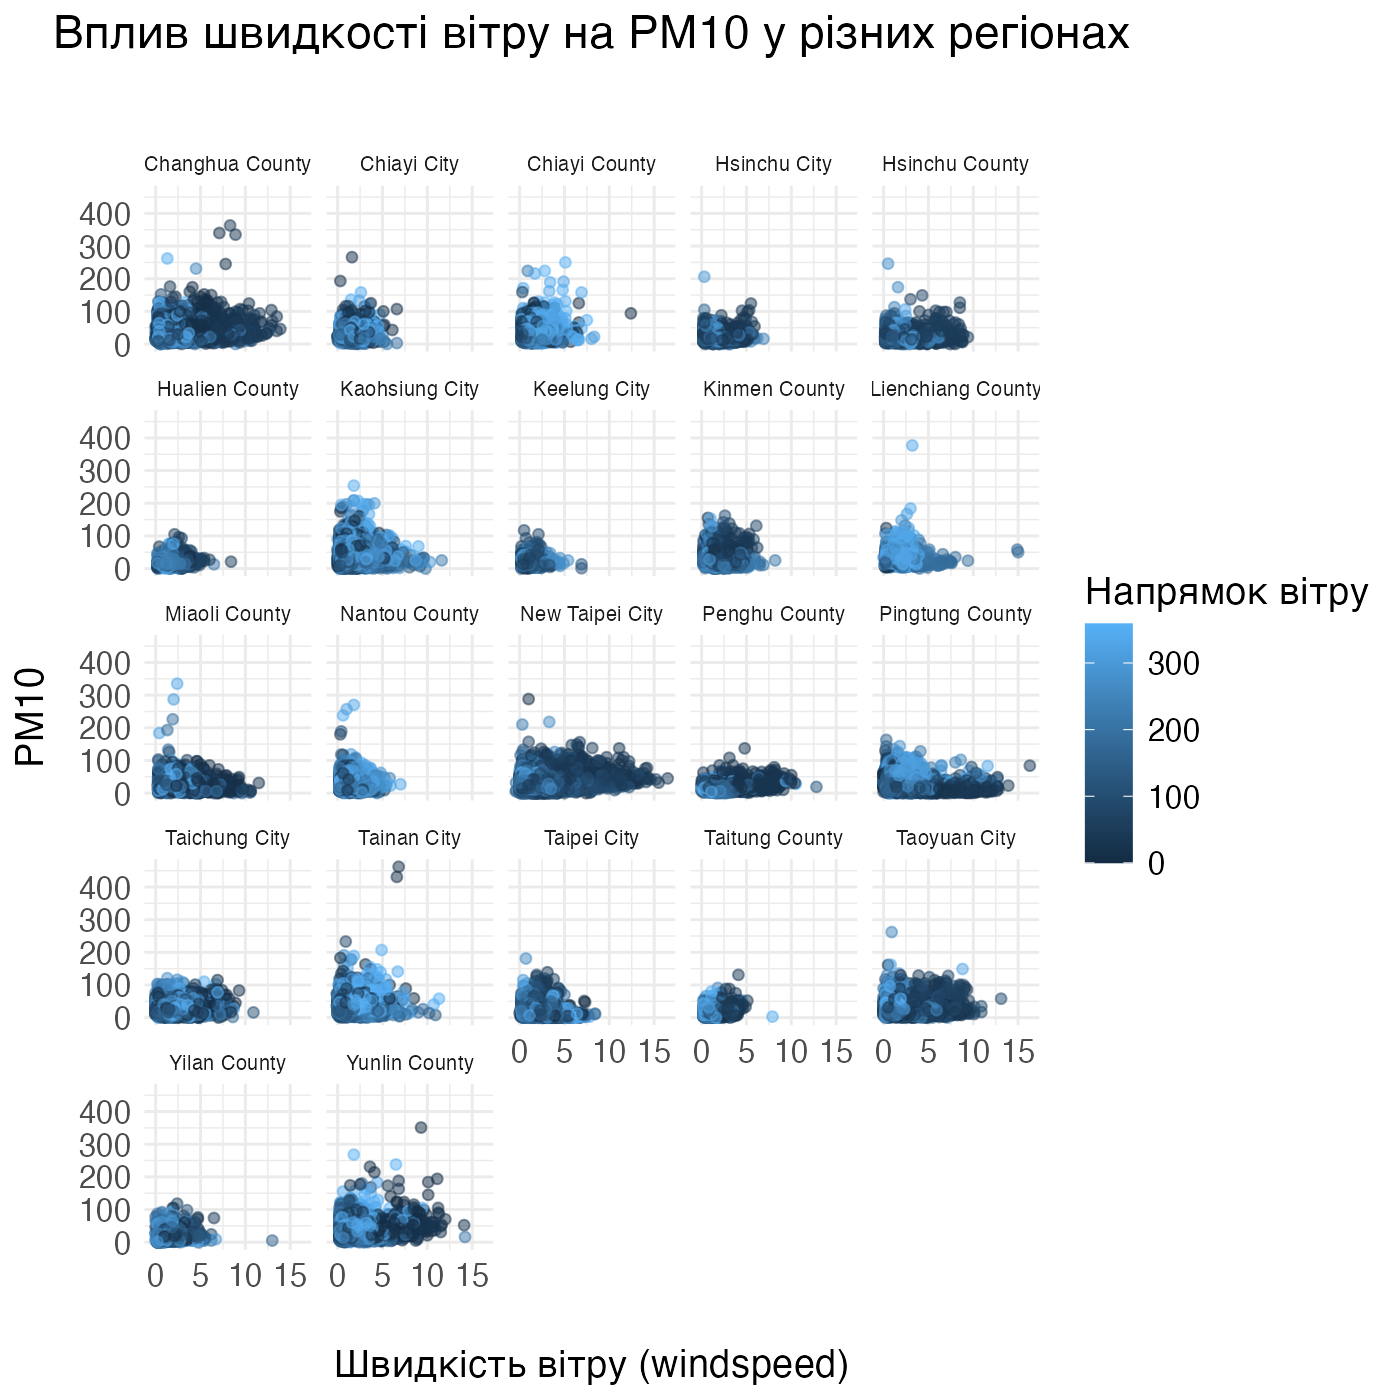
\includegraphics[width = 6in]{plots/question1/scatter_pm10_region.png}
    
  \item Як зміни в концентрації ($O_3$) та $SO_2$ впливають на загальний рівень забруднення повітря (AQI)?
    
  \quad \textit{Був використаний trimmed набір даних}

  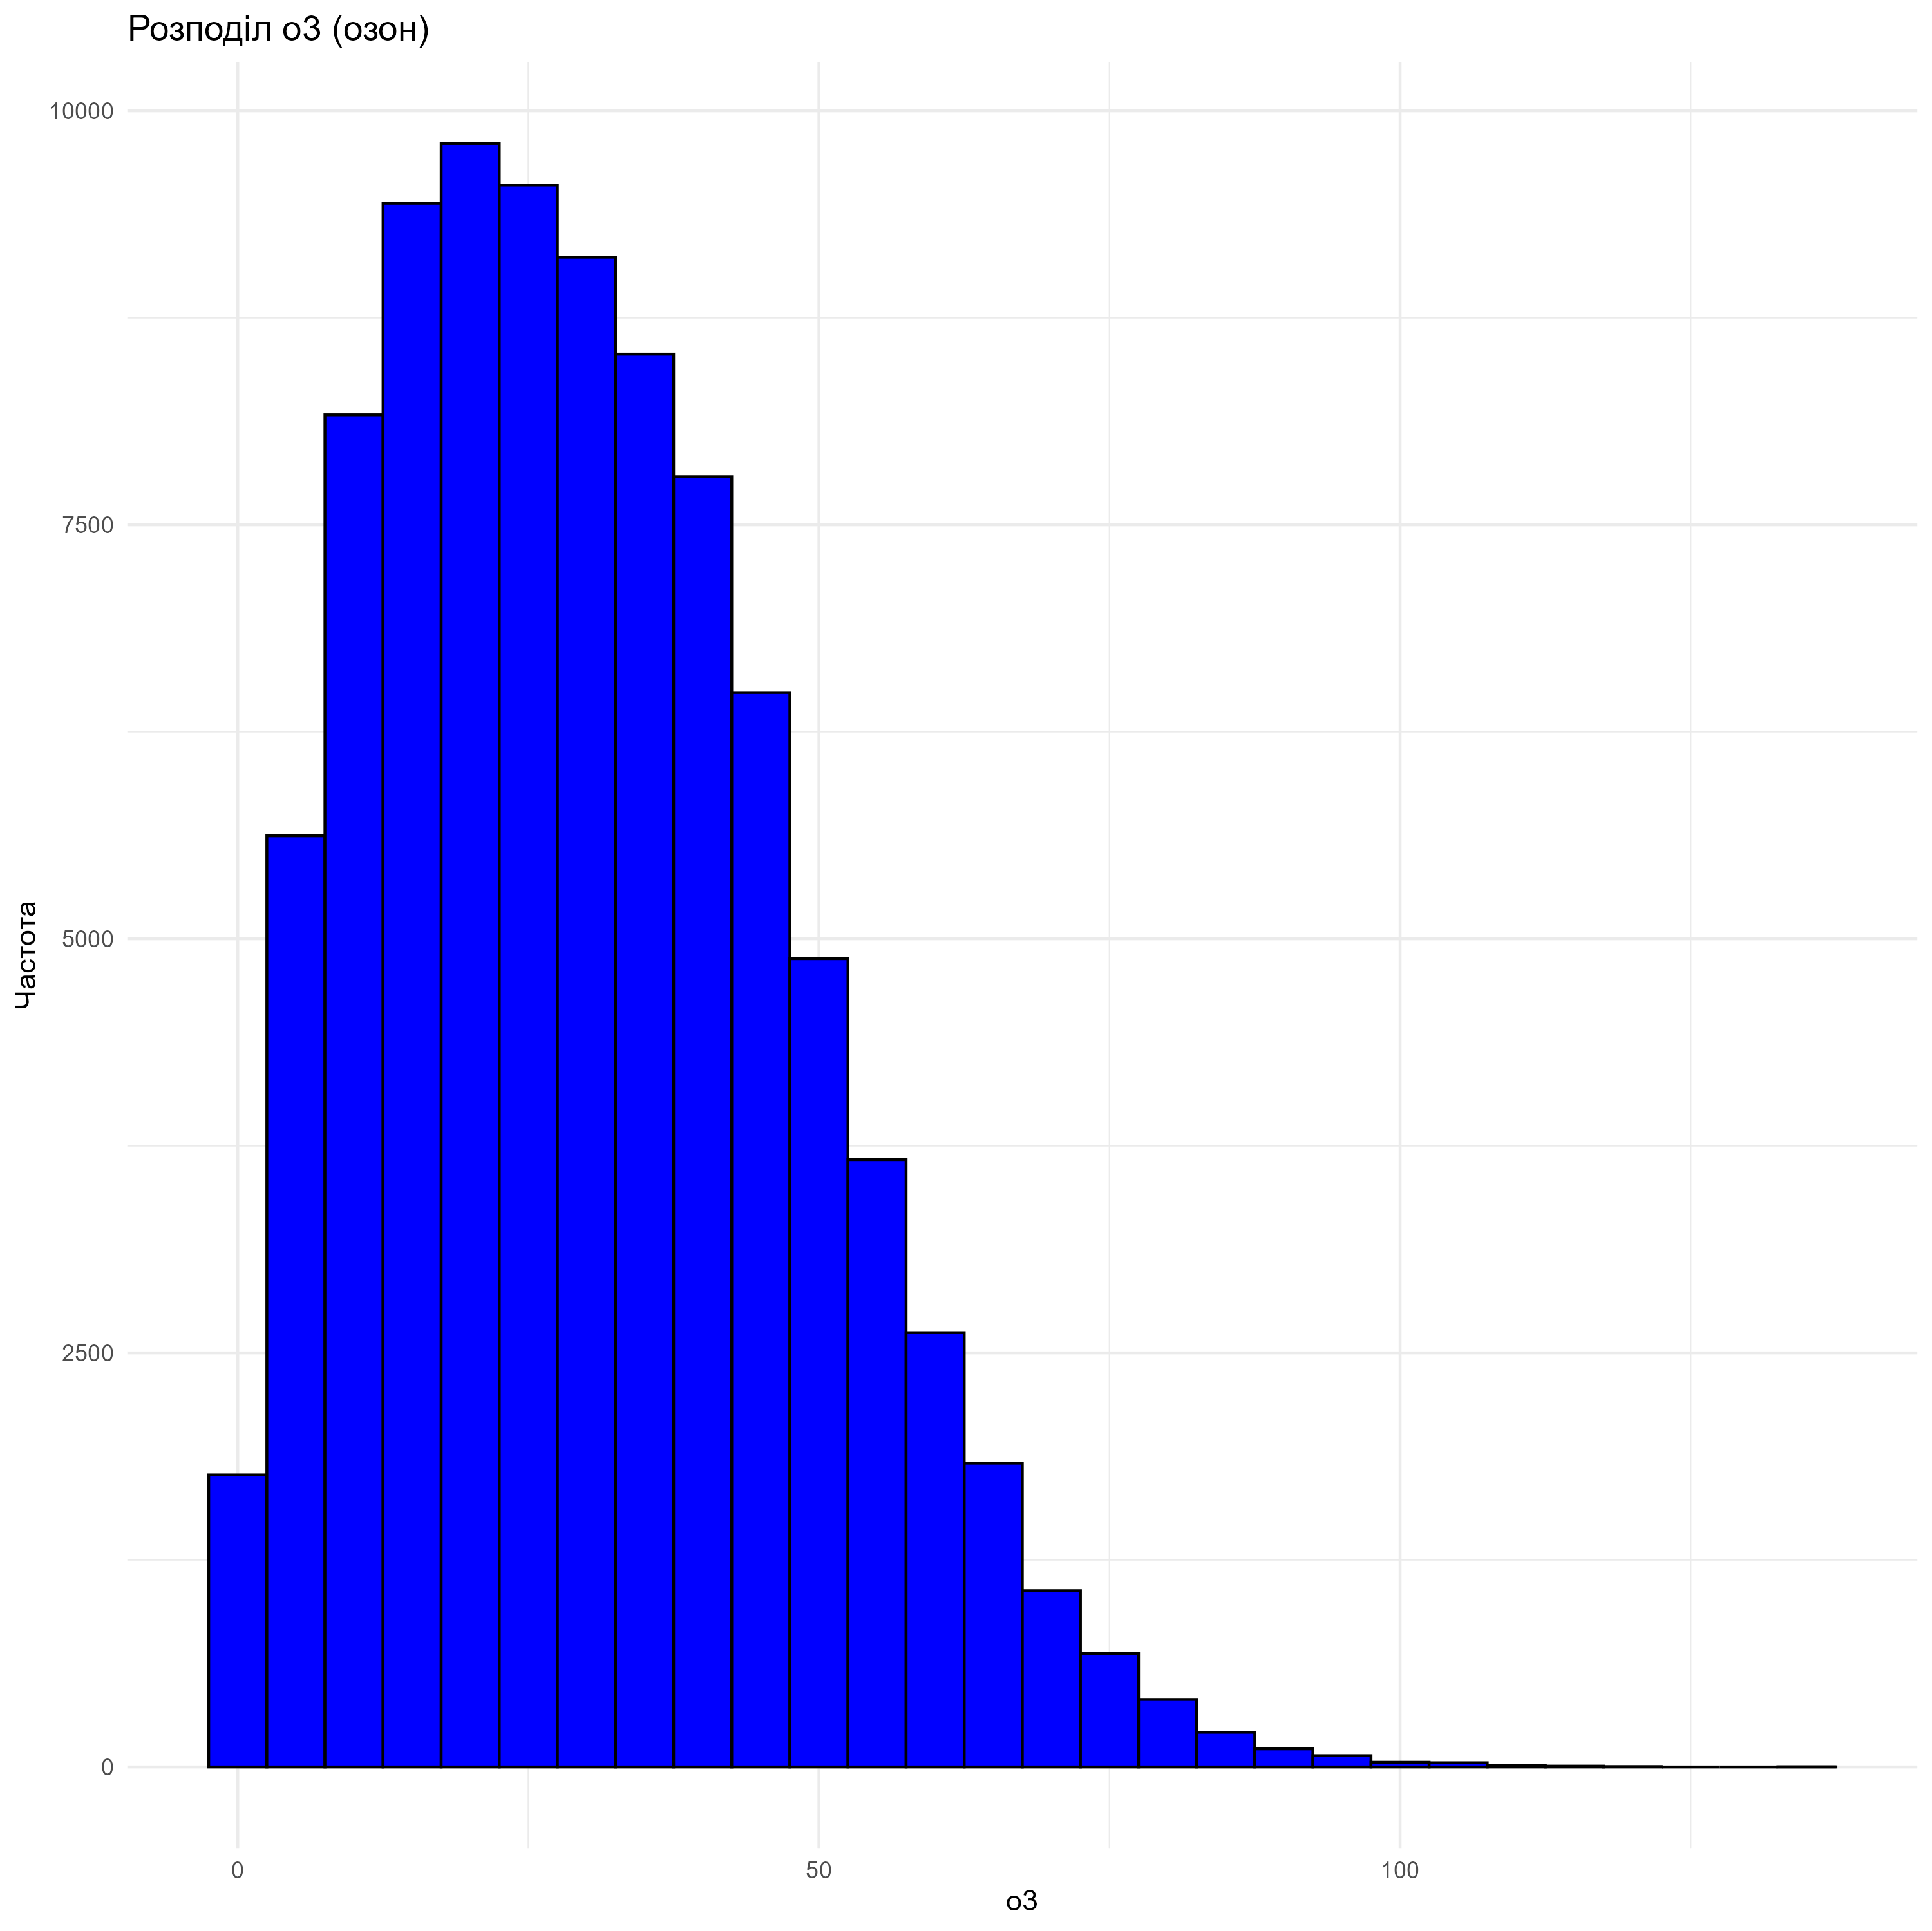
\includegraphics[width=6in]{plots/question2/o3_plot.png}

  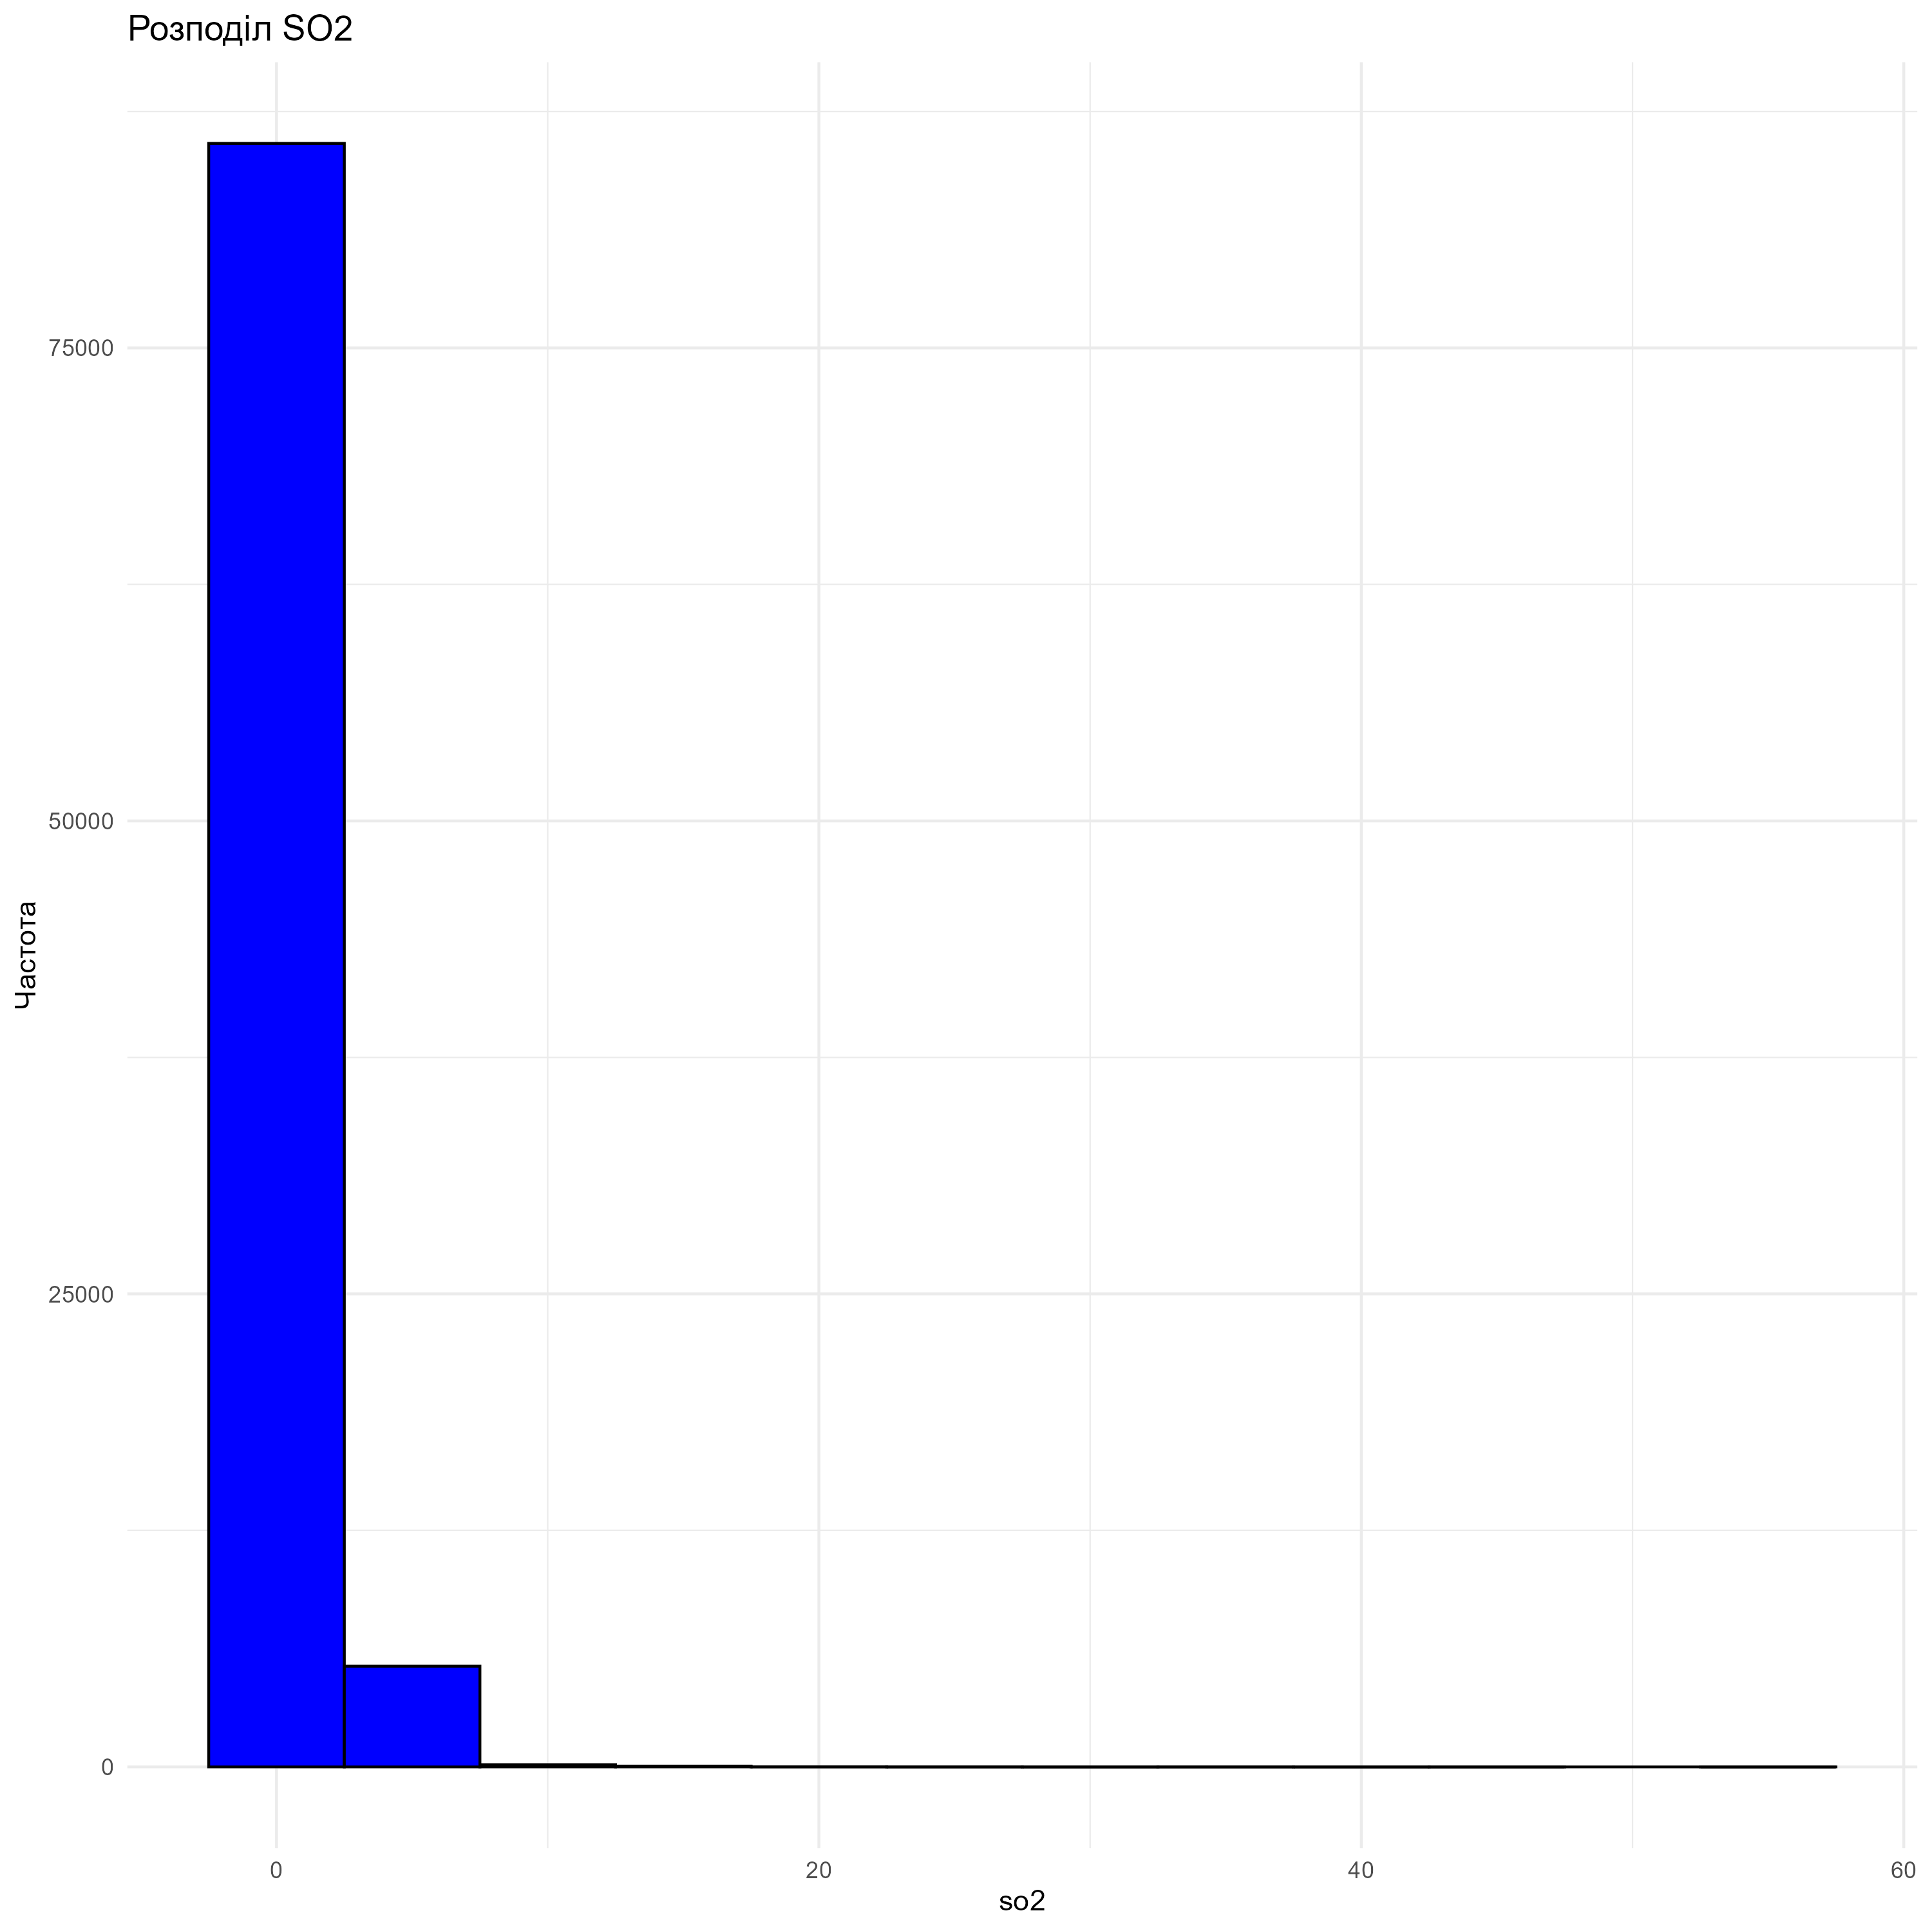
\includegraphics[width=6in]{plots/question2/so2_plot.png}

  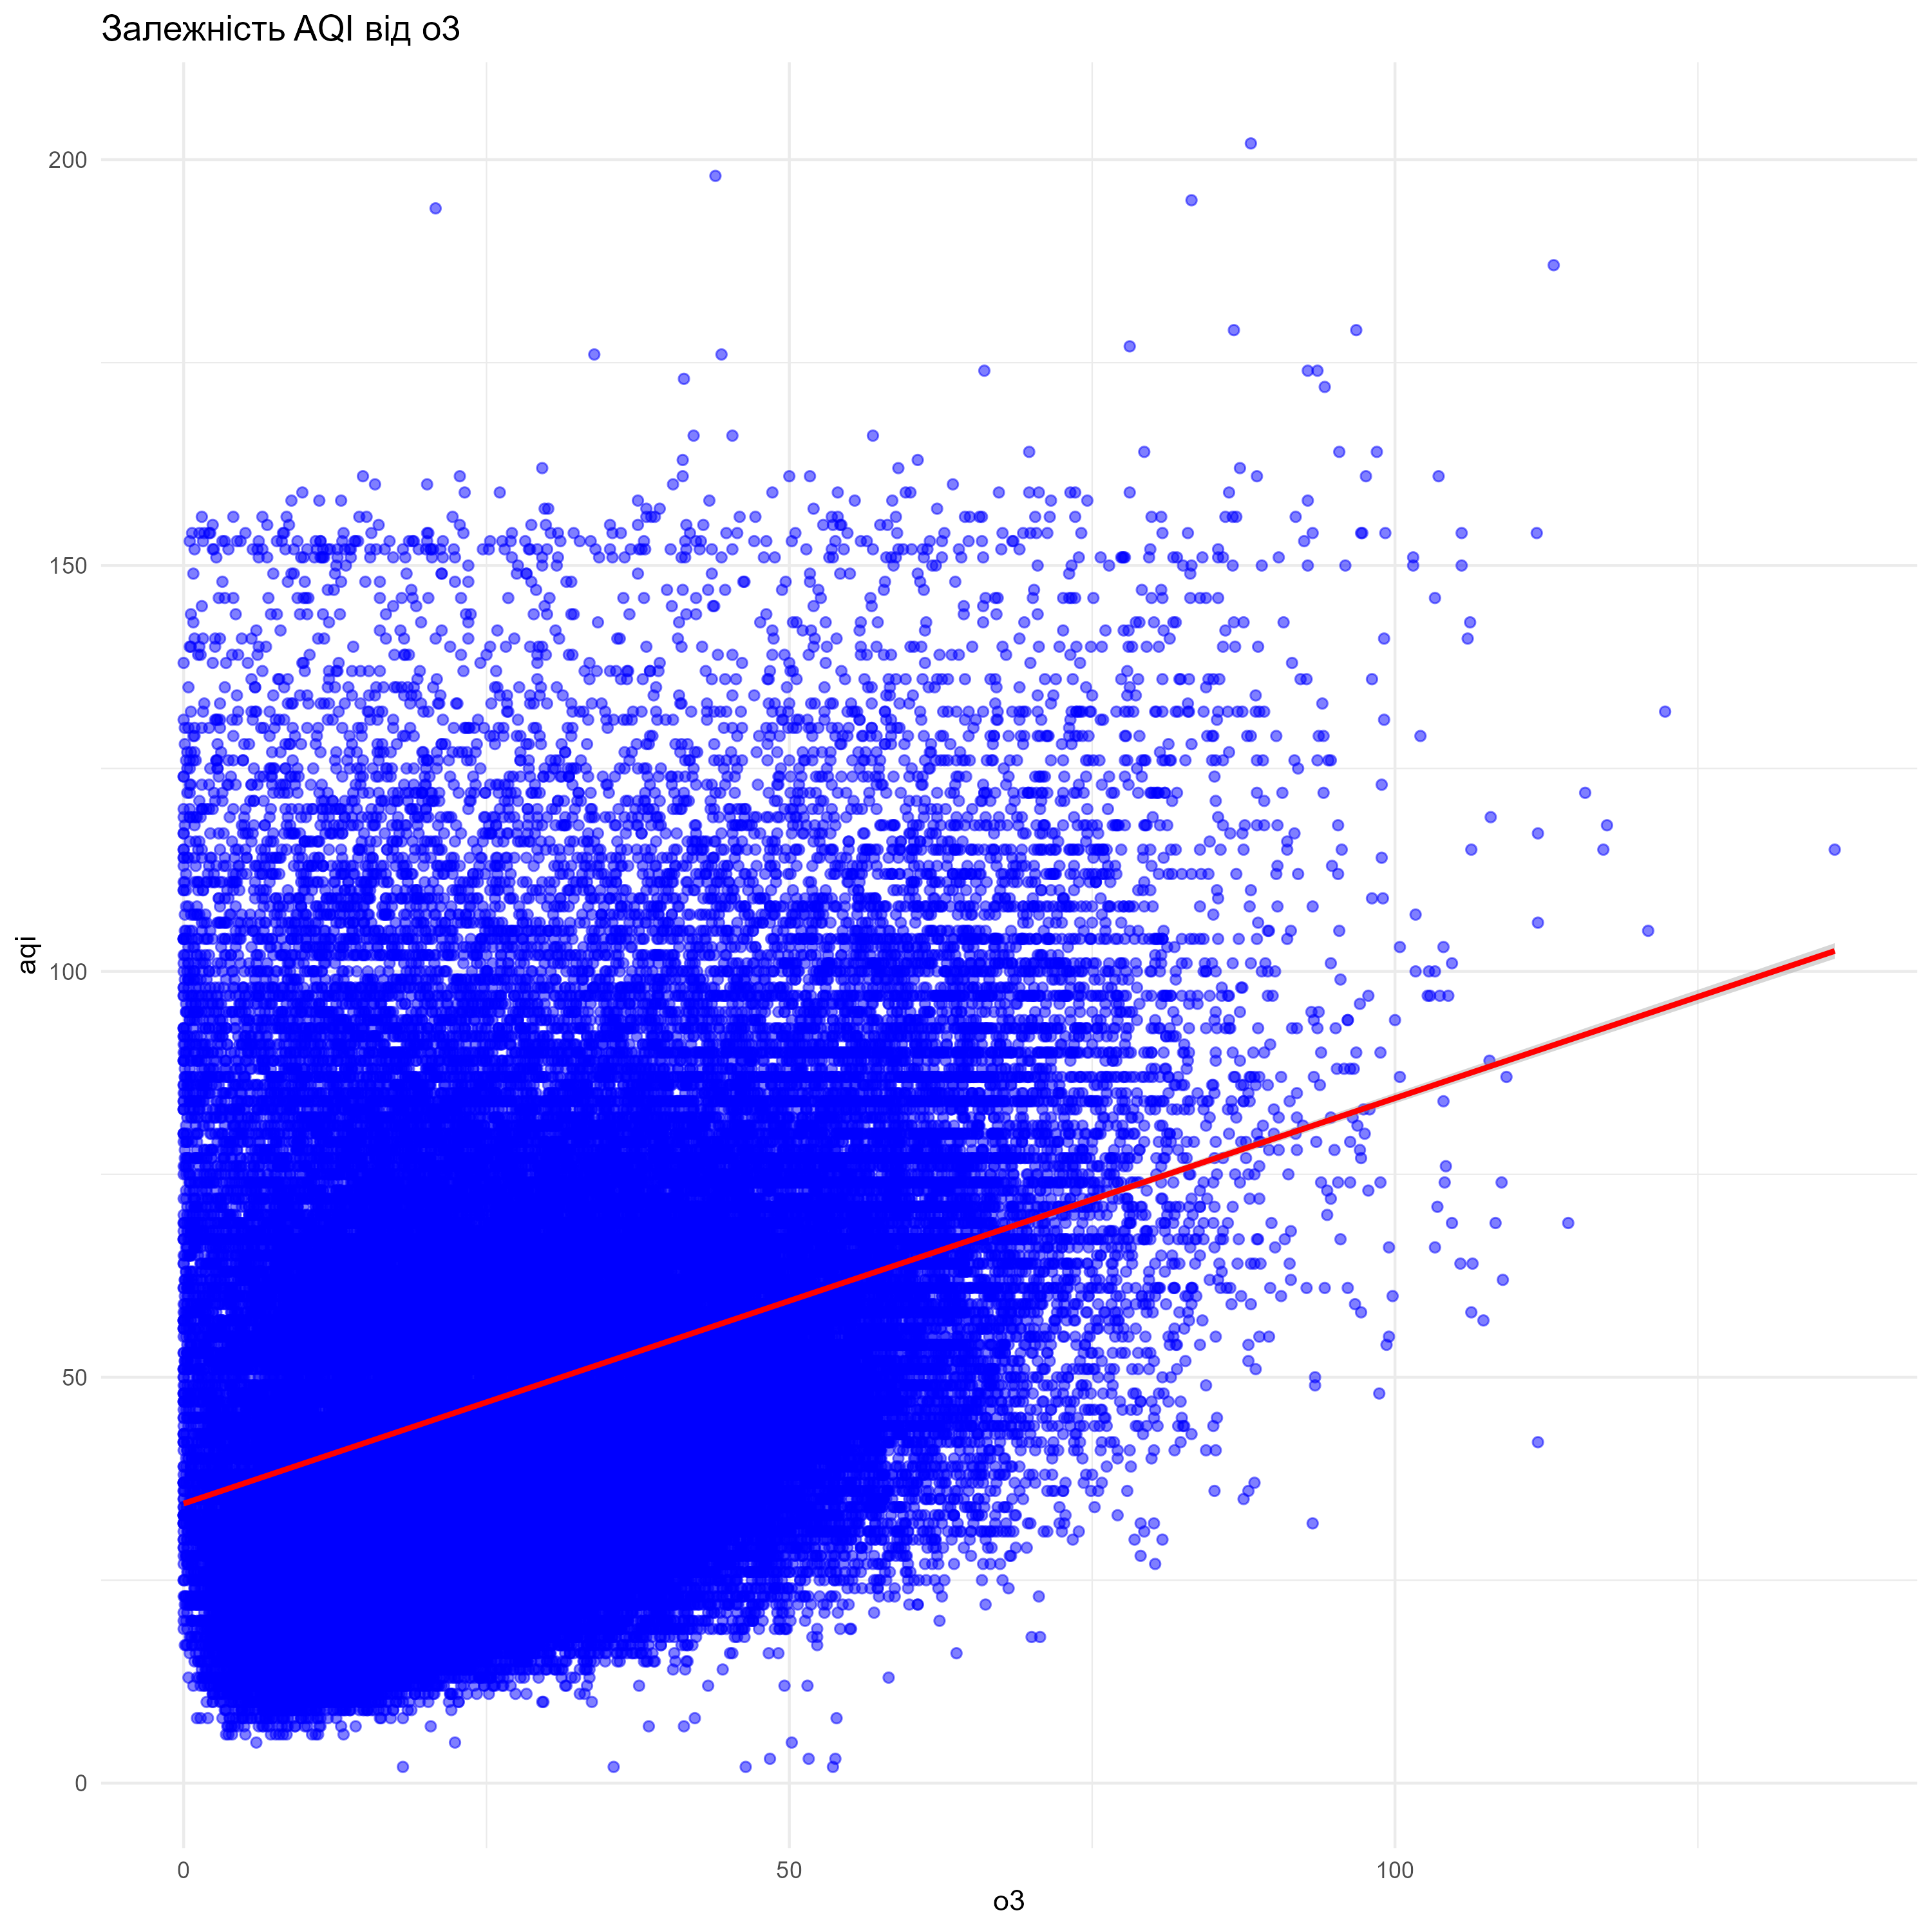
\includegraphics[width=6in]{plots/question2/scatter_plot.png}

  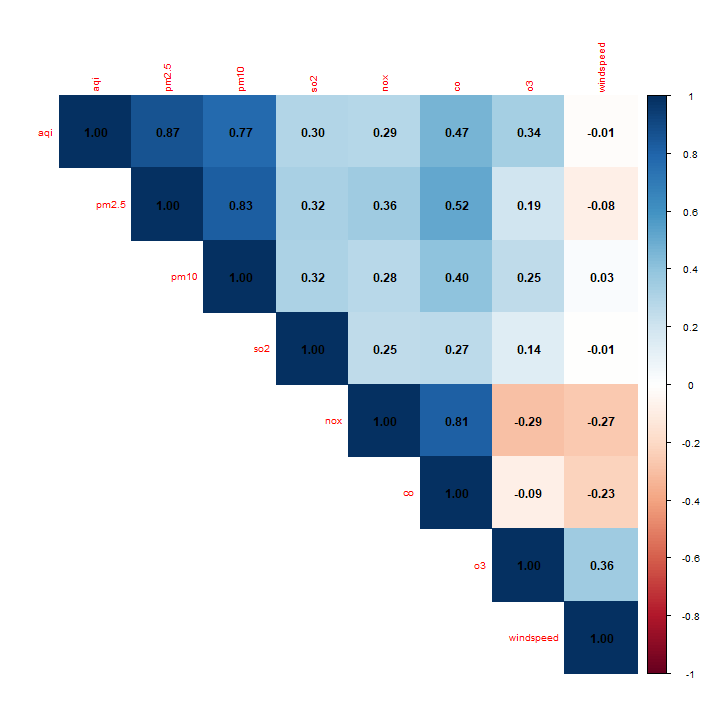
\includegraphics[width=6in]{plots/question2/air_corr_matrix.png}
    
  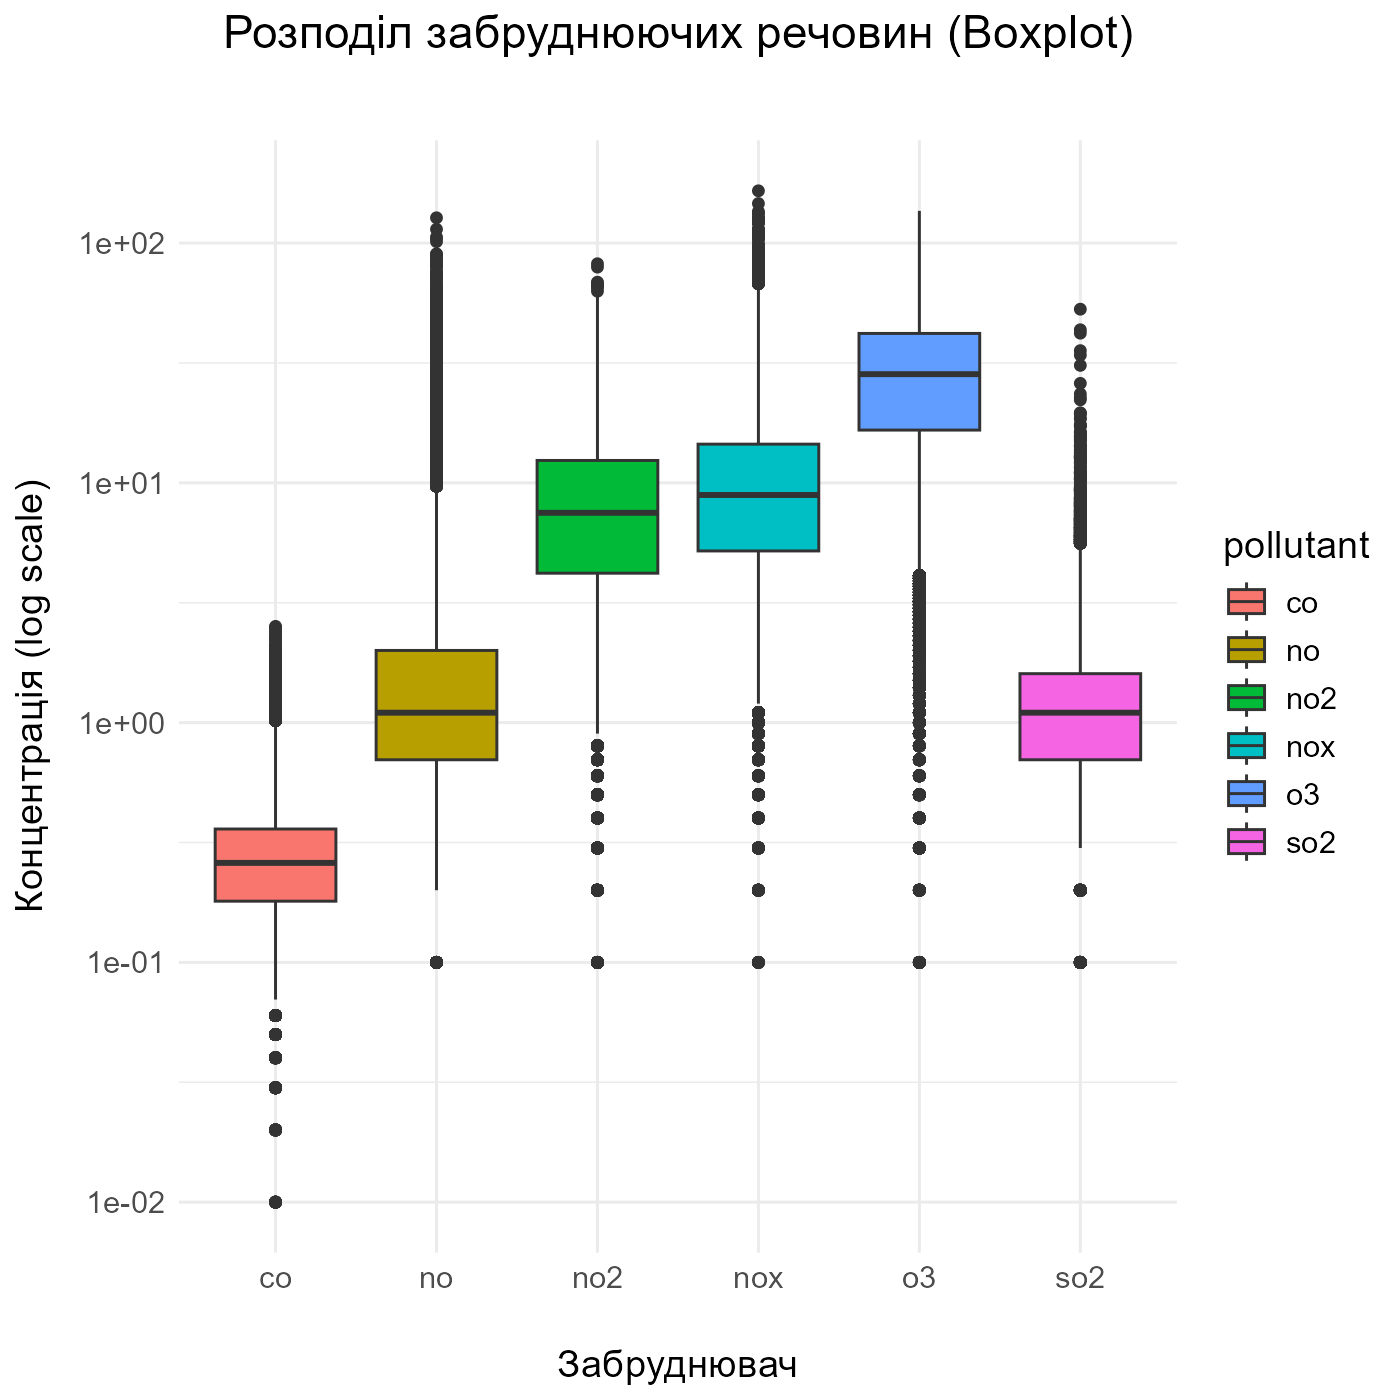
\includegraphics[width=6in]{plots/question2/boxplot_pollutants.png}
    
  \item Як змінюється якість повітря (status) протягом доби в різних районах?
    
  \quad \textit{Був використаний tidy набір даних}

  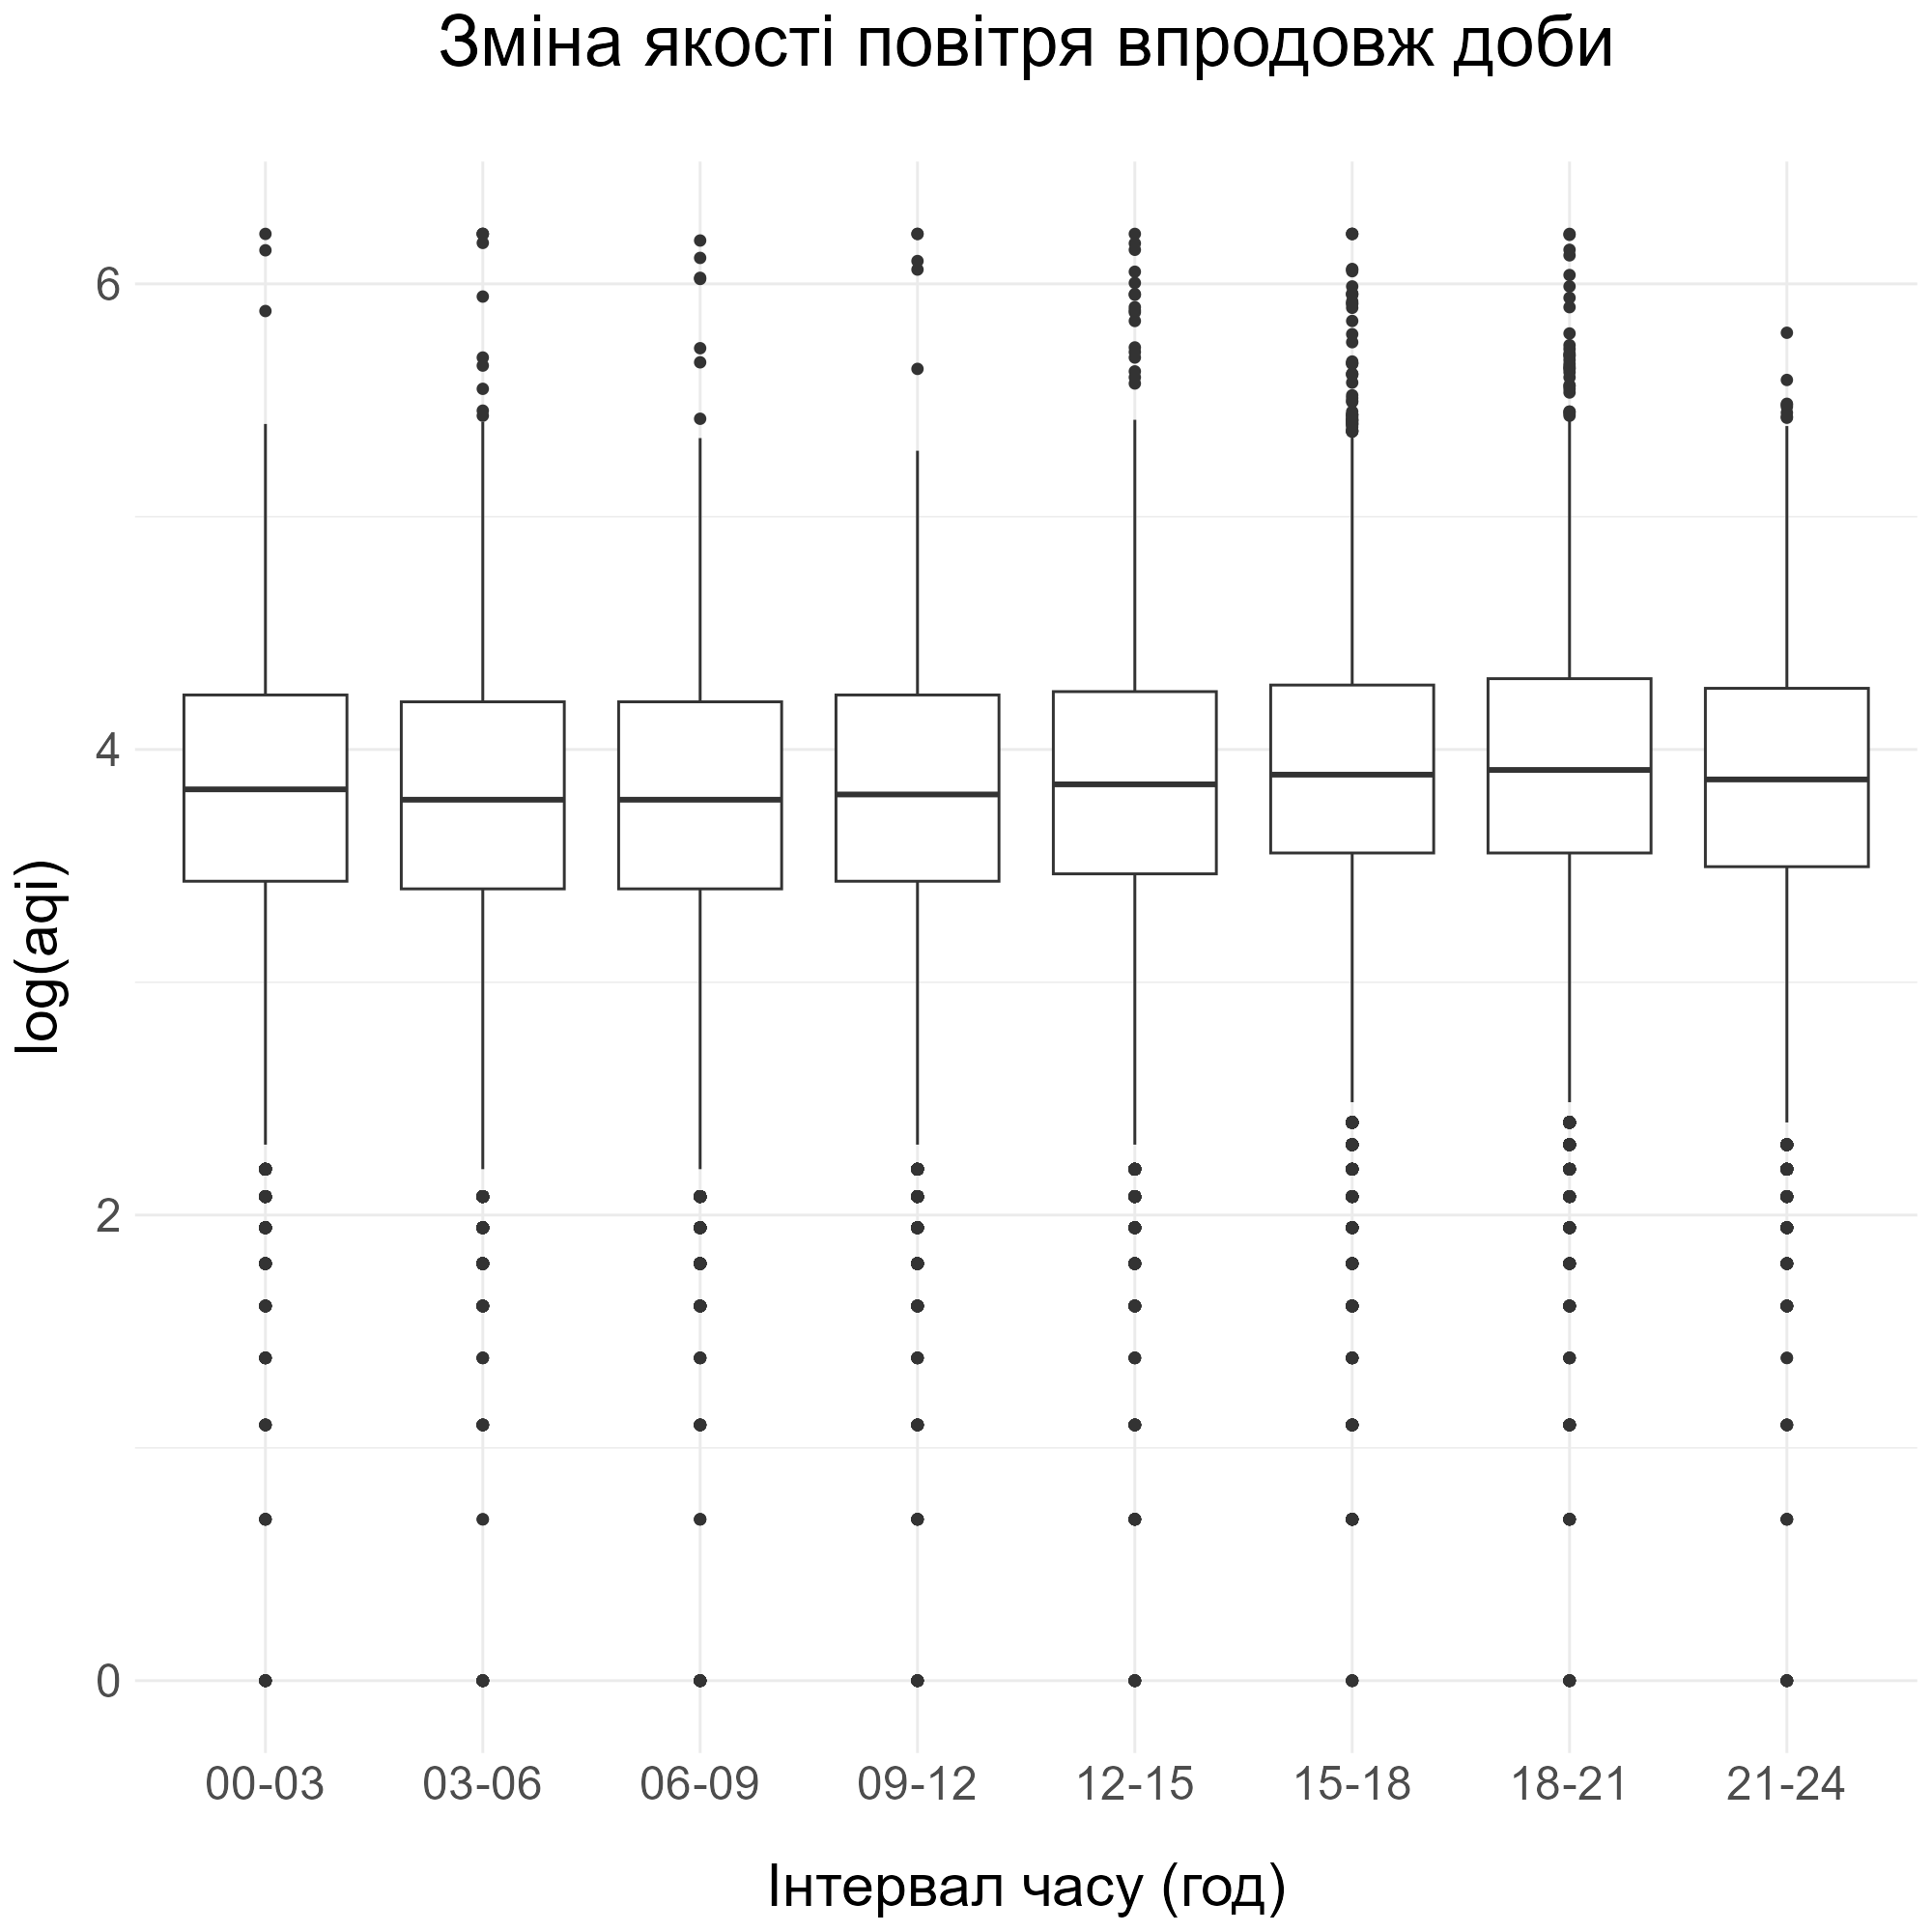
\includegraphics[width=6in]{plots/question3/box.png}
  Аналізуючи даний графік, можна стверджувтаи,що якість повітря трохи покращується у другій половині дня.
    
  Також можемо розглянути детальніше декілкьа регіонів та зміни якости повітря. 

  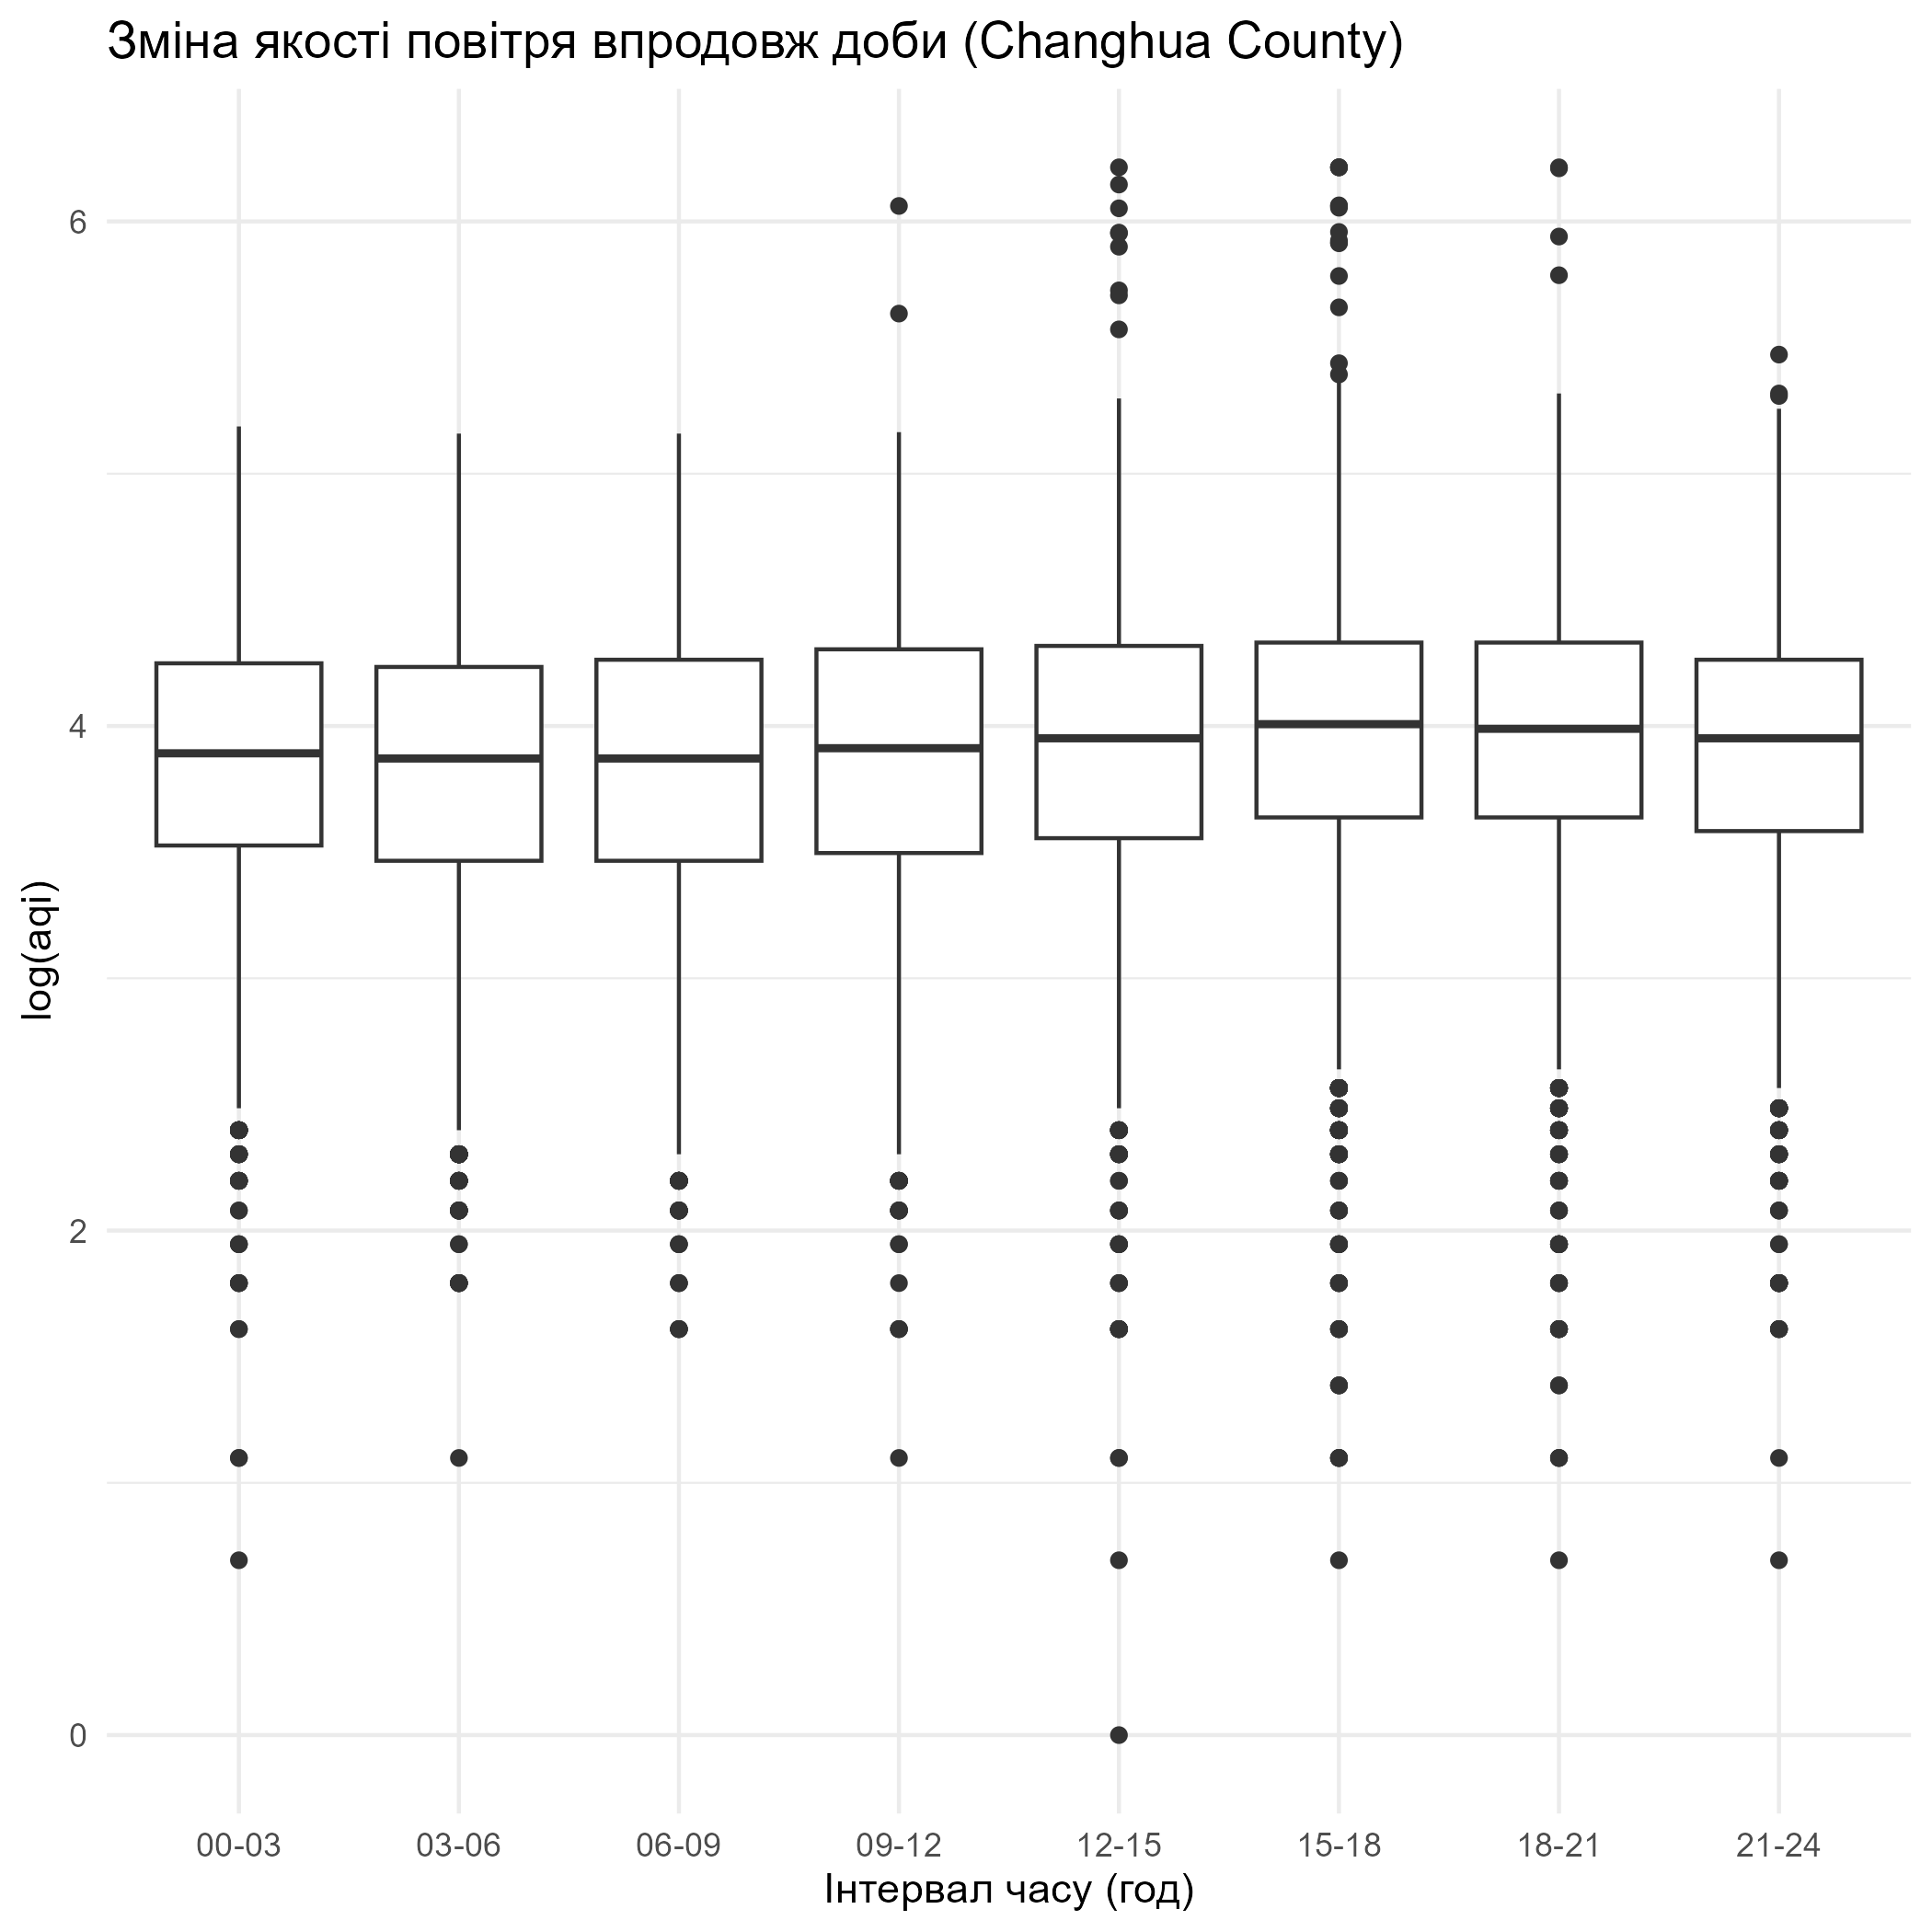
\includegraphics[width=6in]{plots/question3/county-box/Changhua County.png}

  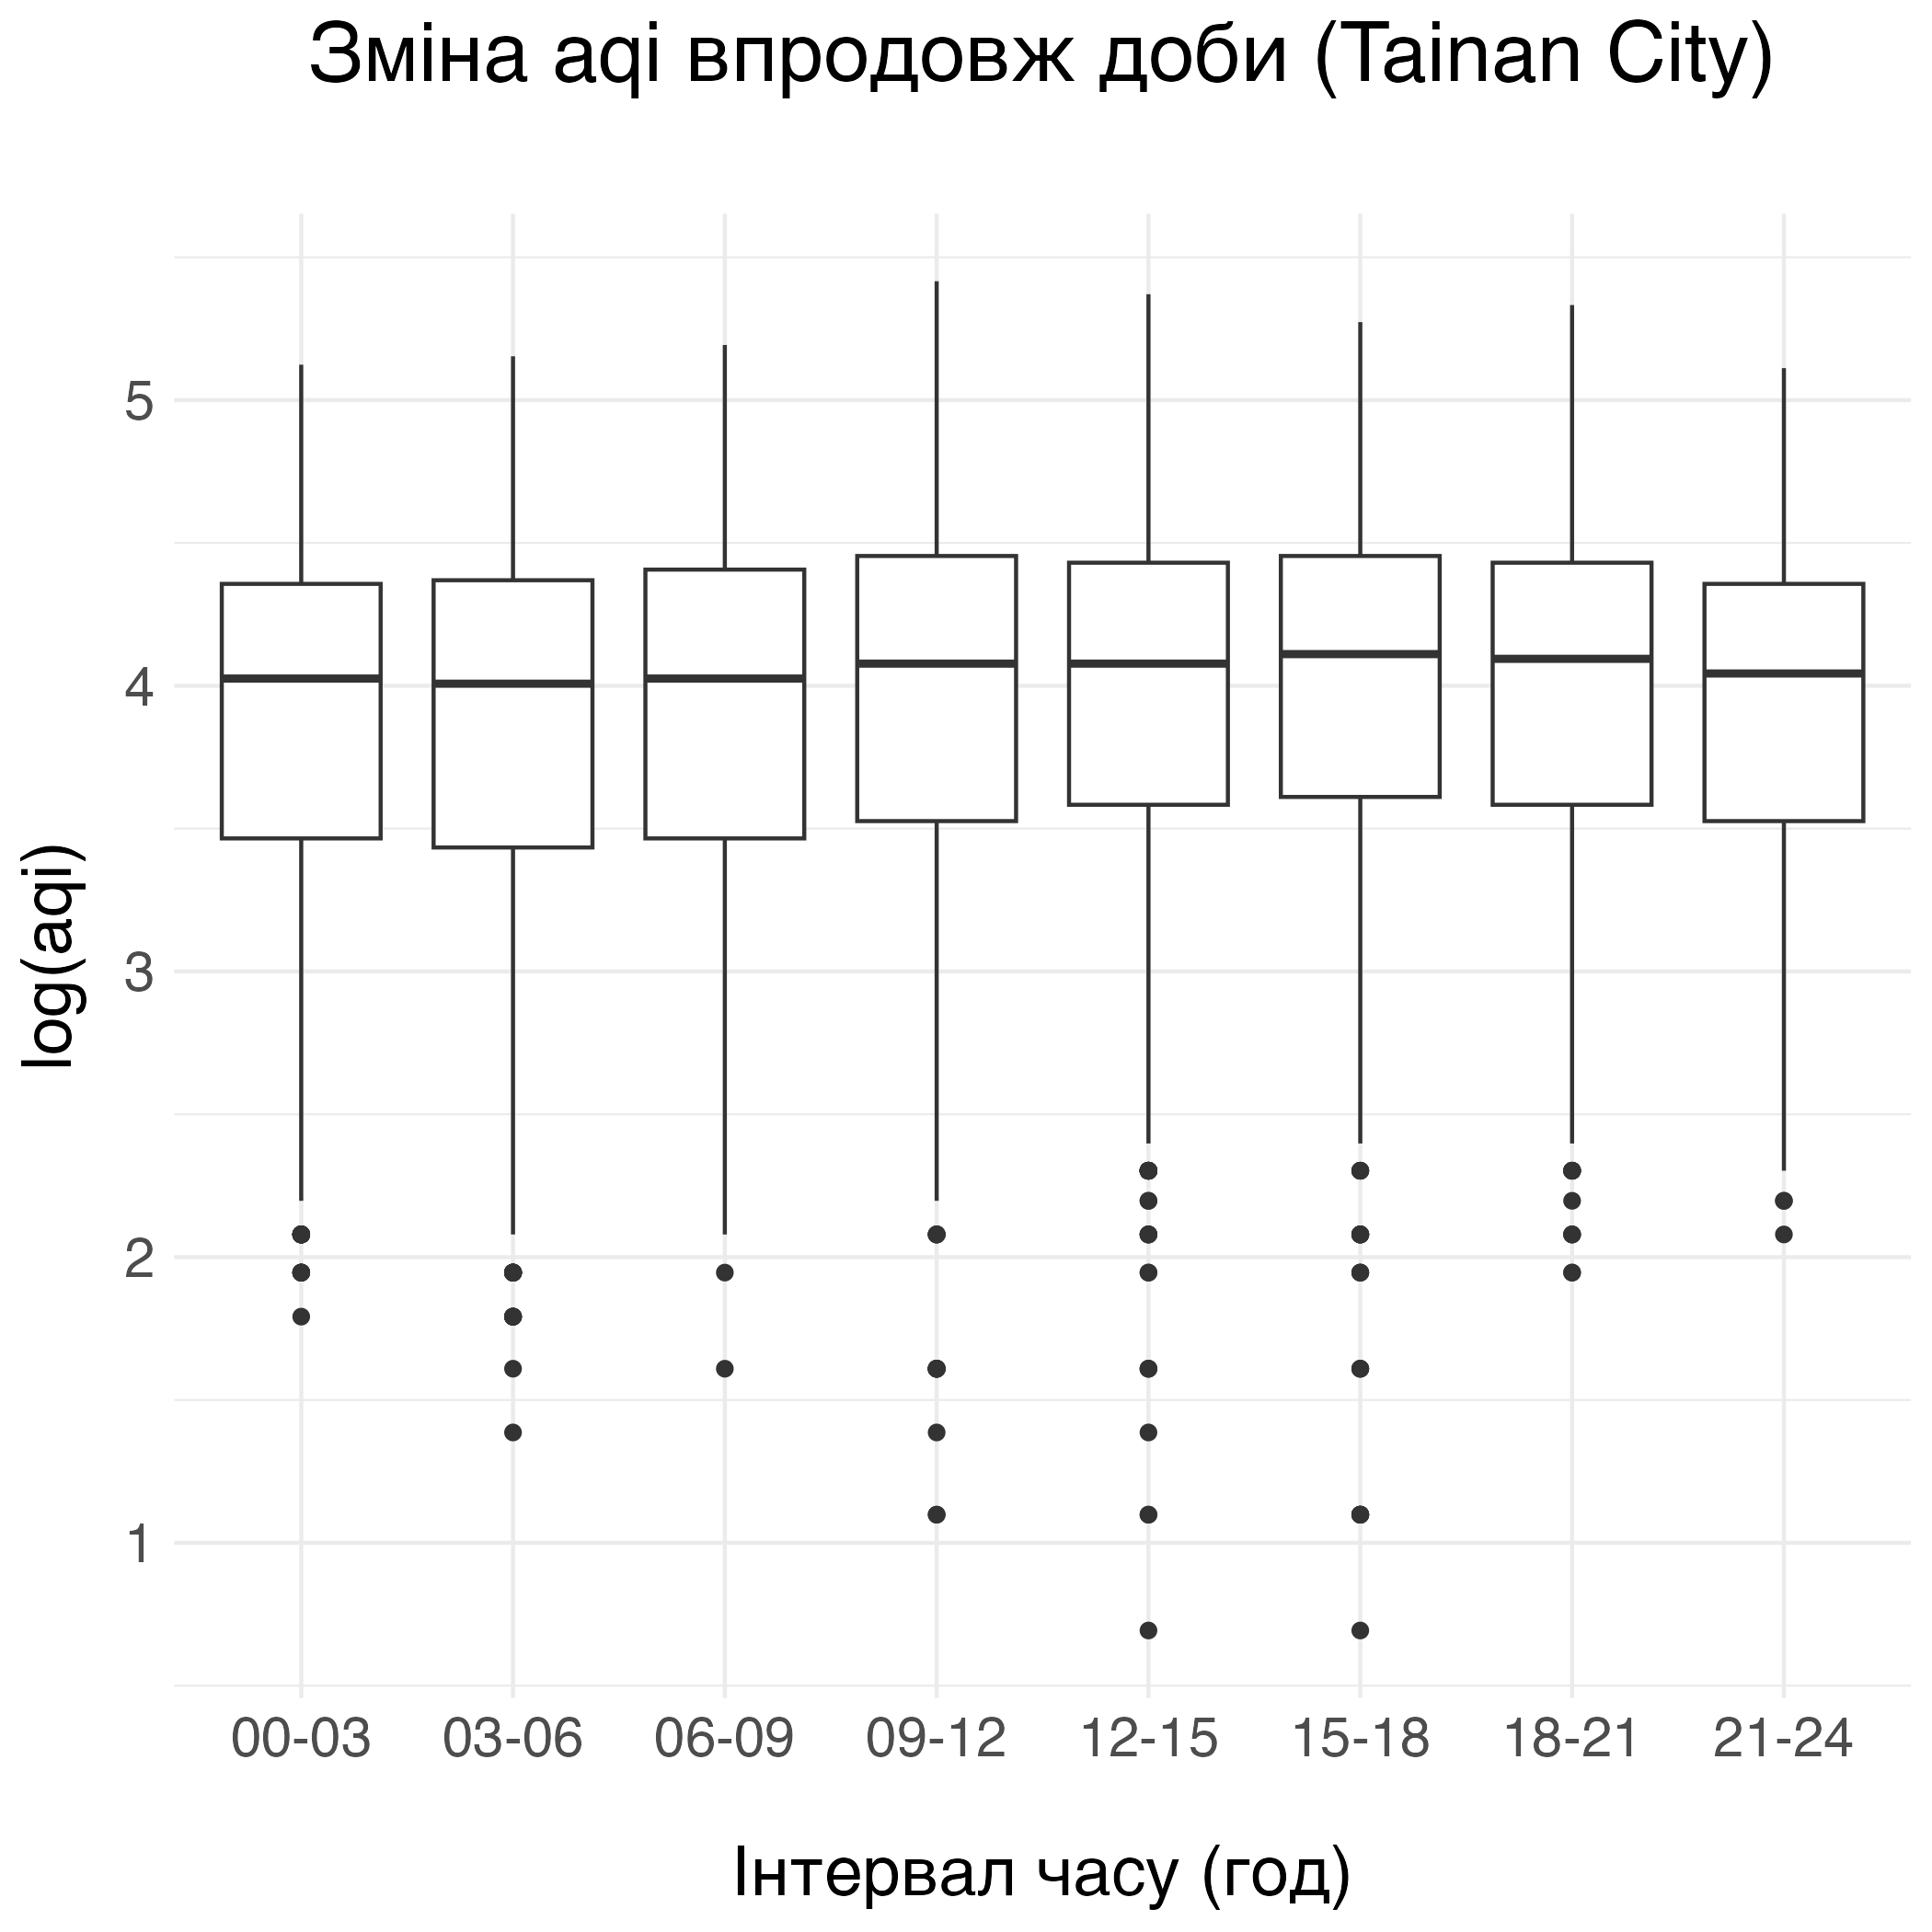
\includegraphics[width=6in]{plots/question3/county-box/Tainan City.png}

  Бачимо, що 

  \item Які регіони (county) мають найвищий середній рівень забруднення повітря (AQI) протягом року?
    
  \quad \textit{Був використаний trimmed набір даних}

  Всі наступні графіки, будуть будуватися на основі даних за 2016, 2017, 2023 та 2024 роки.
    
  Для розуміння числових даних, розглянемо 10 регіонів з найвищим рівнем AQI за відповідні роки.
    
  \begin{tabular}{ccc}
    \textbf{Year} & \textbf{Сounty} \\ \textbf{avg\_AQI}
    2016 &      Chiayi City & 120.31 \\
    2016 &  Kaohsiung City  & 112.10 \\
    2016 &      Tainan City &  99.60 \\
    2016 &  Pingtung County &  97.15 \\
    2016 &   Yunlin County  &  91.23 \\
    2016 &   Chiayi County  &  88.83 \\
    2016 &   Nantou County  &  83.34 \\
    2016 & Changhua County  &  81.68 \\
    2016 &   Kinmen County  &  81.60 \\
    2016 &  Taichung City   &  77.96 \\
  \end{tabular}
    
  Візуалізуючи отримуємо наступне:
  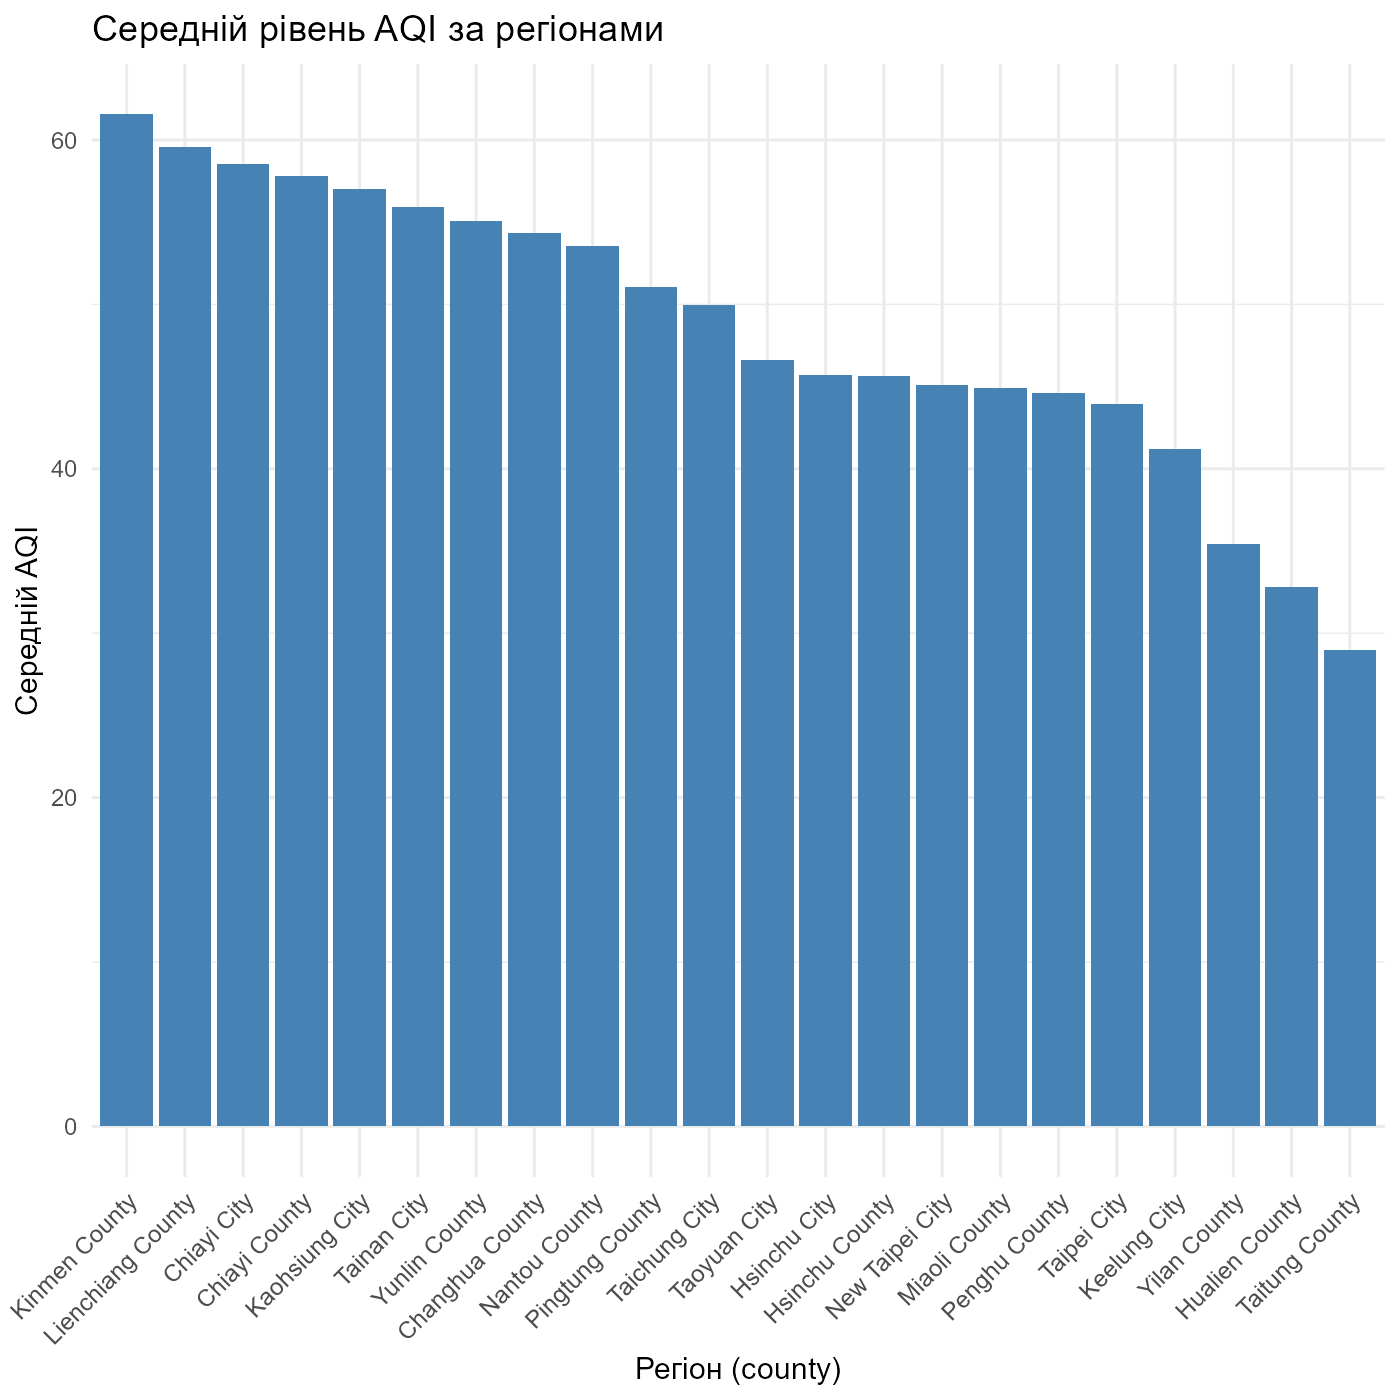
\includegraphics[width=6in]{plots/question4/avg_aqi_by_country.png}
  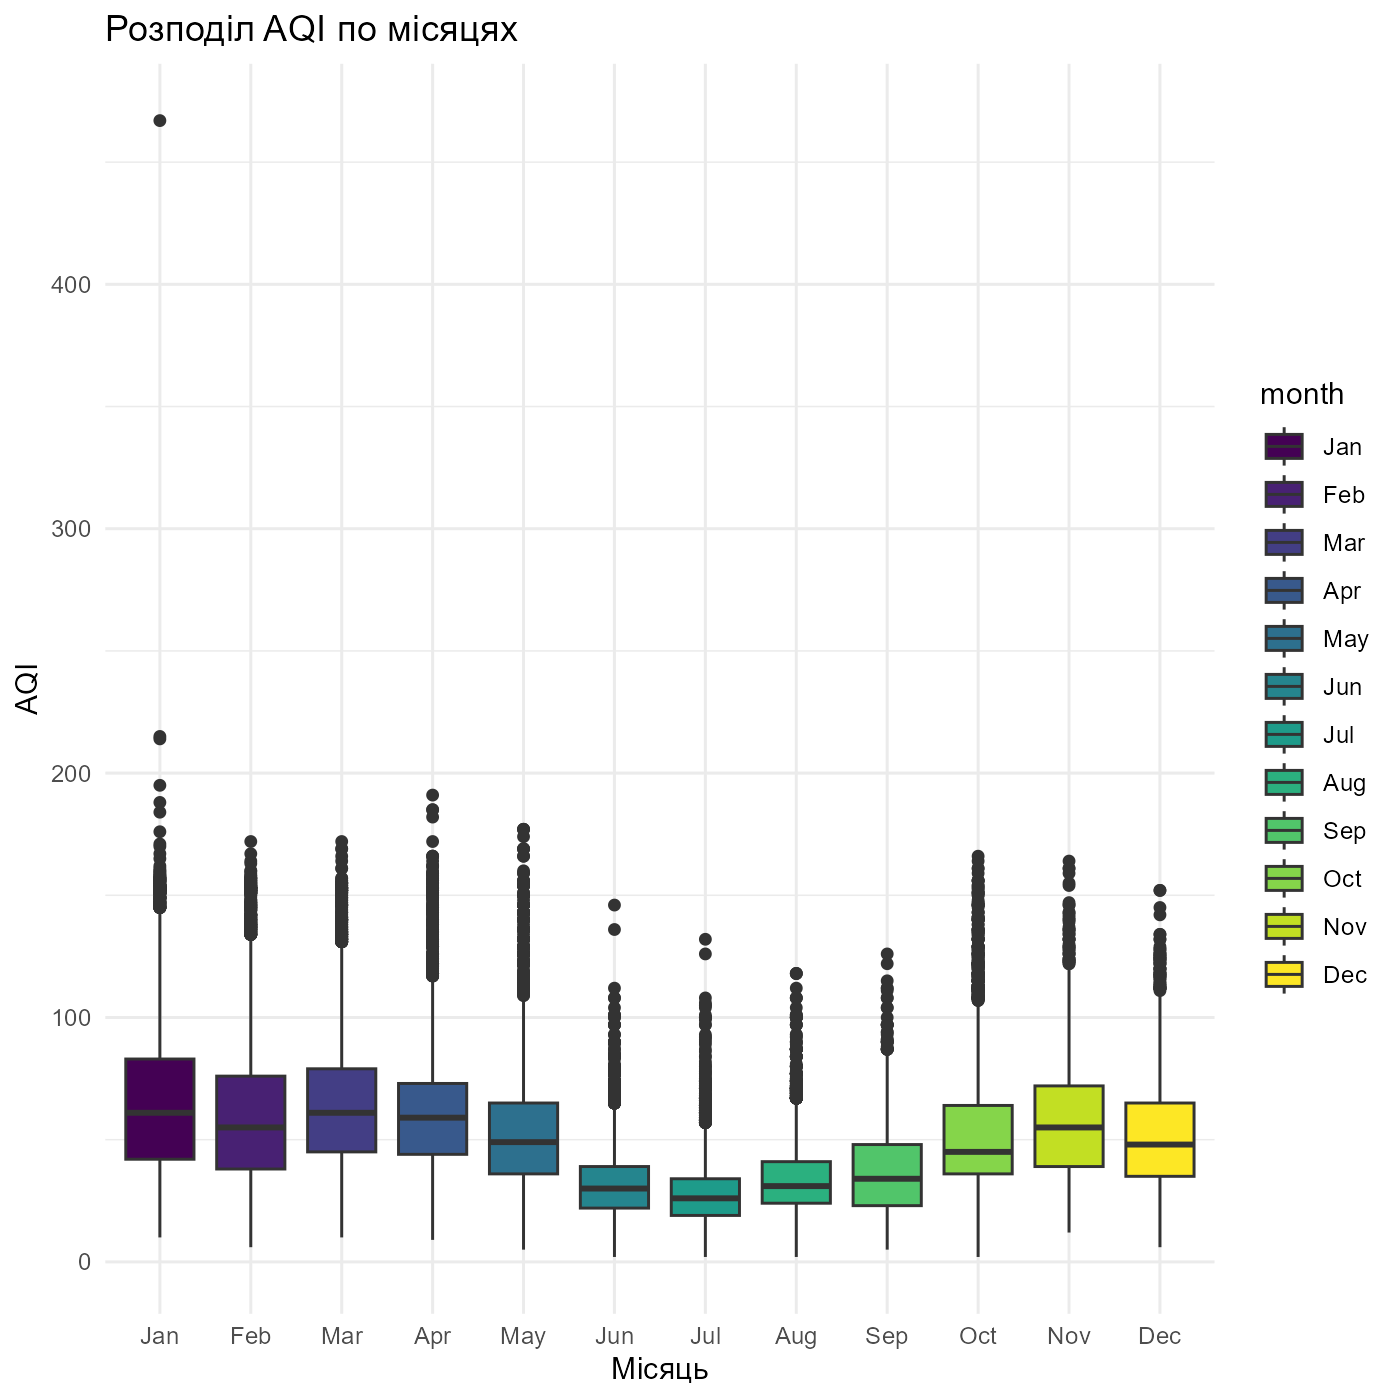
\includegraphics[width=6in]{plots/question4/seasonal_change.png}
    
  \item Як змінився загальний рівень забруднення по регіонам після початку реформи?
    
  \quad \textit{Був використаний tidy набір даних}

  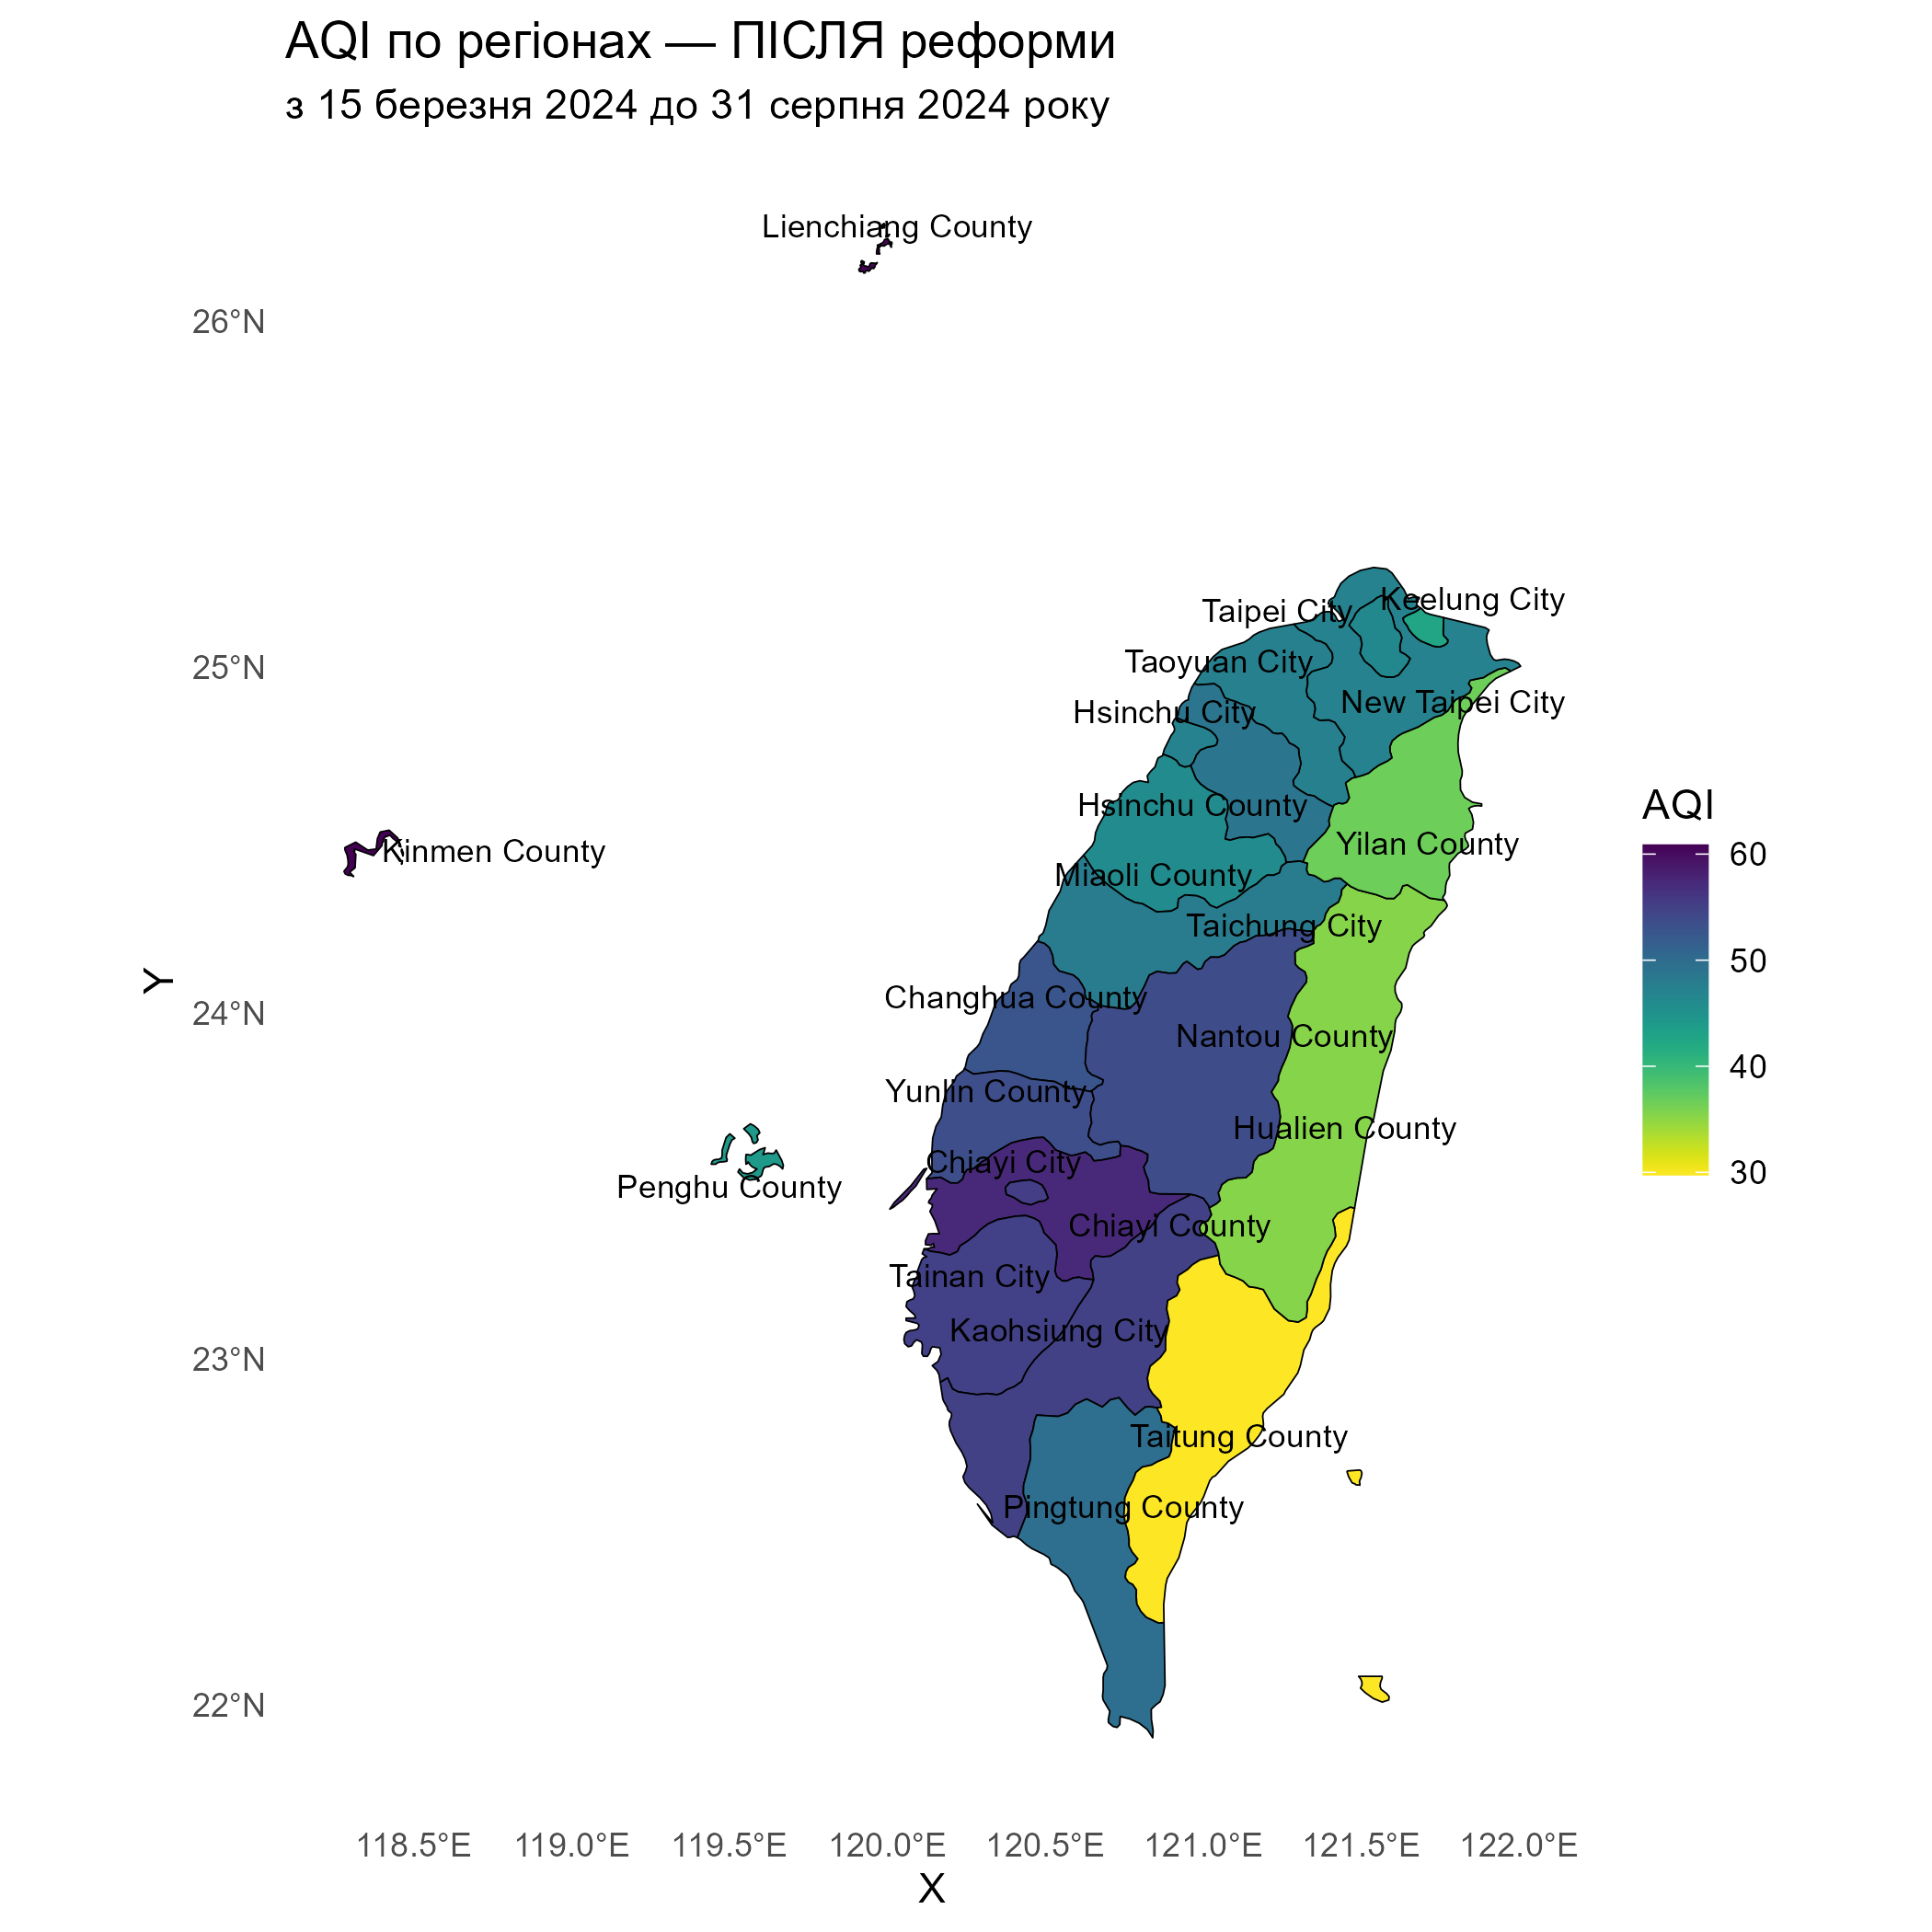
\includegraphics[width=6in]{plots/question5/map_after_reform.png}
  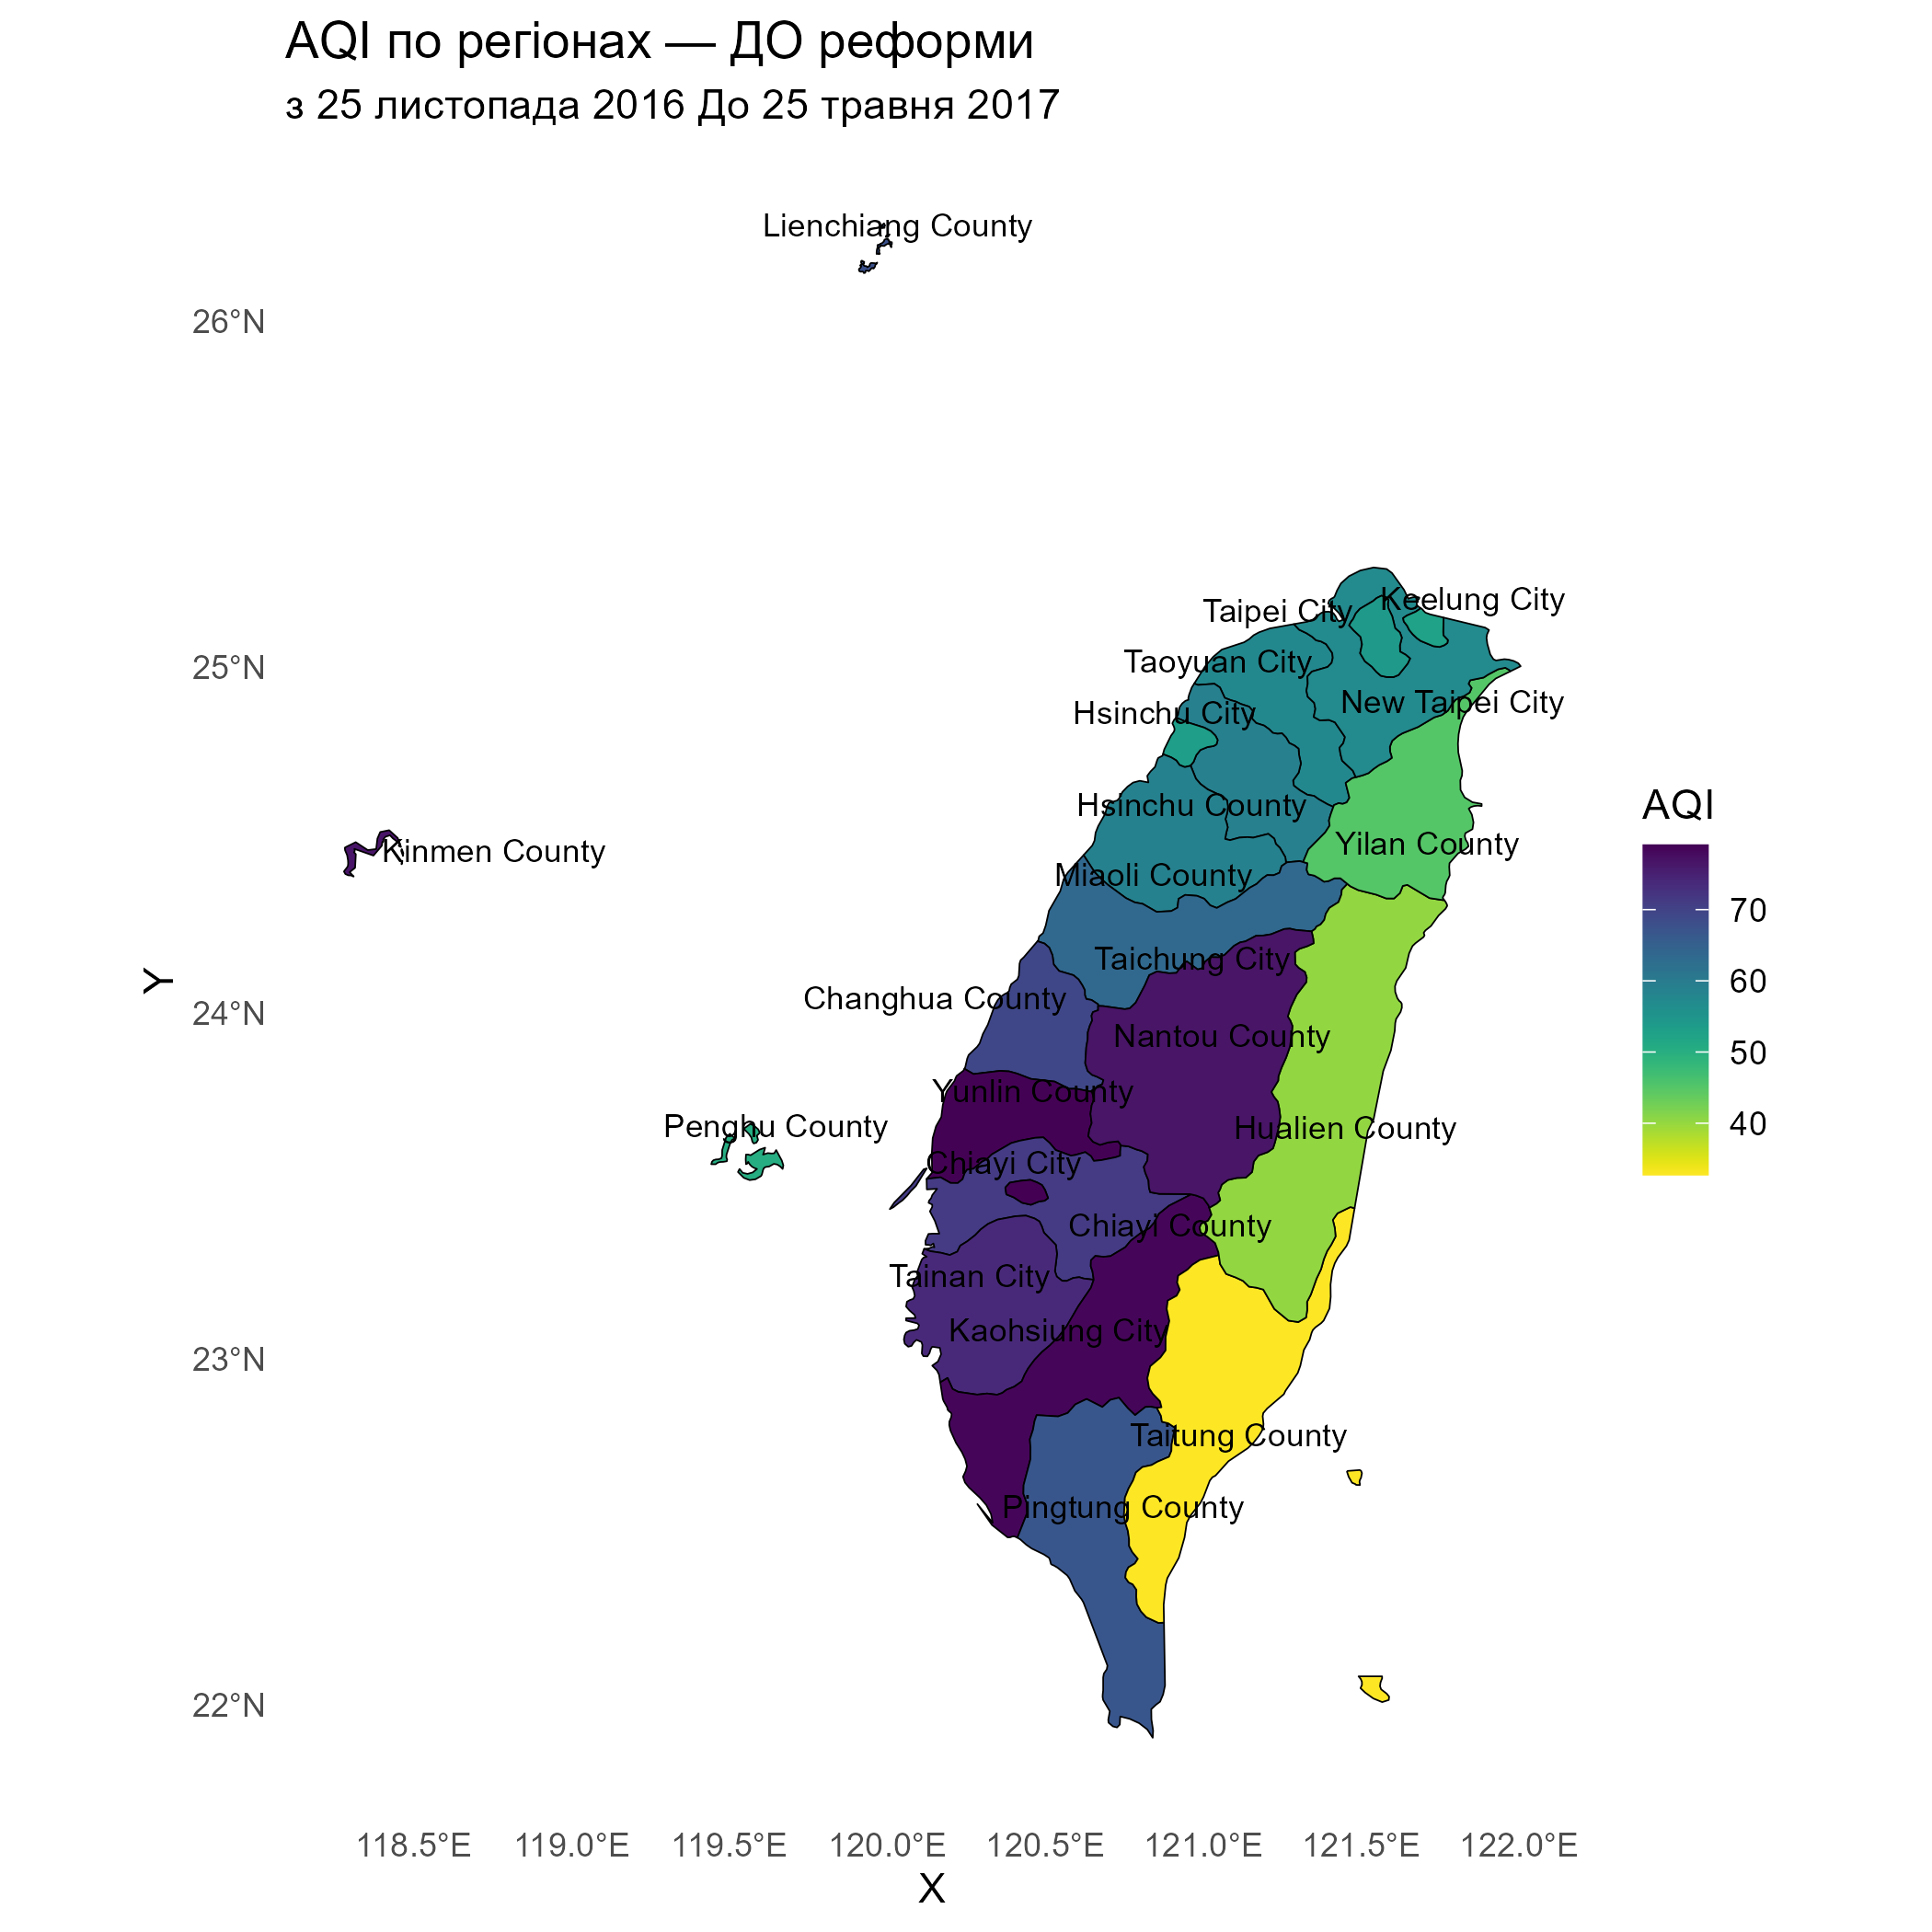
\includegraphics[width=6in]{plots/question5/map_before_reform.png}
  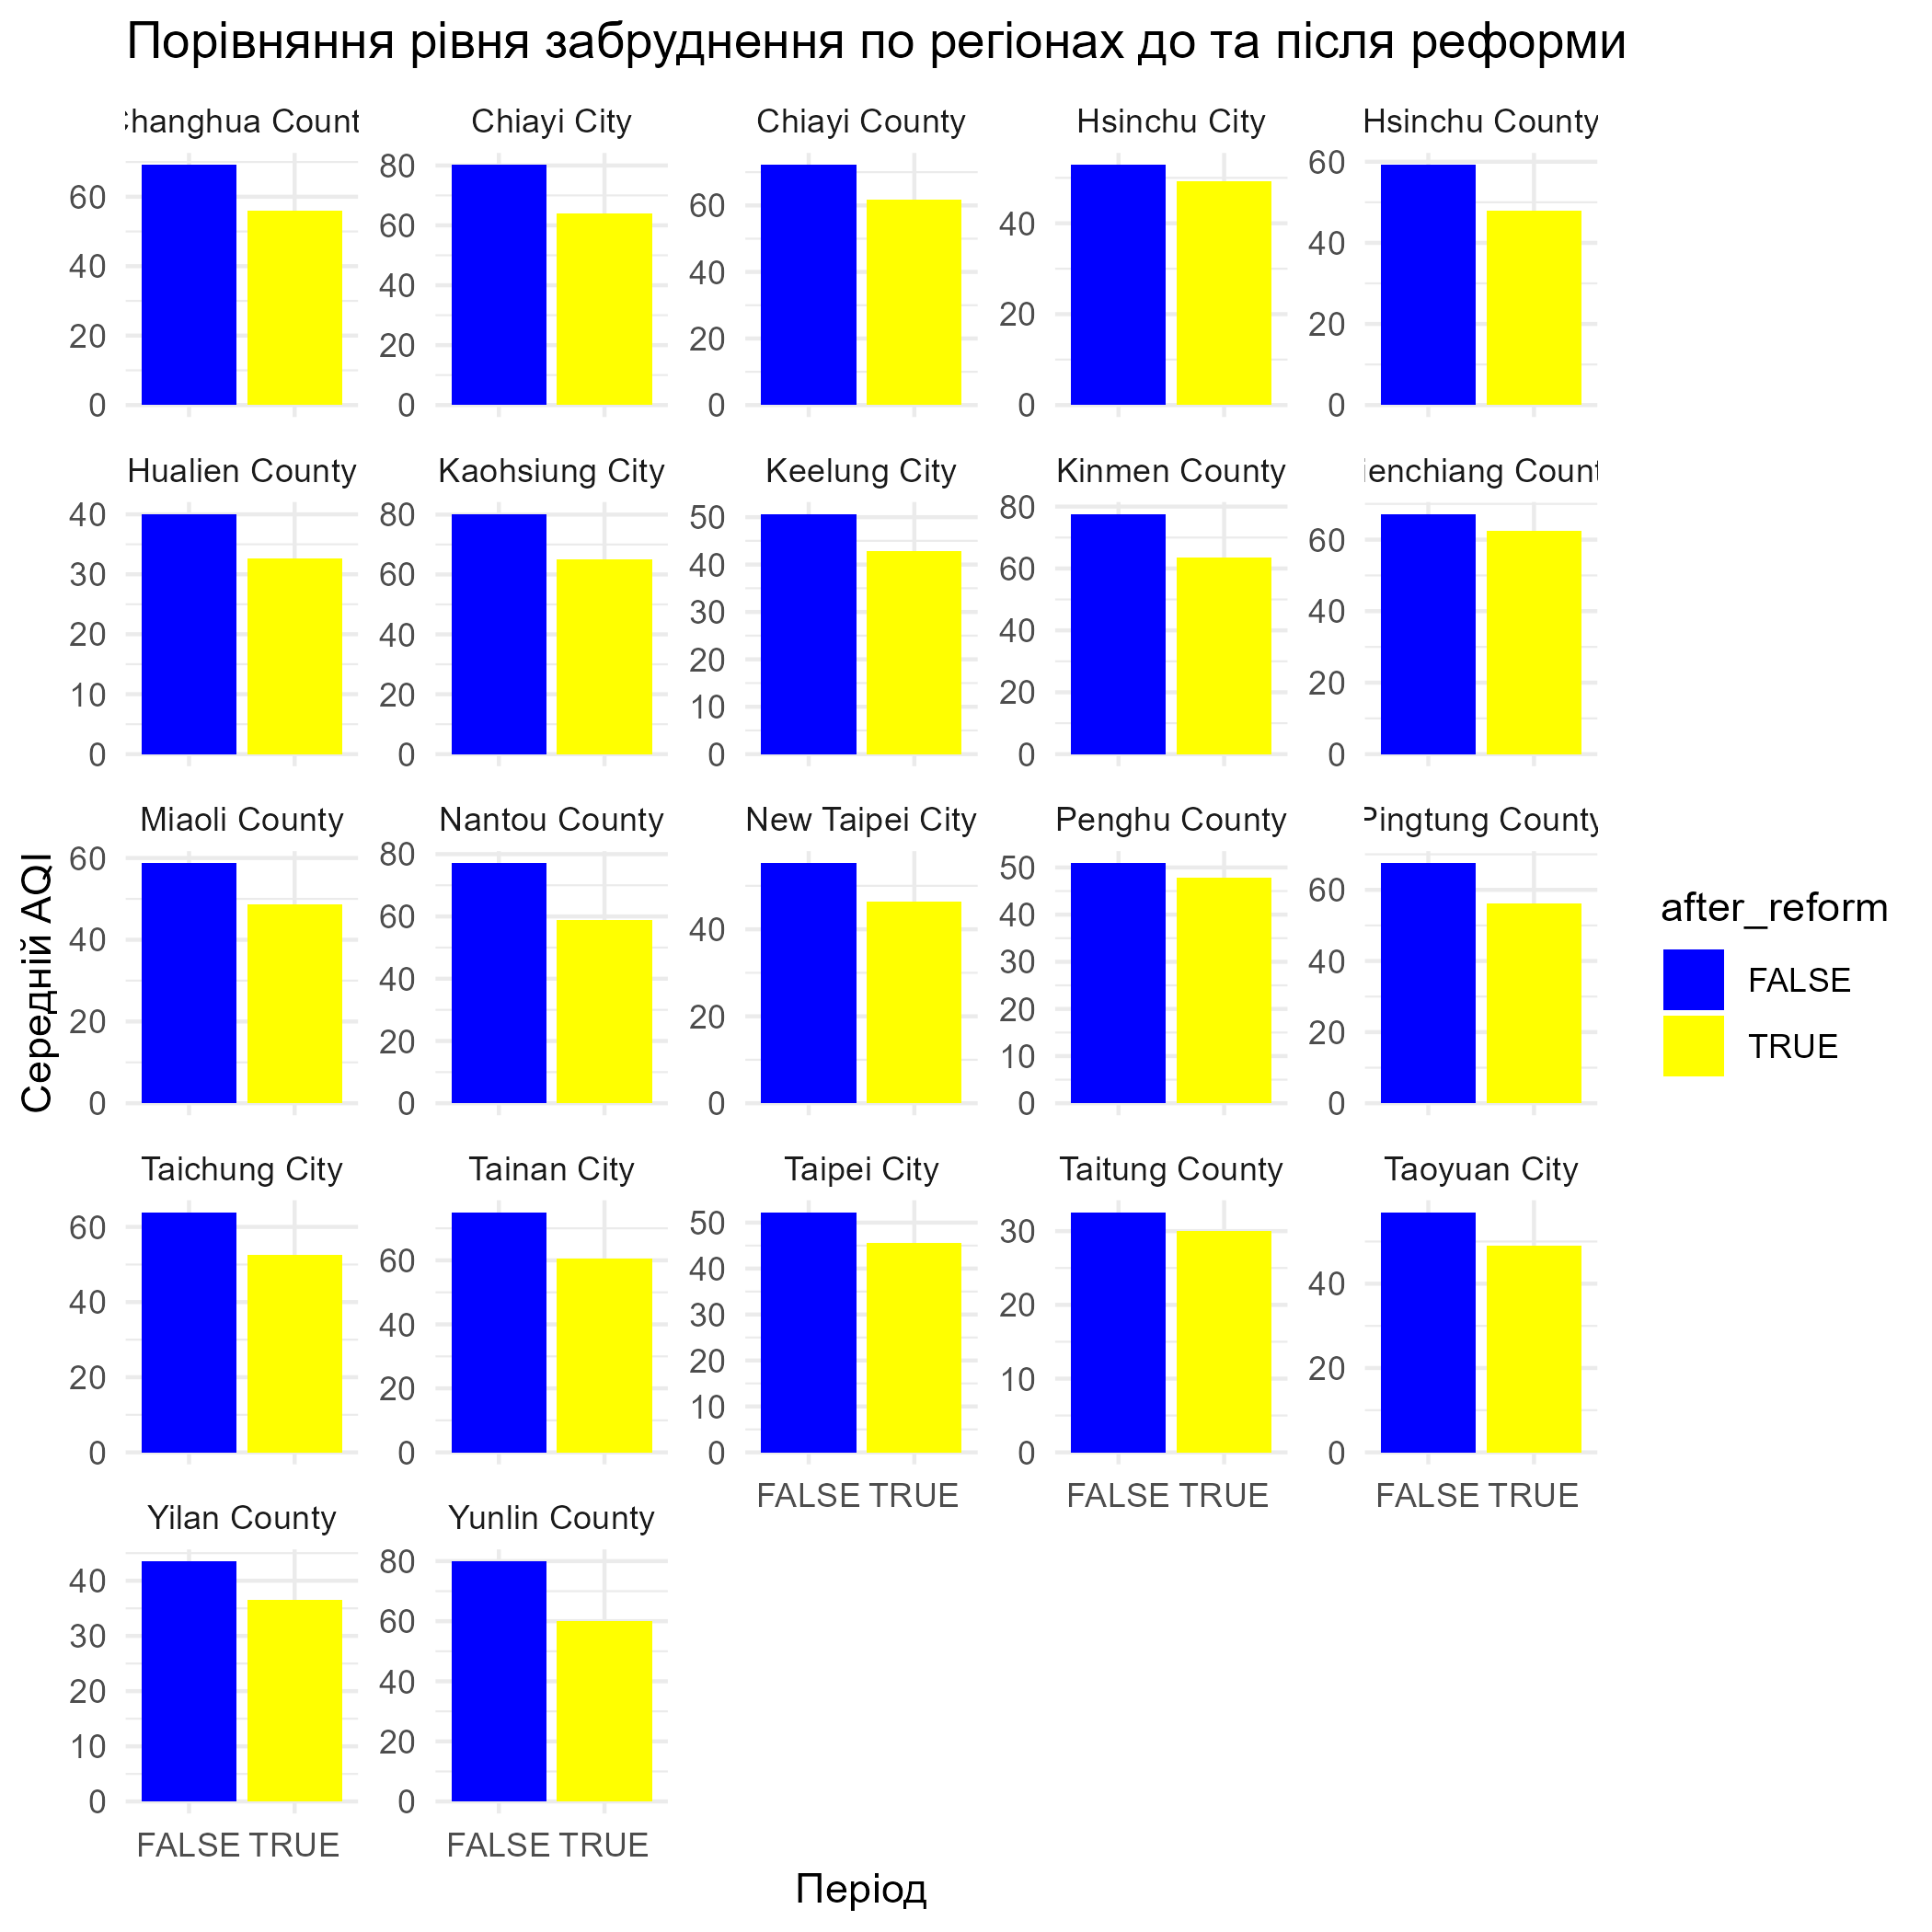
\includegraphics[width=6in]{plots/question5/region_comparison_aqi.png}
    
  \item Чи існує залежність між початком реформ та показниками забруднення?
    
  \quad \textit{Був використаний tidy набір даних}

  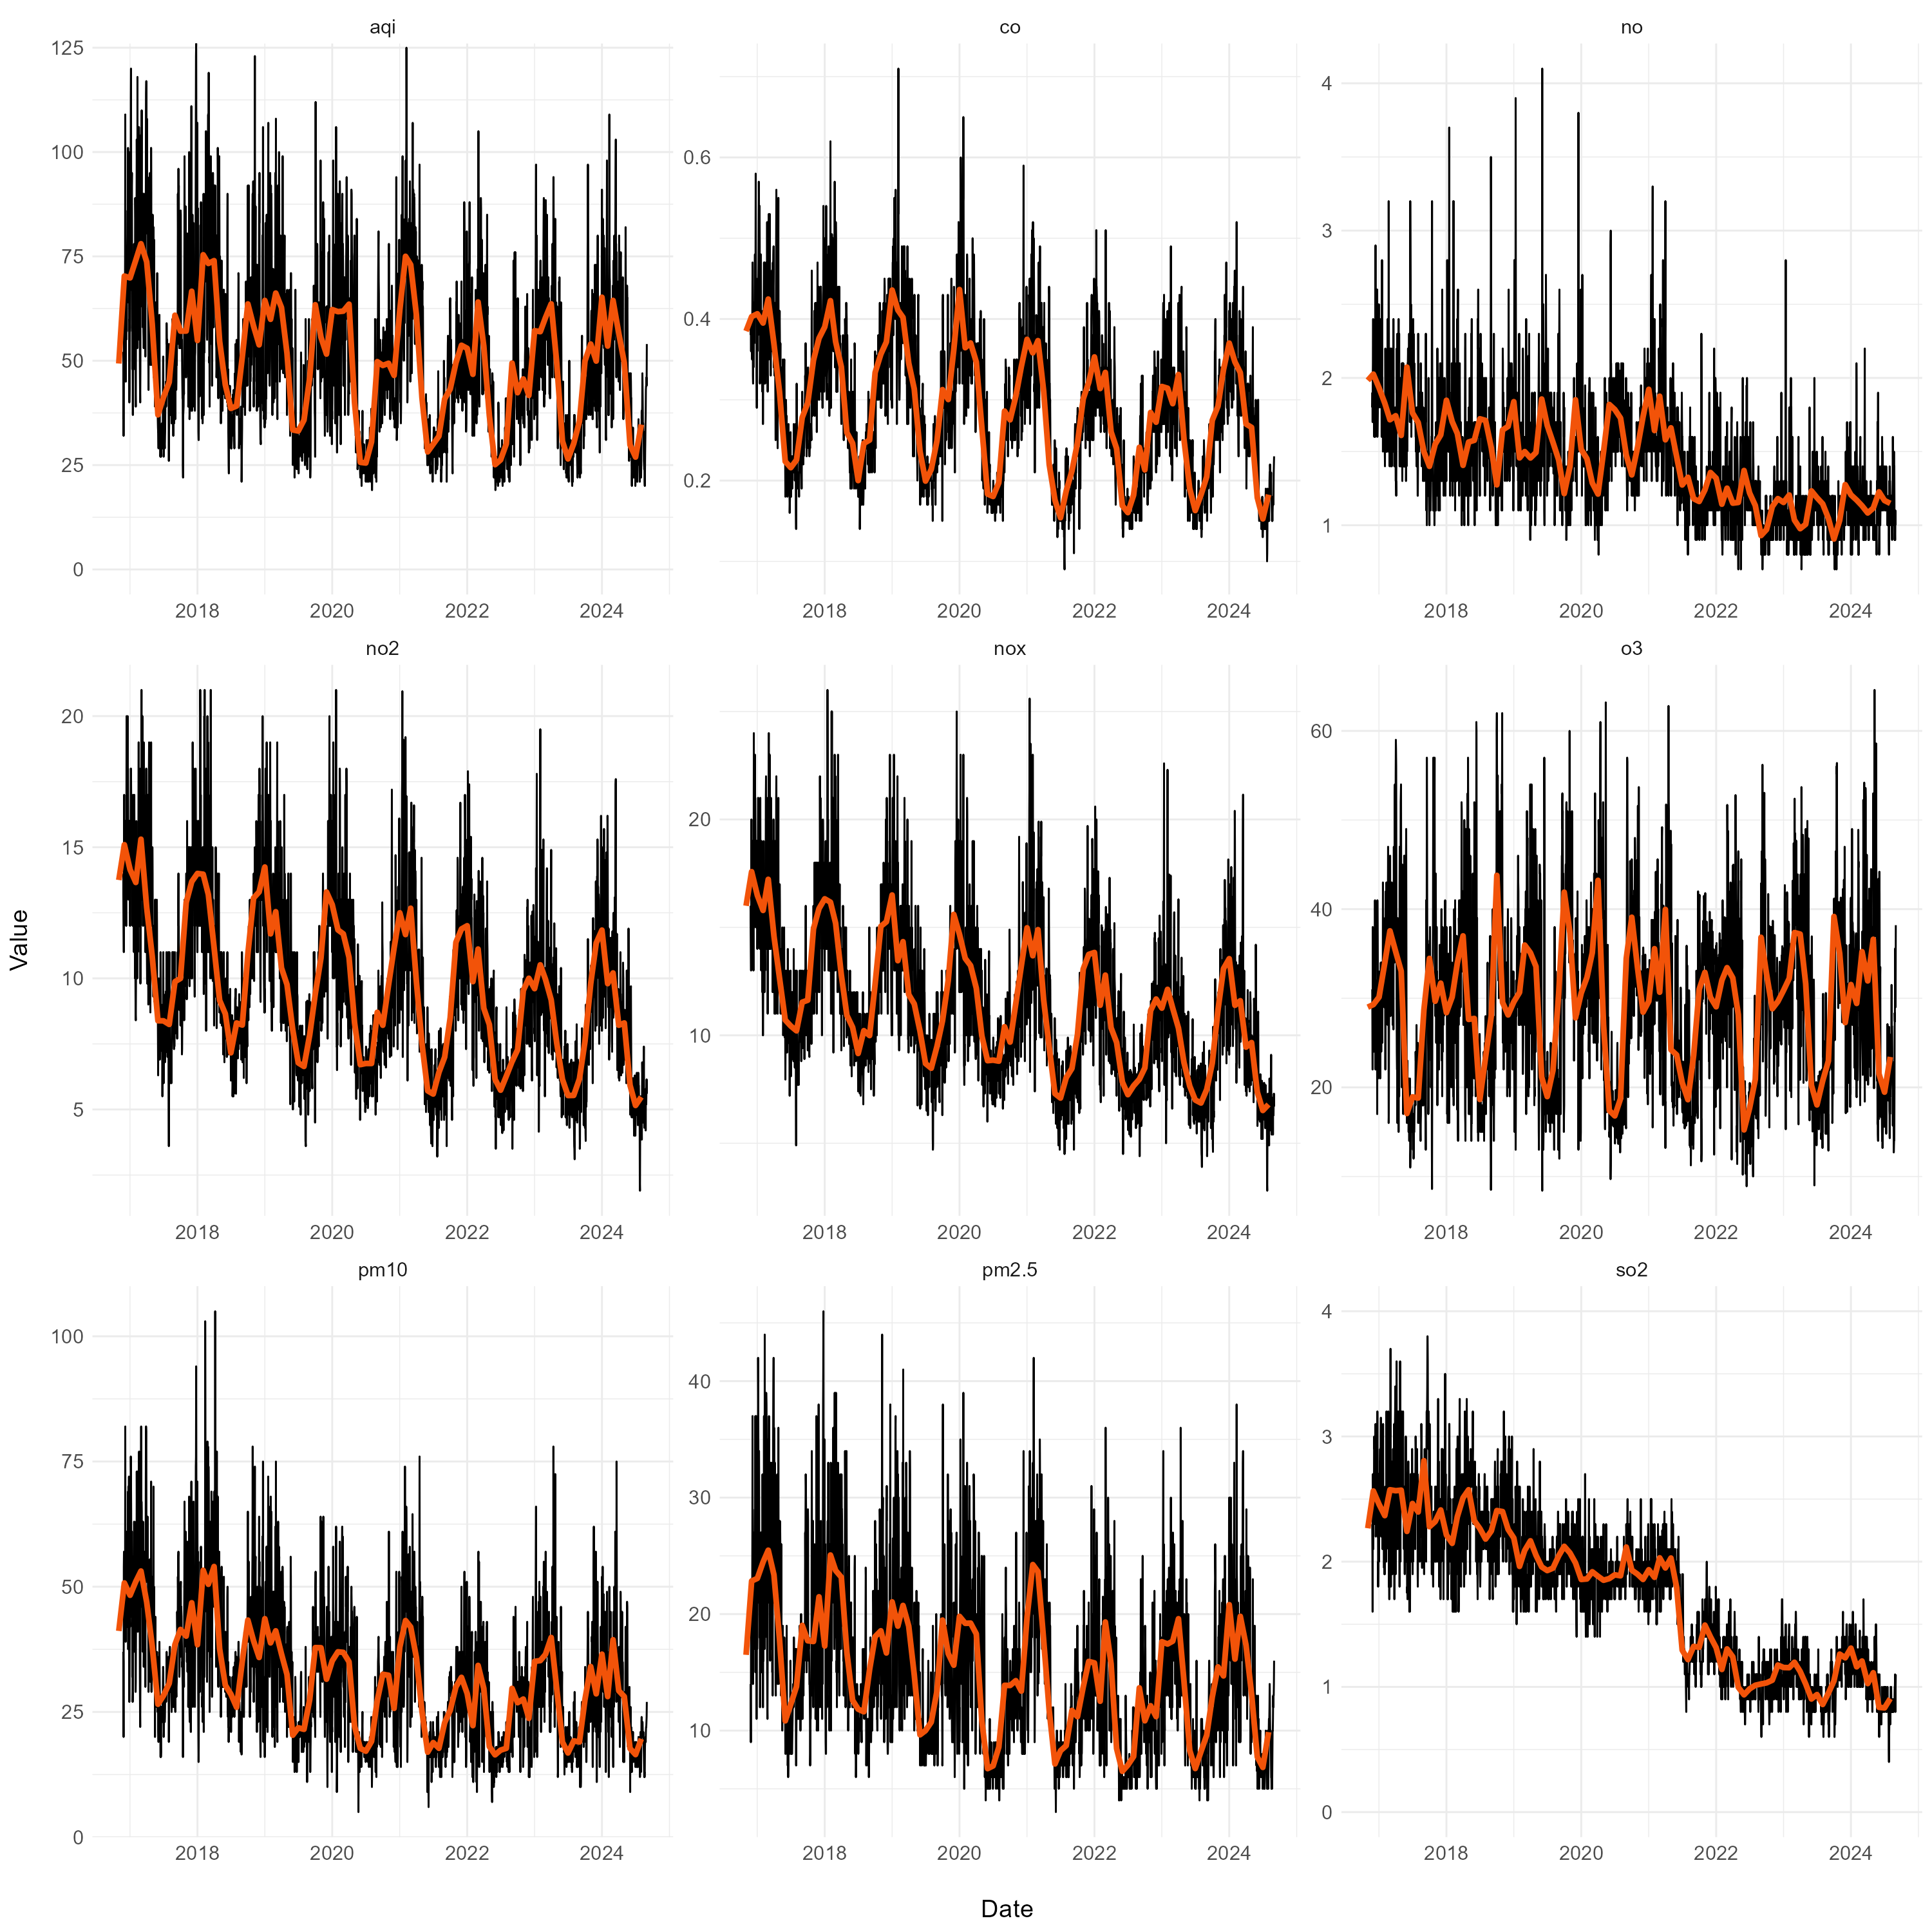
\includegraphics[width=6in]{plots/question6/line.png}

  \item Як змінюється якість повітря залежно від станції виміру у містах?
    
  \quad \textit{Був використаний trimmed набір даних}

  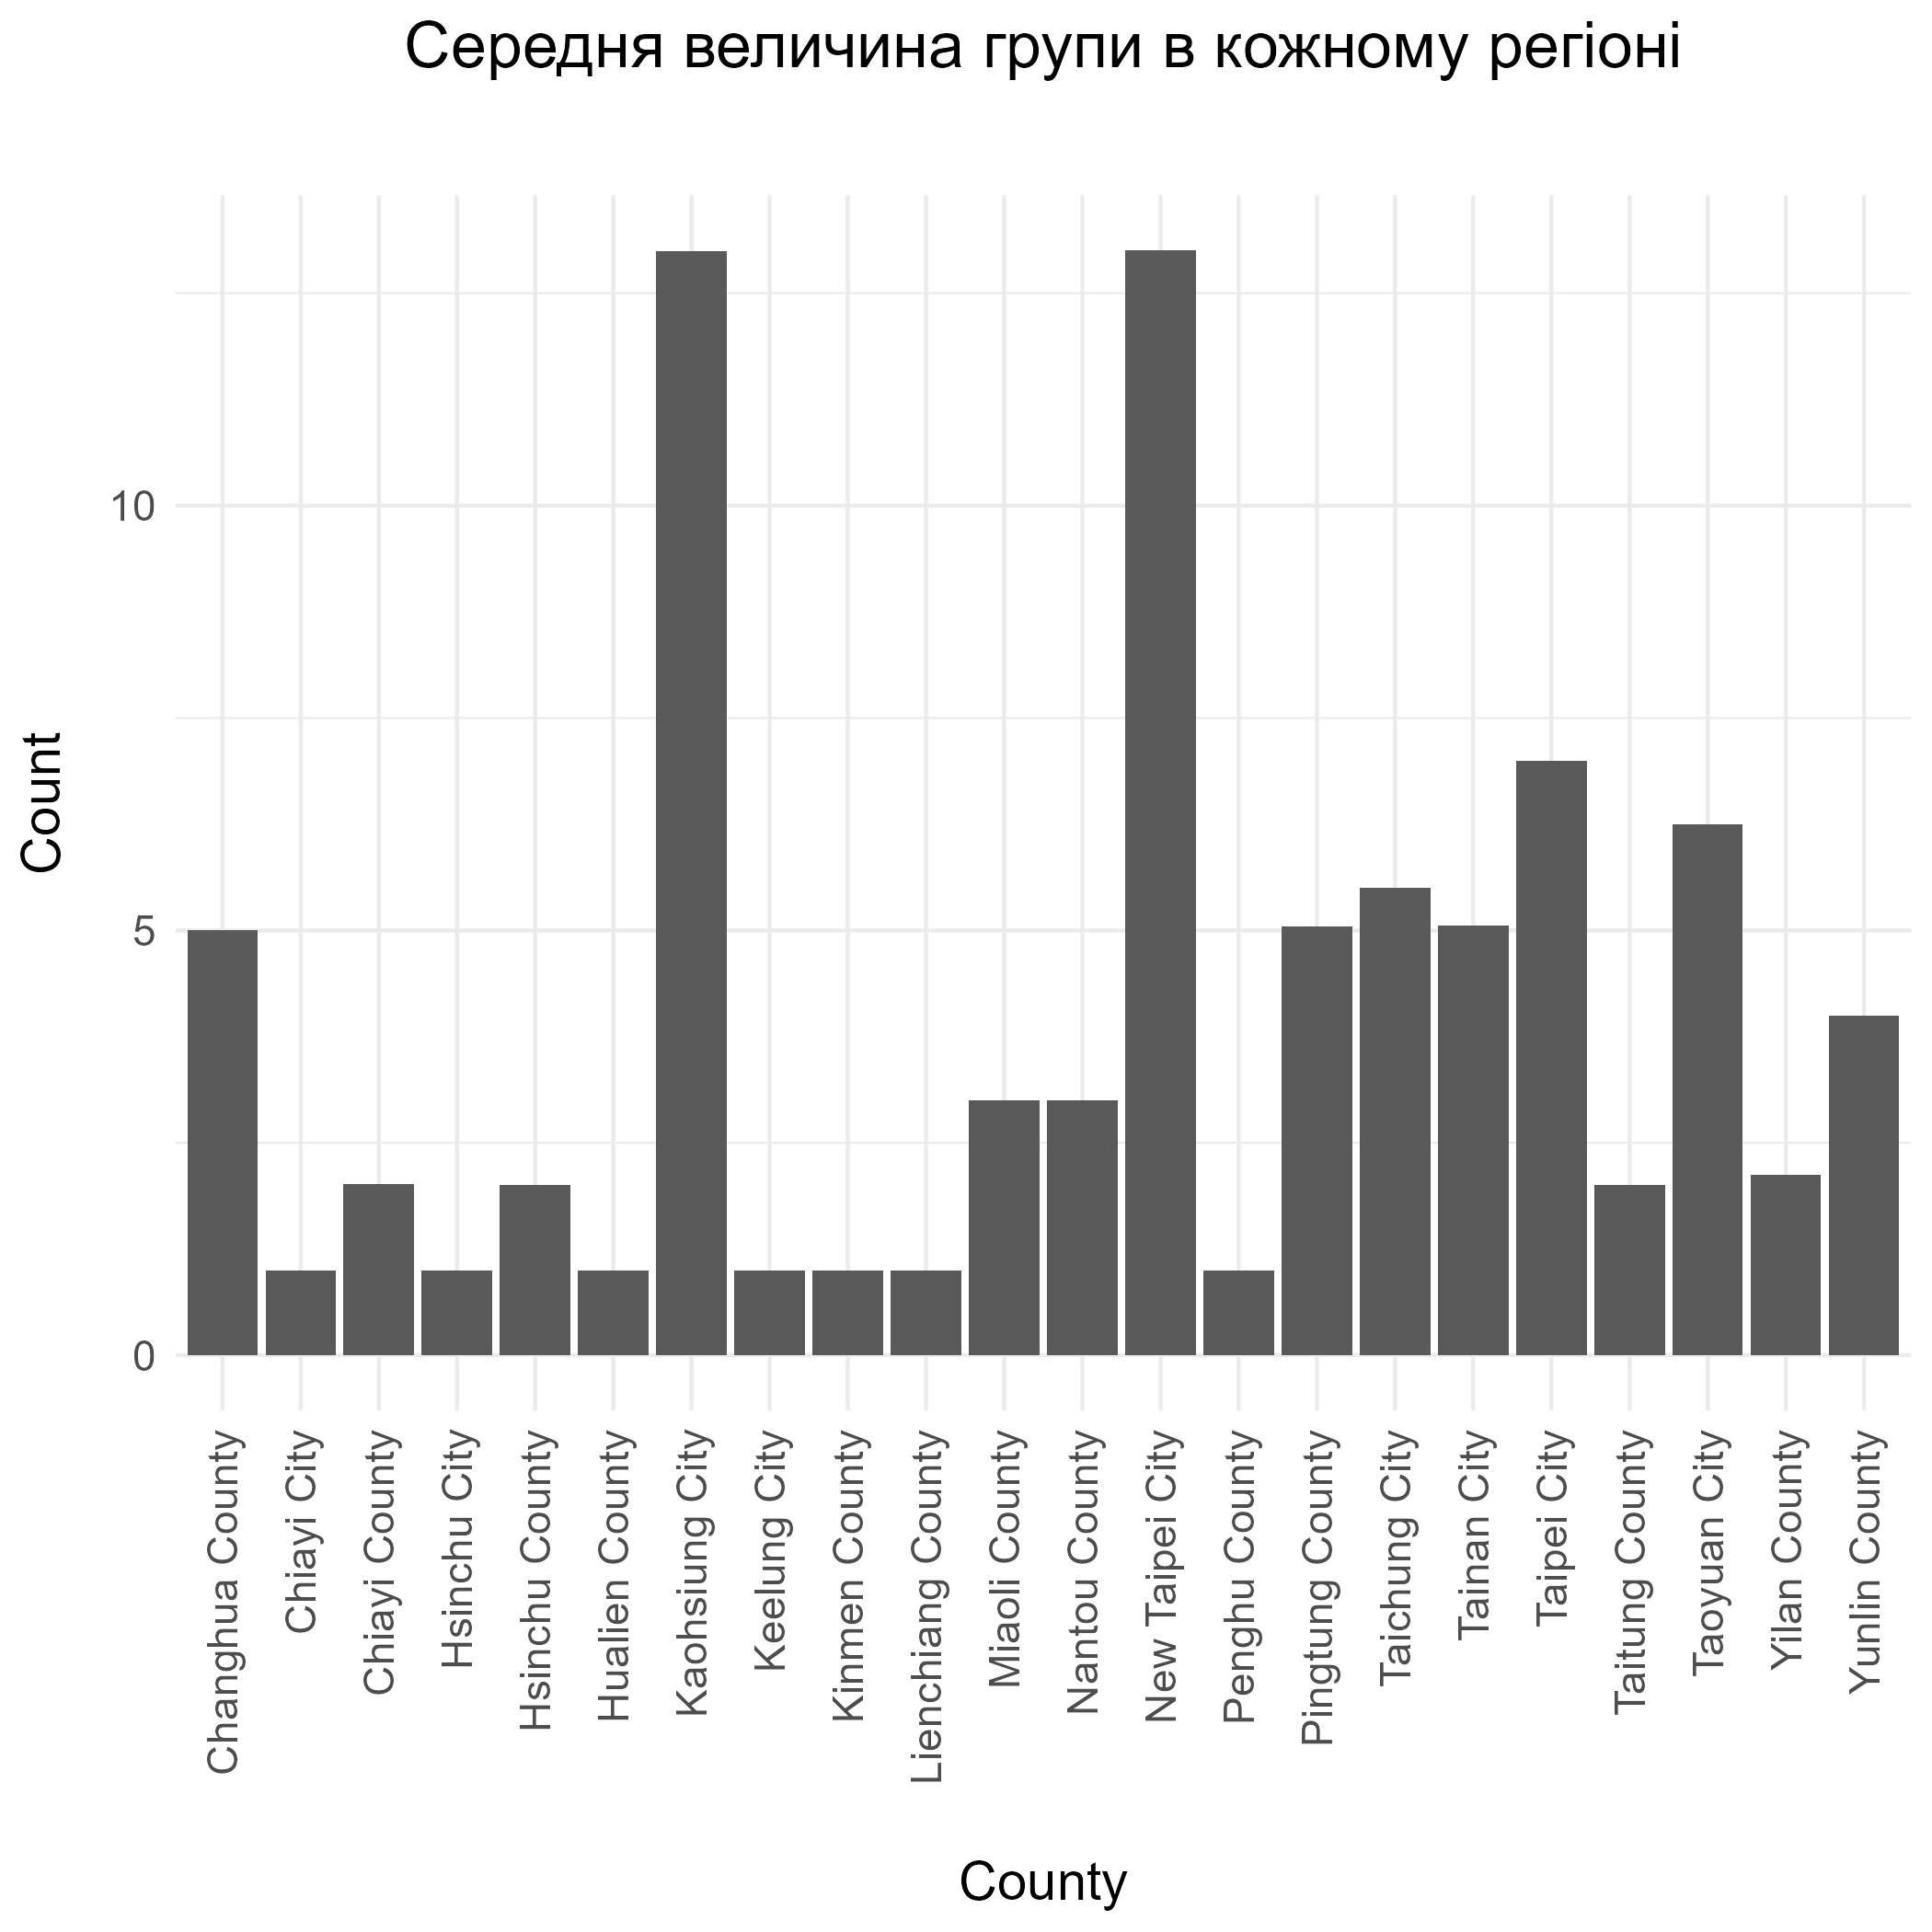
\includegraphics[width=6in]{plots/question7/bar-count.png}
  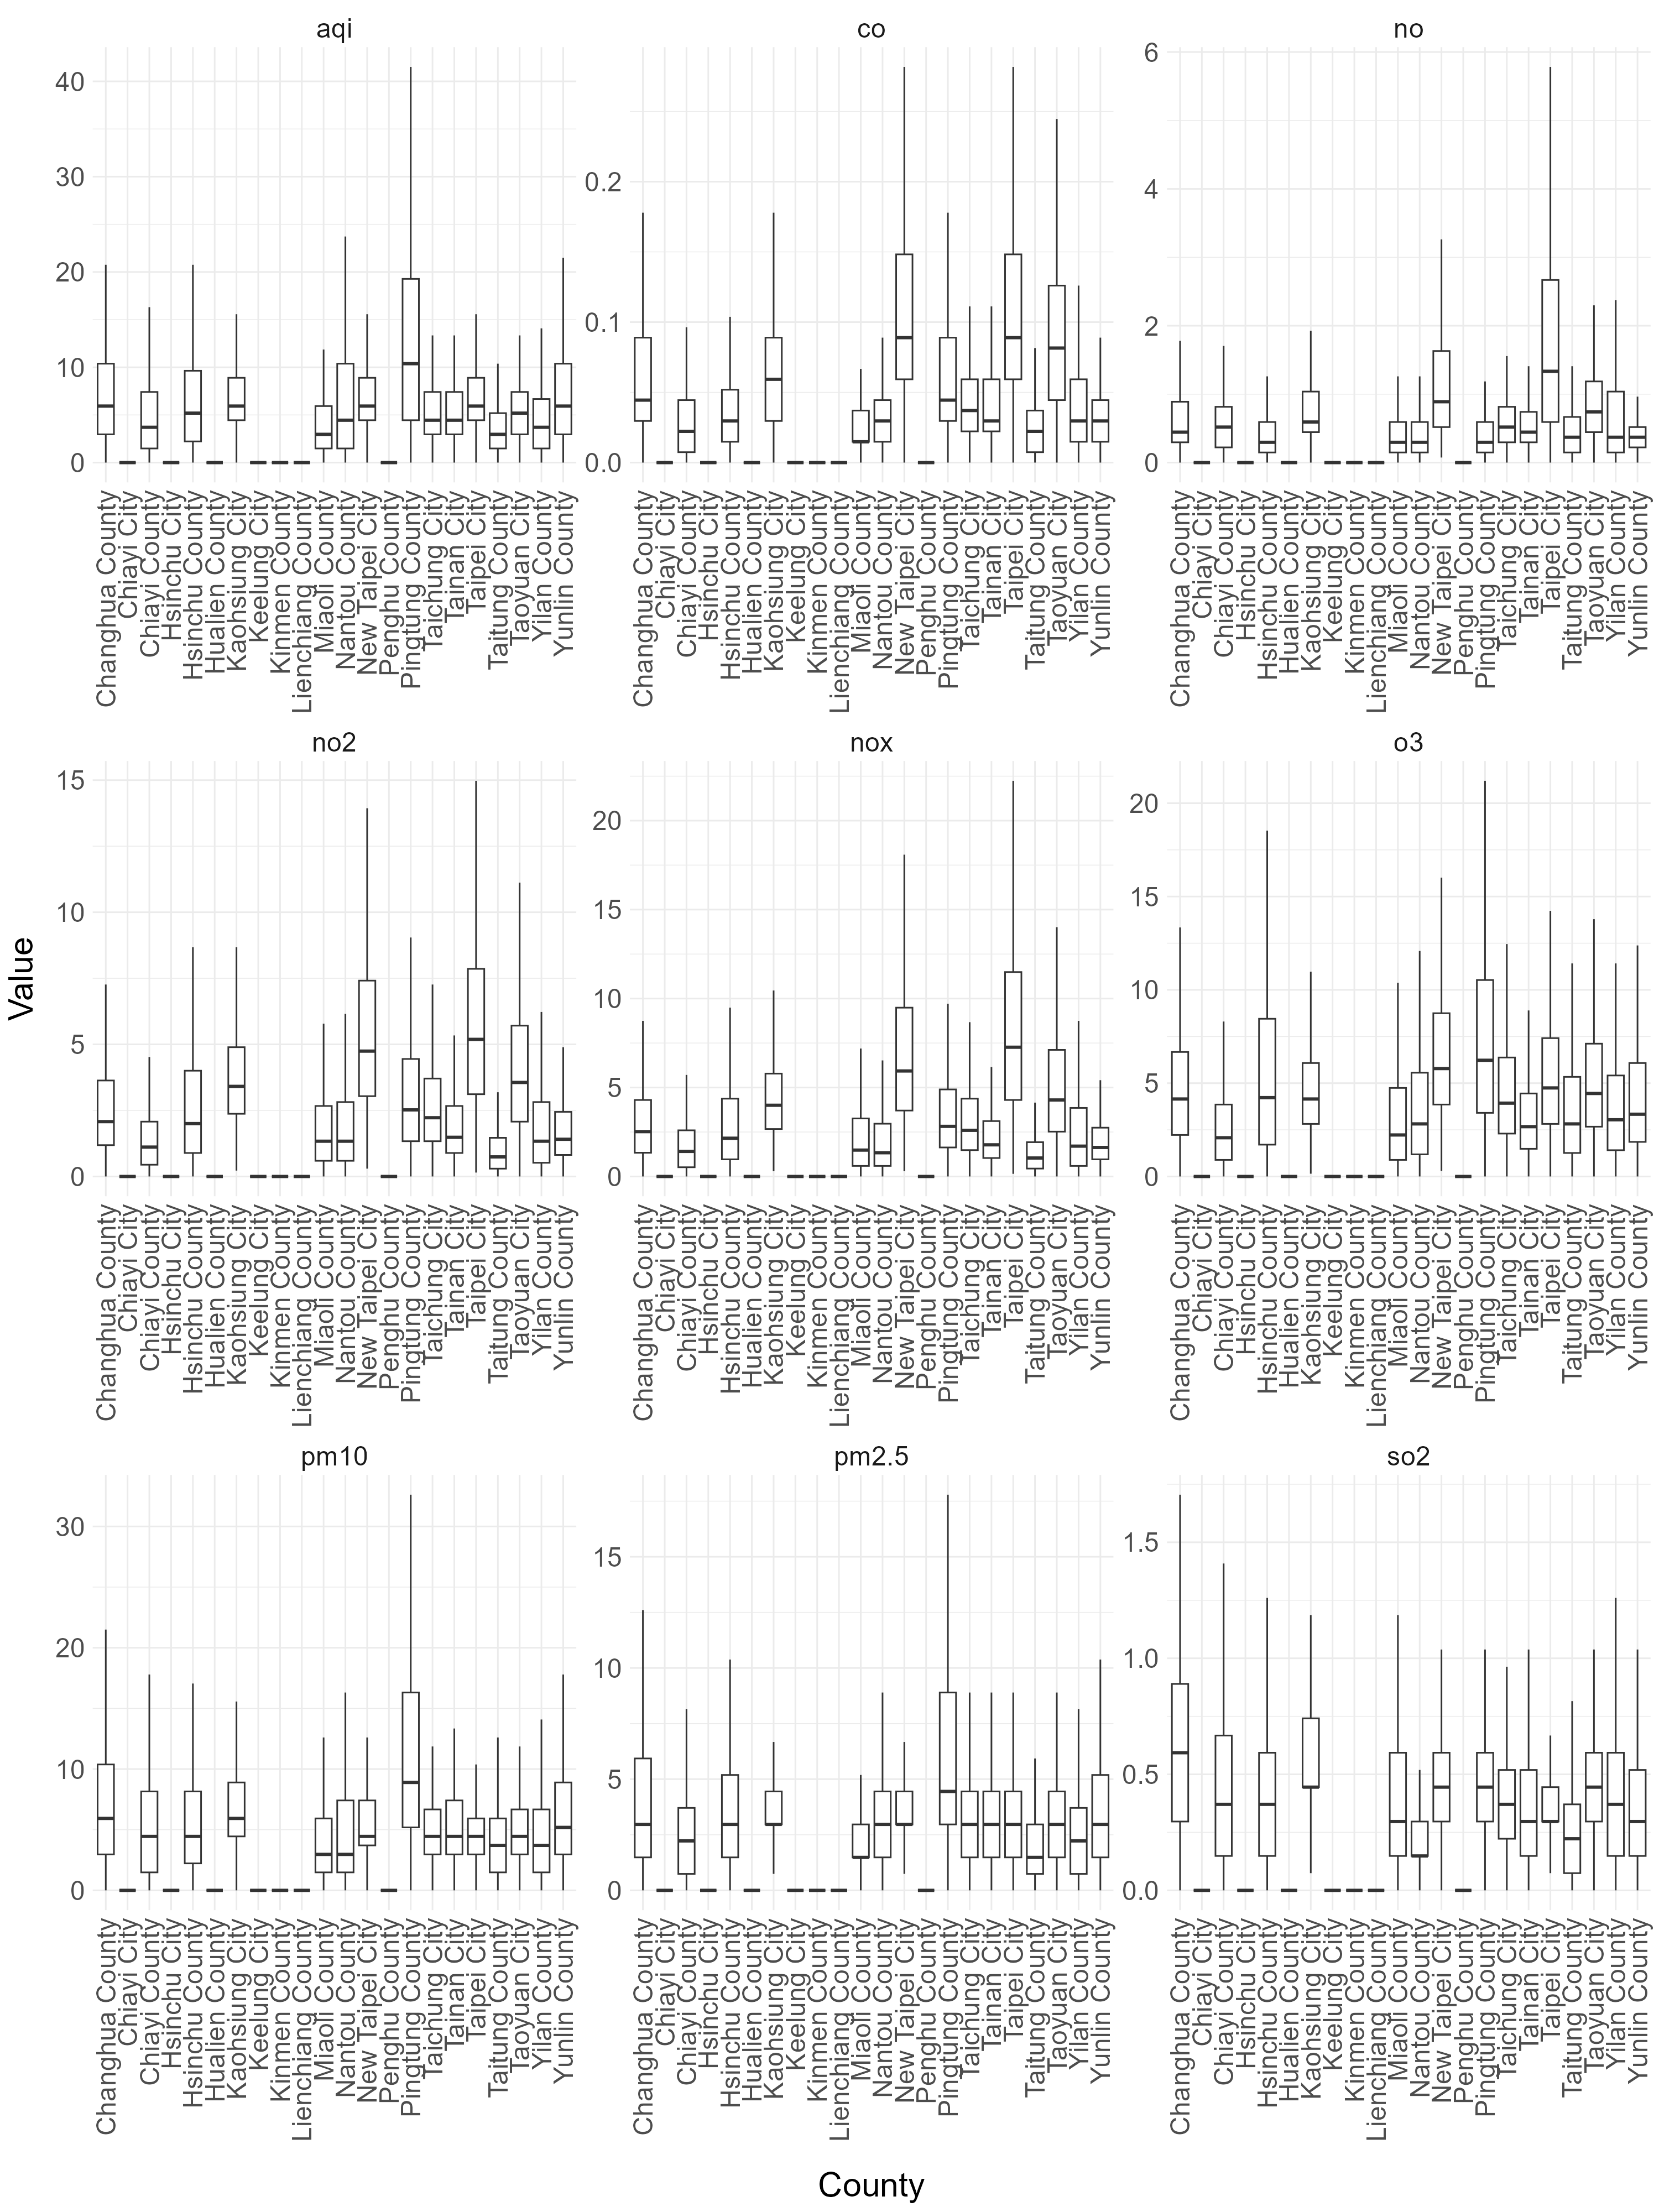
\includegraphics[width=6in]{plots/question7/box-county.png}
  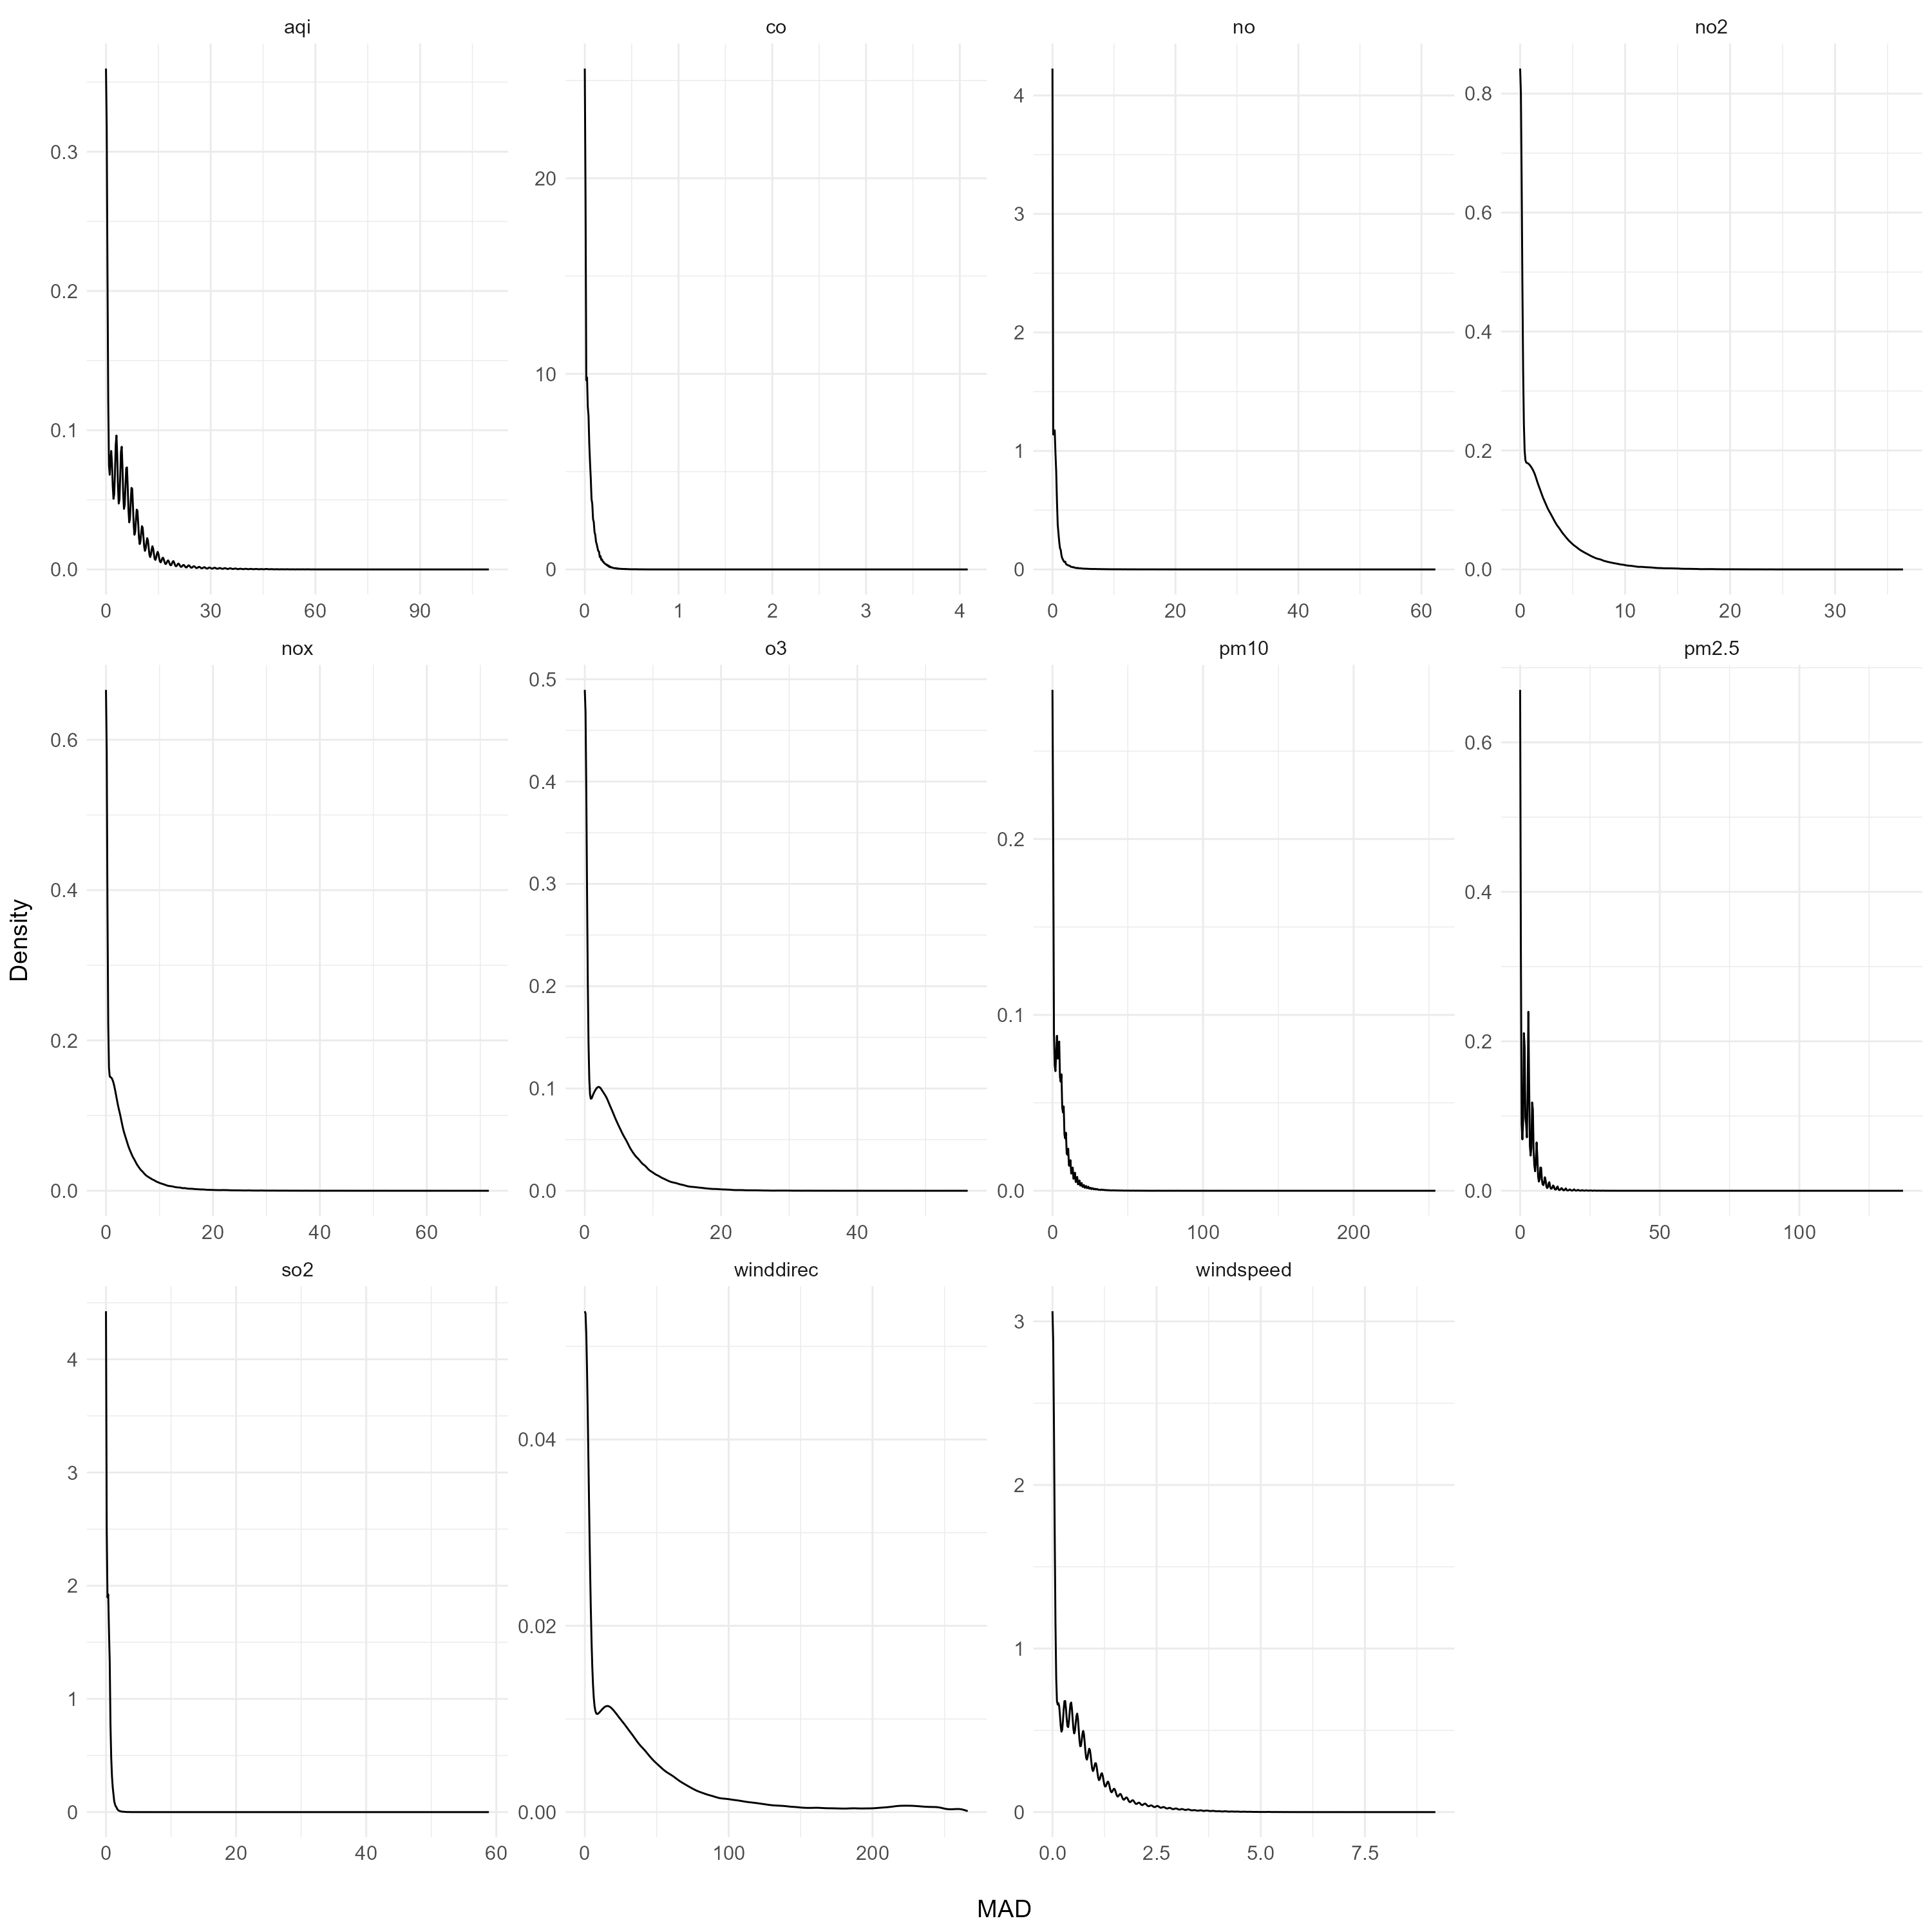
\includegraphics[width=6in]{plots/question7/density.png}
  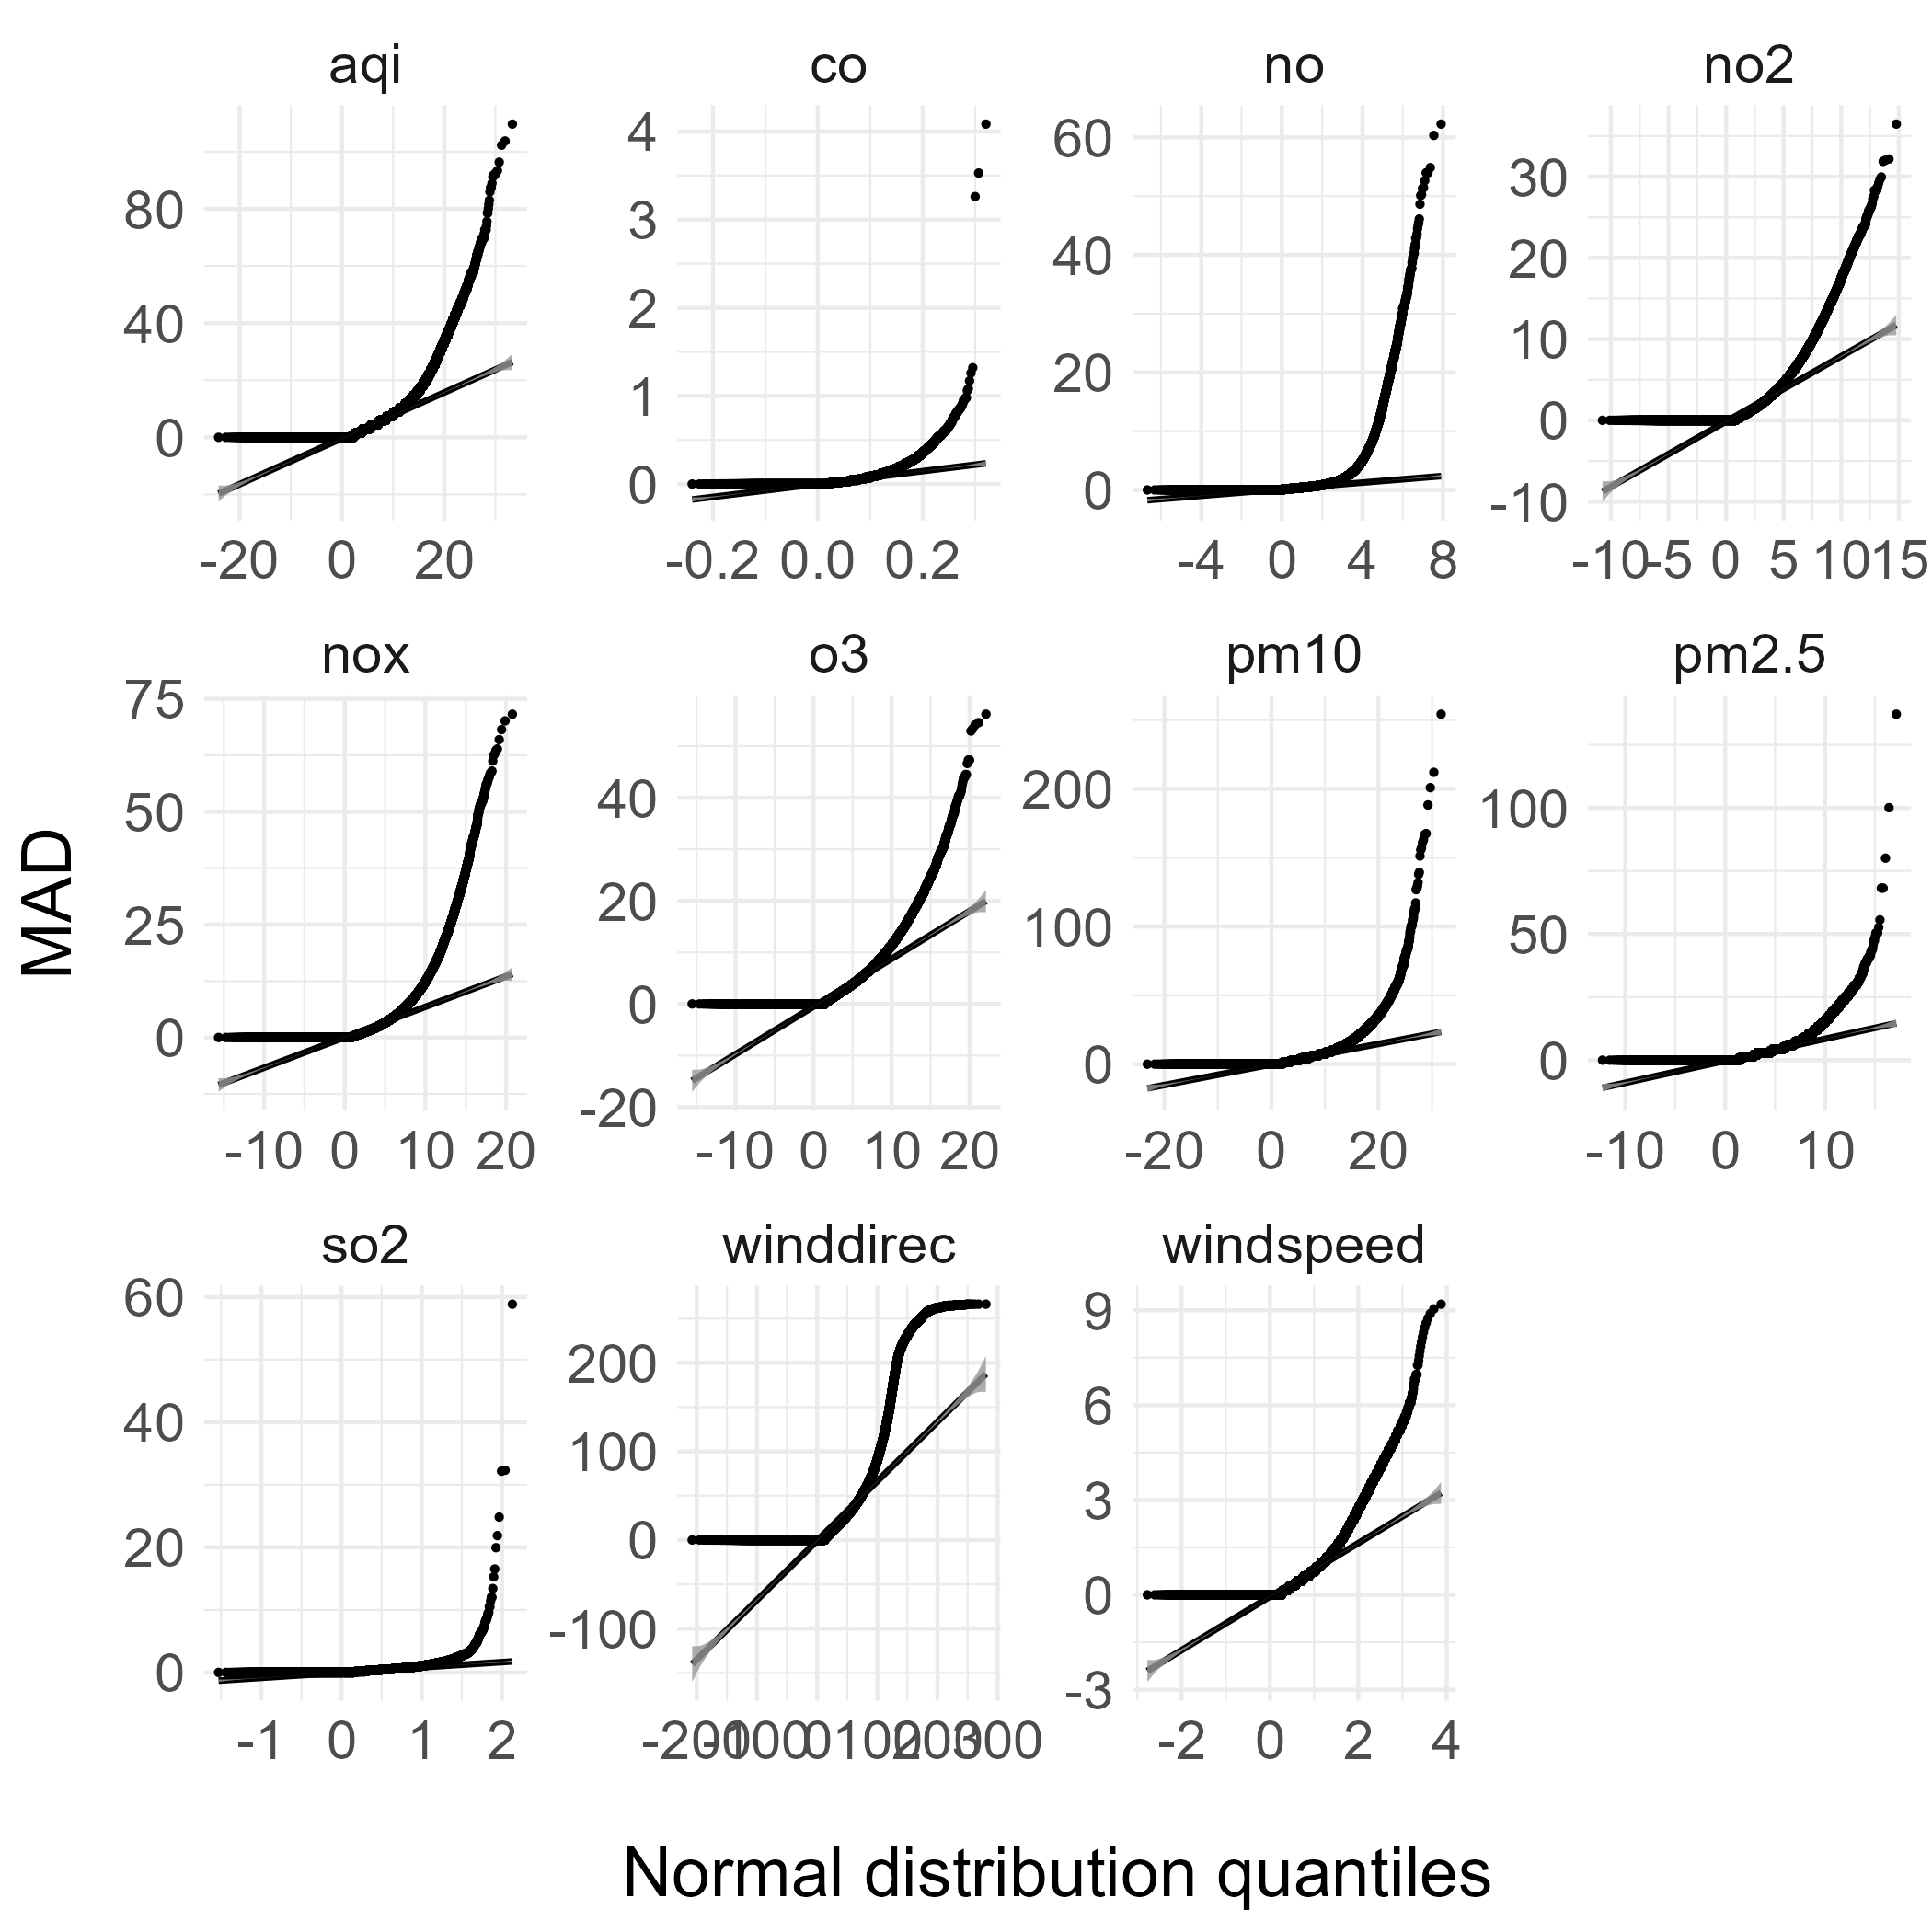
\includegraphics[width=6in]{plots/question7/qq.png}
\end{enumerate}

\end{document}